\chapter{State of The Art} \label{chap:stateOfTheArt}
%\begin{flushright}{\slshape    
%   Science, my boy, is made up of mistakes, but they are mistakes
%   which it is useful to make, because they lead little by little
%   to the truth}. \\ \medskip --- \citeauthor{verne_journey:1957}
%   \citetitle{verne_journey:1957} \citeyear{verne_journey:1957}
%\end{flushright} 

\section{Big Data}\label{sec:big_data}
\lettrine[lines=4]{\textcolor{purple}{T}}{he} term "big data" The term "big data" refers to a  research branch that deals with methodologies to analyze and extract information from data sets containing data that can be structured, like in the traditional relational databases, semi-structured, like in the self-described XML or JSON documents, or unstructured, like in the logfiles collected mostly by web applications to monitor usage or other user's preferences. More properly, we call big data those that cannot be handled using traditional database and software technologies. 
%Today, every second 8,411 Tweets are sent, 902 Instagram photos are uploaded, 1,502 Tumblr posts are created, 3,690 Skype calls are done, 73,116 Google searches are performed and 2,780,000 emails are sent\footnote{Data source: \url{http://www.internetlivestats.com/}}~\cite{misc:InternetLiveStats}. 
IDC~\cite{misc:IDC} has predicted that by 2020 one tenth of the world’s data will be produced by machines. The organisation forecast that in five years time the amount of connected devices communicating over the internet will reach 32 billion and generate 10\% of the world’s data.
This data is collected and analyzed. 
%Gartner's definition of big data is: "Big data is high-volume, high-velocity and/or high-variety information assets that demand cost-effective, innovative forms of information processing that enable enhanced insight, decision making, and process automation"\footnote{\url{https://www.gartner.com/it-glossary/big-data/}}. This defintion relates to something known as the three V's characterizing big data: Volume, Velocity,Variety~\cite{WhatIsBigData}. Volume is important because the amount of data matters. With big data, you’ll have to process high volumes of low-density, unstructured data. This can be data of unknown value, such as Twitter data feeds, clickstreams on a webpage or a mobile app, or sensor-enabled equipment. For some organizations, this might be tens of terabytes of data. For others, it may be hundreds of petabytes. Velocity is the fast rate at which data is received and (perhaps) acted on. Normally, the highest velocity of data streams directly into memory versus being written to disk. Some internet-enabled smart products operate in real time or near real time and will require real-time evaluation and action. Variety refers to the many types of data that are available. Traditional data types were structured and fit neatly in a relational database. With the rise of big data, data comes in new unstructured data types. Unstructured and semistructured data types, such as text, audio, and video require additional preprocessing to derive meaning and support metadata. By means of hardware virtualization, cloud computing services satisfies all the requested requisites needed to manipulate big data. Elasticity and redundancy provided by cloud computing also enable big data application high availability, scalability and fault tolerance.
%Big data also is an unprecedented business opportunity for many companies which  deliver big data applications as a service. According to  SoftwareTestingHelp~\cite{misc:BigDataCompanies}, these are the top 10 big data companies of 2019: IBM~\cite{misc:IBM}, HP Enterprise~\cite{misc:HPE}, Teradata~\cite{misc:Teradata}, Oracle~\cite{misc:Oracle}, SAP~\cite{misc:SAP}, Dell EMC~\cite{misc:EMC}, Amazon~\cite{misc:AWS}, Microsoft~\cite{misc:Microsoft}, Google~\cite{misc:Google}, VMware~\cite{misc:VMware}.

\subsection{Batch Processing: Hadoop}\label{sec:map_reduce_hadoop}
%\section{Hadoop}\label{sec:hadoop}
MapReduce is a software framework introduced by Google in order to support the distributed computation of large dataset in cluster of computers. The framework is inspired by map and reduce functions used in functional programming, even though their purpose in the MapReduce framework is not the same as in the original form.
There are available MapReduce libraries written in different programming languages. 
\begin{figure}
	\centering
	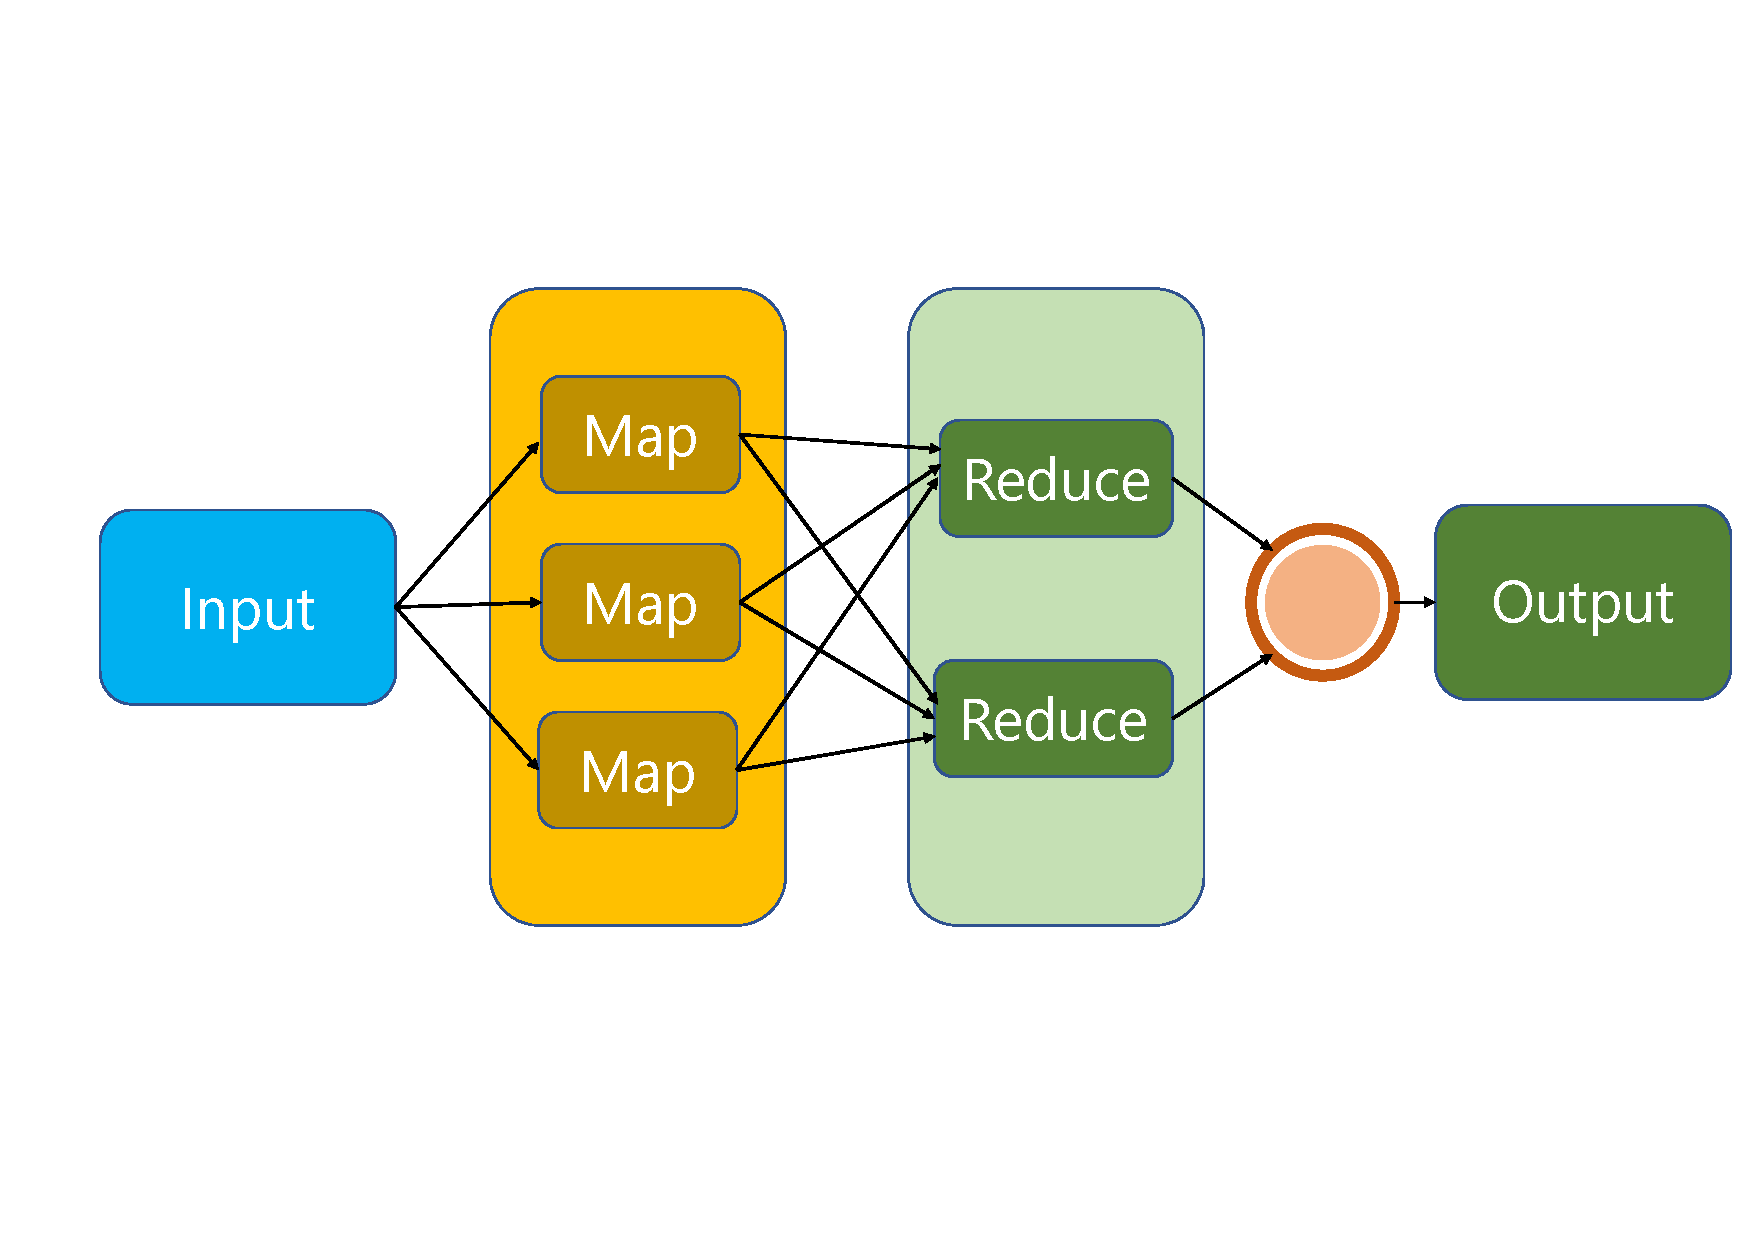
\includegraphics[width=\columnwidth]{Images/map_reduce_1.pdf}  
	\caption[map-reduce model]{Abstract representation of map-reduce paradigm}
	\label{fig:mapReduce}
\end{figure}

MapReduce is a programming framework that allows us to perform distributed and parallel processing on large data sets in a distributed environment.\footnote{Extracted from: https://www.edureka.co/blog/mapreduce-tutorial/}.
\begin{itemize}
	\item MapReduce consists of two distinct tasks – Map and Reduce.
	\item As the name MapReduce suggests, reducer phase takes place after mapper phase has been completed.
	\item So, the first is the map job, where a block of data is read and processed to produce key-value pairs as intermediate outputs.
	\item The output of a Mapper or map job (key-value pairs) is input to the Reducer.
	\item The reducer receives the key-value pair from multiple map jobs.
	\item Then, the reducer aggregates those intermediate data tuples (intermediate key-value pair) into a smaller set of tuples or key-value pairs which is the final output.
\end{itemize}

There are open source implementation of the MapReduce framework, for example Apache Hadoop.
The MapReduce framework is composed by different functions for each step:
\begin{enumerate}
	\item Input Reader
	\item Map Function
	\item Partition Function
	\item Compare Function
	\item Reduce Function
	\item Output Writer
\end{enumerate}

The Input Reader reads the data from mass memory and splits the input in S different splits, with a fixed dimensions (e.g., 64 MB) that are successively distributed to M machines of the cluster that have the Map Function. The Input Reader has also the goal of generating a pair (key, value). The N machine of the cluster are divided in 1 master,
whose goal is to detect idling slaves and assign them a task, and N - 1 slaves that receive the tasks assigned by the master node. In total, M Map tasks and R Reduce tasks are assigned. A slave that has been assigned the M-th task reads the content of the input, extracts the (key, value) pairs and send them to the Map function defined
by the user, that generates zero or more (key, value) pairs as output. These pairs are buffered in memory. Periodically the buffered pairs are cached on disk and partitioned in R sections by the partition function. The addresses of the partitioned sections are sent to the master node which is responsible of rotating the location of the slaves that
will process the Reduce function. Between the slave with the Map function and the one with the Reduce one, all the pairs are reordered in order to find the ones that point at the same value, and thus also have the same key.  
The so called shuffling phase is the process that is used to transfer data from mappers to reducers. Once all the keys that point to the same value have been found using the compare function, a merge operation is performed. The sorting operation is useful because in this way the reducer can know when a new reduce task should start. For each of the keys, the associated slave iterates on all the keys, takes the values with the same key and then applies the Reduce function defined by the user, generating one or more element in output. The Output Writer has the goal of writing the results back to mass storage.
\begin{figure}
	\centering
	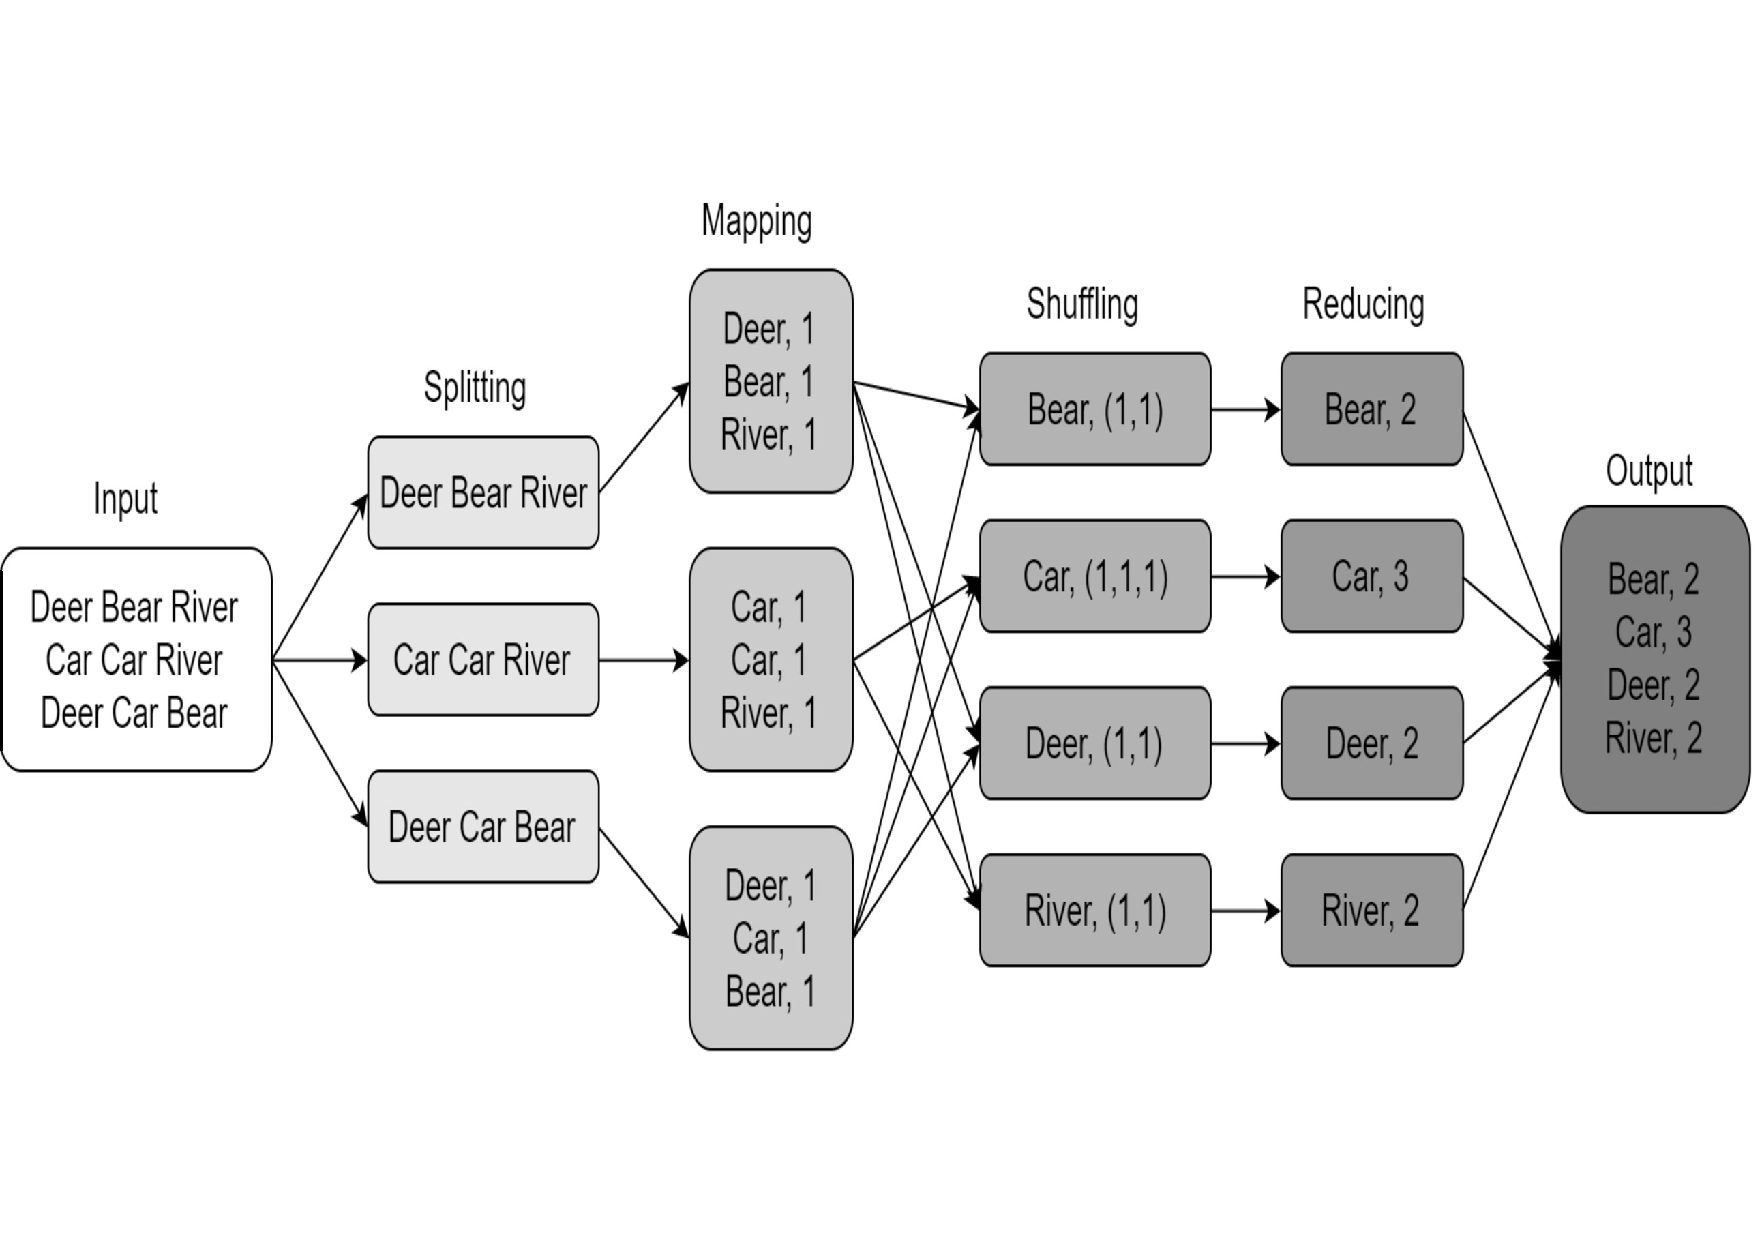
\includegraphics[width=\columnwidth]{Images/word_count_example.pdf}  
	\caption[map-reduce model]{Map-Reduce word count job example. Counts the occurrence of each word in input}
	\label{fig:wordCountExample}
\end{figure}
A sample word count application can be seen in \myFig{fig:wordCountExample} The input is a document containing words, our goal is to compute the number of occurrence of each of the words in the document. Each Map task applies its function on a line of the document, emitting for each of the words in the line a pair (’word’, 1). For example if the input line is "Dear Bear River", it is split into ["Dear", "Bear", "River"] and then mapped into [("Dear", 1), ("Bear", 1), ("River", 1)]. After shuffling the map results, the Reduce task receives a word and a list containing as many ones as the times the word appeared in the document, the reduce function will simply sum the ones in the list, emitting as a
result the pair (’word’, ’count’). For example, a reducer can receive the key "Bear" with list of values (1, 1), this is reduced into ("Bear", 2). Reducers results are then collected and stored in mass storage.

Apache Hadoop\footnote{url: https://hadoop.apache.org/docs/} is an open-source framework for distributed storage and processing of big datasets using MapReduce programming model.

\begin{figure}
	\centering
	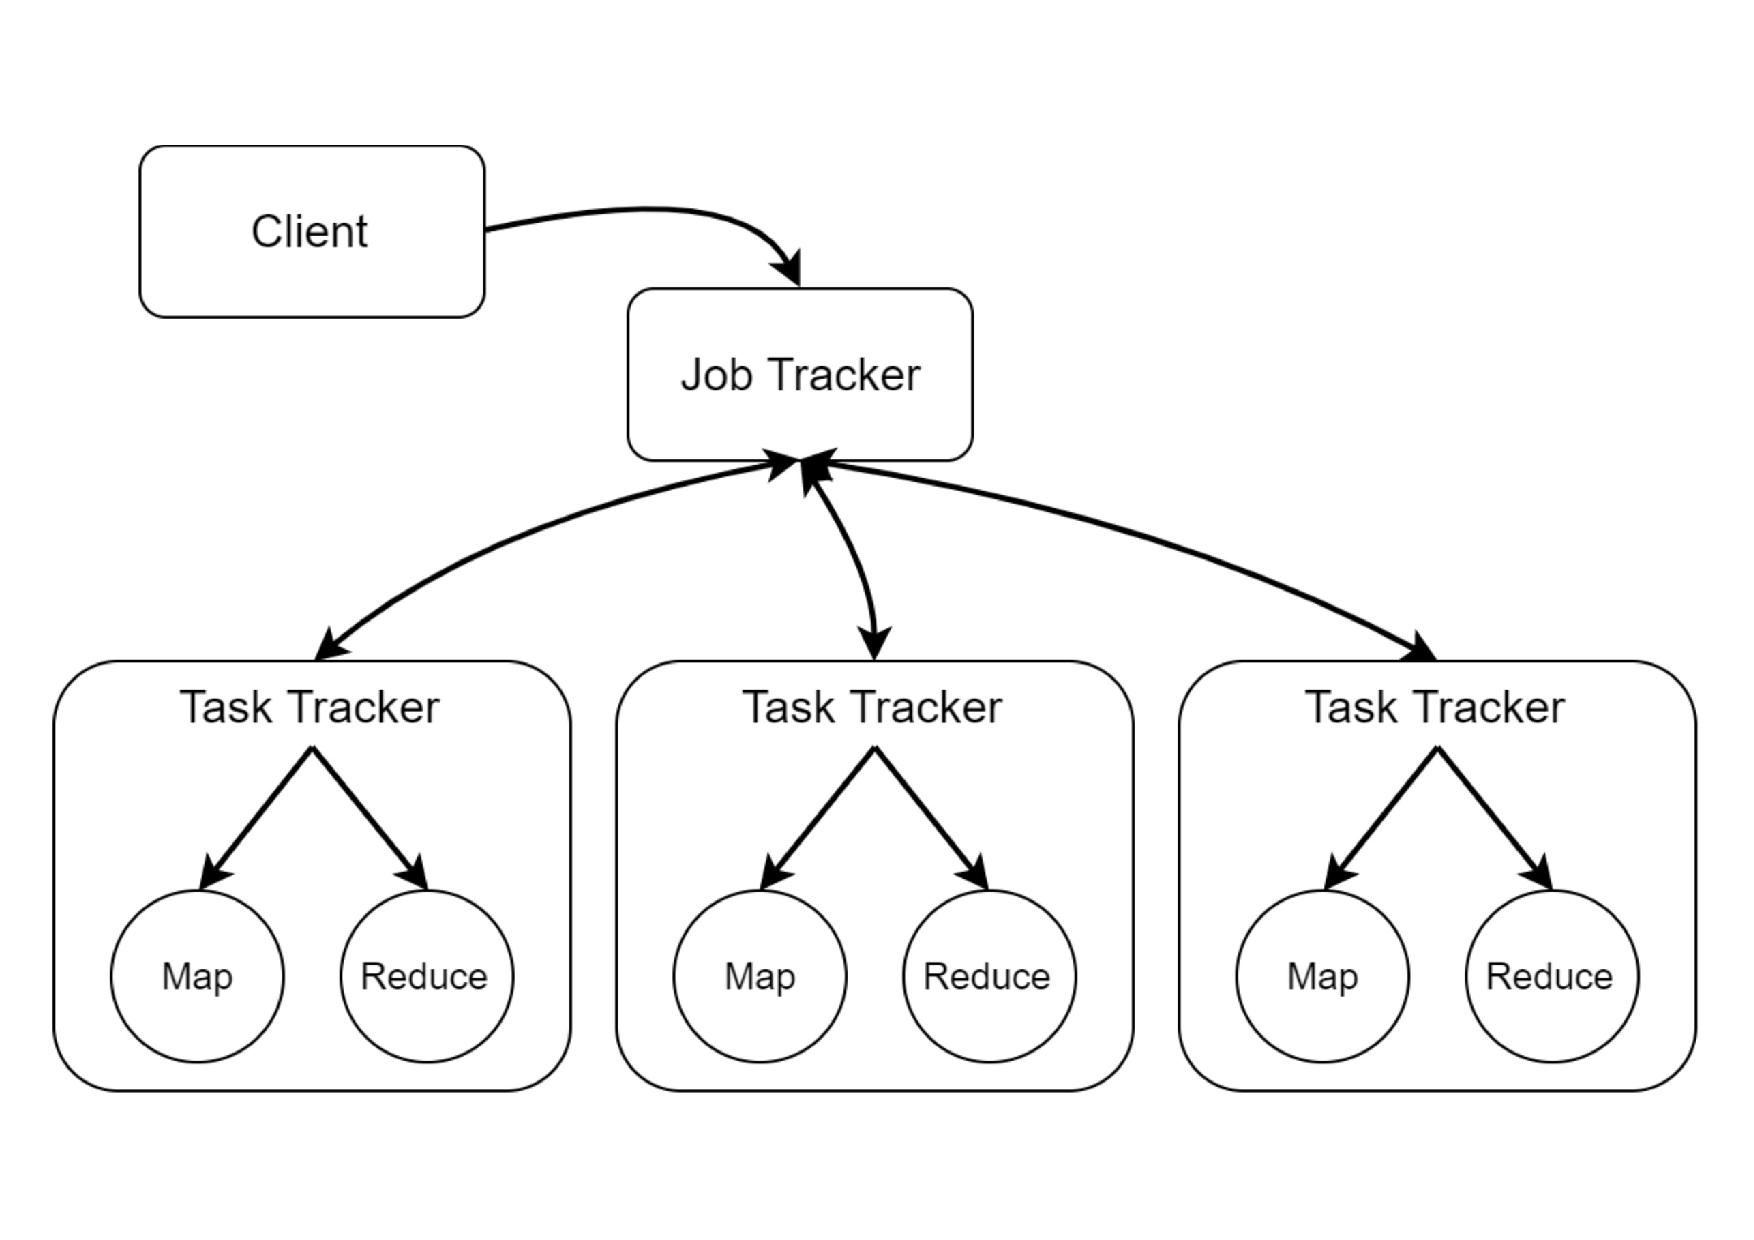
\includegraphics[width=\columnwidth]{Images/hadoop_map_reduce_architecture.pdf}  
	\caption[hadoop map-reduce architecture]{Hadoop Map-Reduce Architecture.}
	\label{fig:hadoopMapReduceArchitecture}
\end{figure}

Apache Hadoop MapReduce cluster have a centralized structure
composed by a single master Job Tracker (JT) and multiple worker nodes running Task Tracker (TT), as shown in  \myFig{fig:hadoopMapReduceArchitecture} JT main goal
is organizing the job tasks on the slave nodes and continuously monitor
the Task Trackers by means of heartbeats. Heartbeats provide a way to retrieve information about the liveliness of the slaves and to
inspect the progress of the executions of the different tasks. In order
to be fault tolerant, if a task execution fails, it is re-executed possibly
on a different slave. JT has the role of the cluster manager, so it
needs also to check the admissibility of the submitted MapReduce
jobs. TT have the objective of running the assigned task. They reply to
heartbeats in order to affirm their liveliness and to update the master
about the progress of the assigned tasks. They are configured with a
fixed number of map and reduce task slots.
As previously introduced, Apache Hadoop also offers a distributed file-system that stores data on different machine, 
providing an high aggregate bandwidth across the cluster. This functionality is called Hadoop Distributed File System (HDFS)\footnote{\textit{HDFS Architecture Guide.} url:  https://hadoop.apache.org/docs/r1.2.1/hdfs\_design.html}. 
It is highly fault tolerant and designed to be deployed on low cost hardware.
\begin{figure}
	\centering
	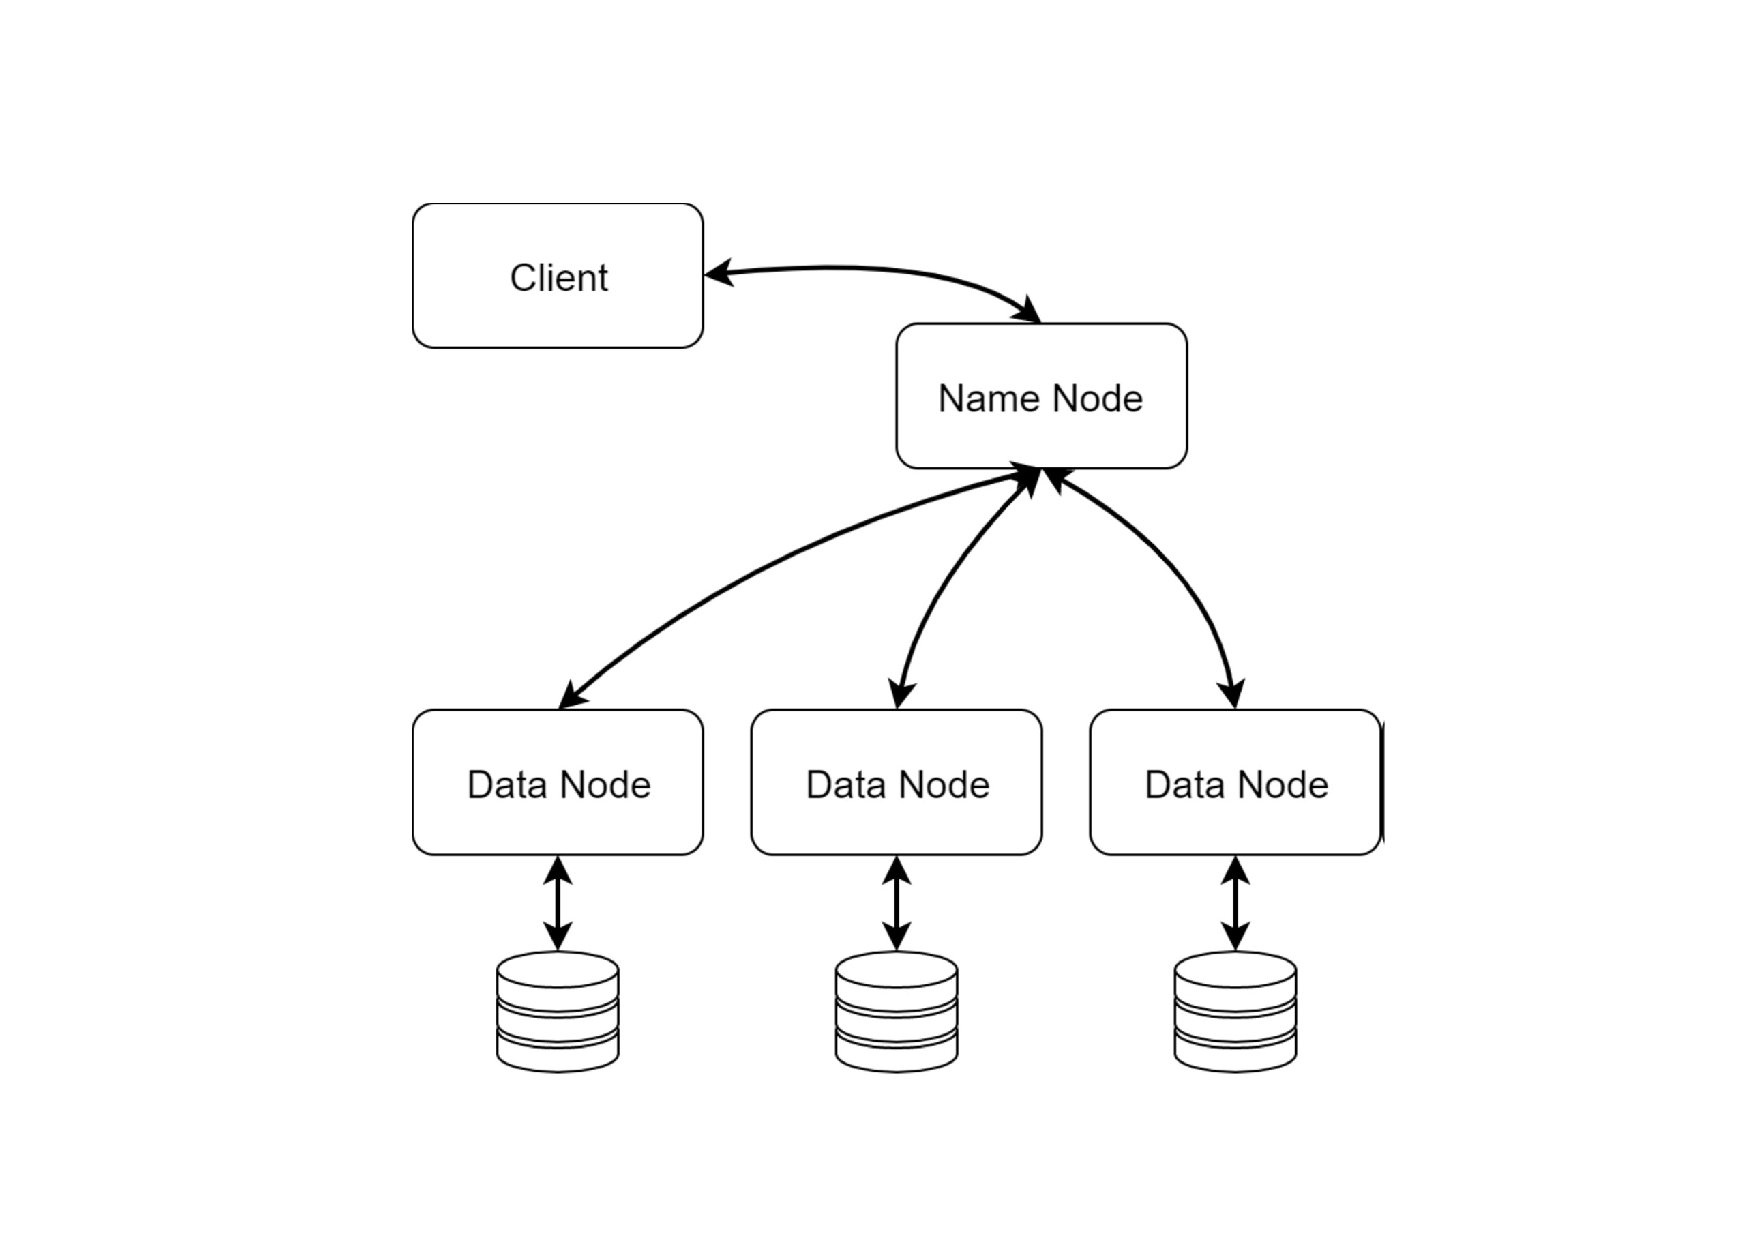
\includegraphics[width=\columnwidth]{Images/hdfs_1.pdf}  
	\caption[HDFS Node Strucure]{HDFS Node Strucure.}
	\label{fig:hdfsNodeStruct}
\end{figure}
HDFS exposes a filesystem namespace and allows user data to be stored in files and
retrieved. Cluster structure is similar to the one of MapReduce cluster,
with one master and multiple slaves, as we can see from \myFig{fig:hdfsNodeStruct}.
The master is composed by a single Name Node (NN), that manages
the file system namespace and regulates access to the files by clients.
NN executes filesystem operations such as opening, closing, renaming
files and directory, but the most important operation performed is
keeping track of the mapping between blocks and Data Node (DN).
Indeed a file stored in HDFS is split into one or more blocks, and those
blocks are stored in the Data Node (DN). Data Node (DN) represent
the slaves, they are usually one per node, and manage the storage that
is attached to the node they are running on. They are responsible for
serving read and write operation requests from the clients, but also
can perform block creation, deletion and replication. Block replication
is a significant way to improve fault tolerance.

\subsection{Batch Processing: Spark}\label{sec:spark}
Apache Spark is an open source framework for distributed computation
~\cite{misc:ApacheSpark}, that provides an interface for programming entire clusters
with implicit data parallelism and fault tolerance. With respect to the MapReduce paradigm, the in-memory multilevel primitives of Spark allow to have performances up to 100 times better in certain applications. Spark can work as standalone or on a cluster manager such as Apache Hadoop Yarn or Apache Mesos. It also needs a distributed storage and can natively use HDFS and other solutions. 

Spark has been designed as a unified engine for distributed data processing. Its programming model resembles the one of MapReduce, but it is extended with a data sharing abstraction called Resilient Distributed Dataset (RDD). Using this abstraction, a wide range of processing workloads can be captured, including SQL, streaming, machine learning and graph processing. The generality of the Spark approach gives great benefits: firsty, applications are easier to develop since there is a unified API,  secondly, it is a lot easier to combine processing tasks. With previous distributed computation framework we needed to write data to mass storage before using them in another engine. Spark, instead, can reuse the same data, often kept in memory.
The programming abstraction at the foundation of Spark is the Resilient Distributed Dataset (RDD), that is a fault-tolerant collection of objects partitioned across the cluster and can be processed in parallel. The users create RDD's by applying operations called "transformations", such as map, filter and group-by, on the data. RDD's can be
backed by a file obtained from an external storage. Spark evaluates RDD's in a lazy mode. This allows the construction of an efficient plan to execute the computation requested by the user. In particular, every transformation operation returns a new RDD, that is the representation of the result of the computation, but the computation is not executed immediately after the transformation request is encountered, but only when a Spark action is met. When an "action" is requested by the user code, Spark checks the entire graph of the transformation and uses it to create an efficient execution plan. For example, if there are many filters and maps in a row, Spark can merge them together and execute as a single operation.
RDDs also offer an explicit support to data sharing among the computations that are ephemeral by default, but can be persisted to disk or memory for rapid reuse. This data sharing is one of the main differences between Spark and the previous computing models
like MapReduce, because all the other operations that Spark can perform are similar to the ones of MapReduce. The data sharing capability allows huge speedups, up to 100 times, in particular when executing interactive queries and iterative algorithms.
RDDs can also recover automatically from a failure. Traditionally, fault tolerance in distributed computing was achieved by means of data replication and checkpointing. Spark instead uses a different approach called lineage. Each RDD keeps track of its transformation graph used to generate the RDD and re-executes the transformation operations on the base data to recover every lost partition. The data recovery based on lineage is significantly more efficient than replication in case of data-intensive workload. In general, recovering lost partitions is faster than re-executing the entire program. Spark was designed to support different external systems for persistent storage, usually it is used in conjunction with a clustered file system like HDFS. Spark is designed as a storage-system-agnostic engine, to make it easy to run computations against data from different sources.
\begin{figure}
	\centering
	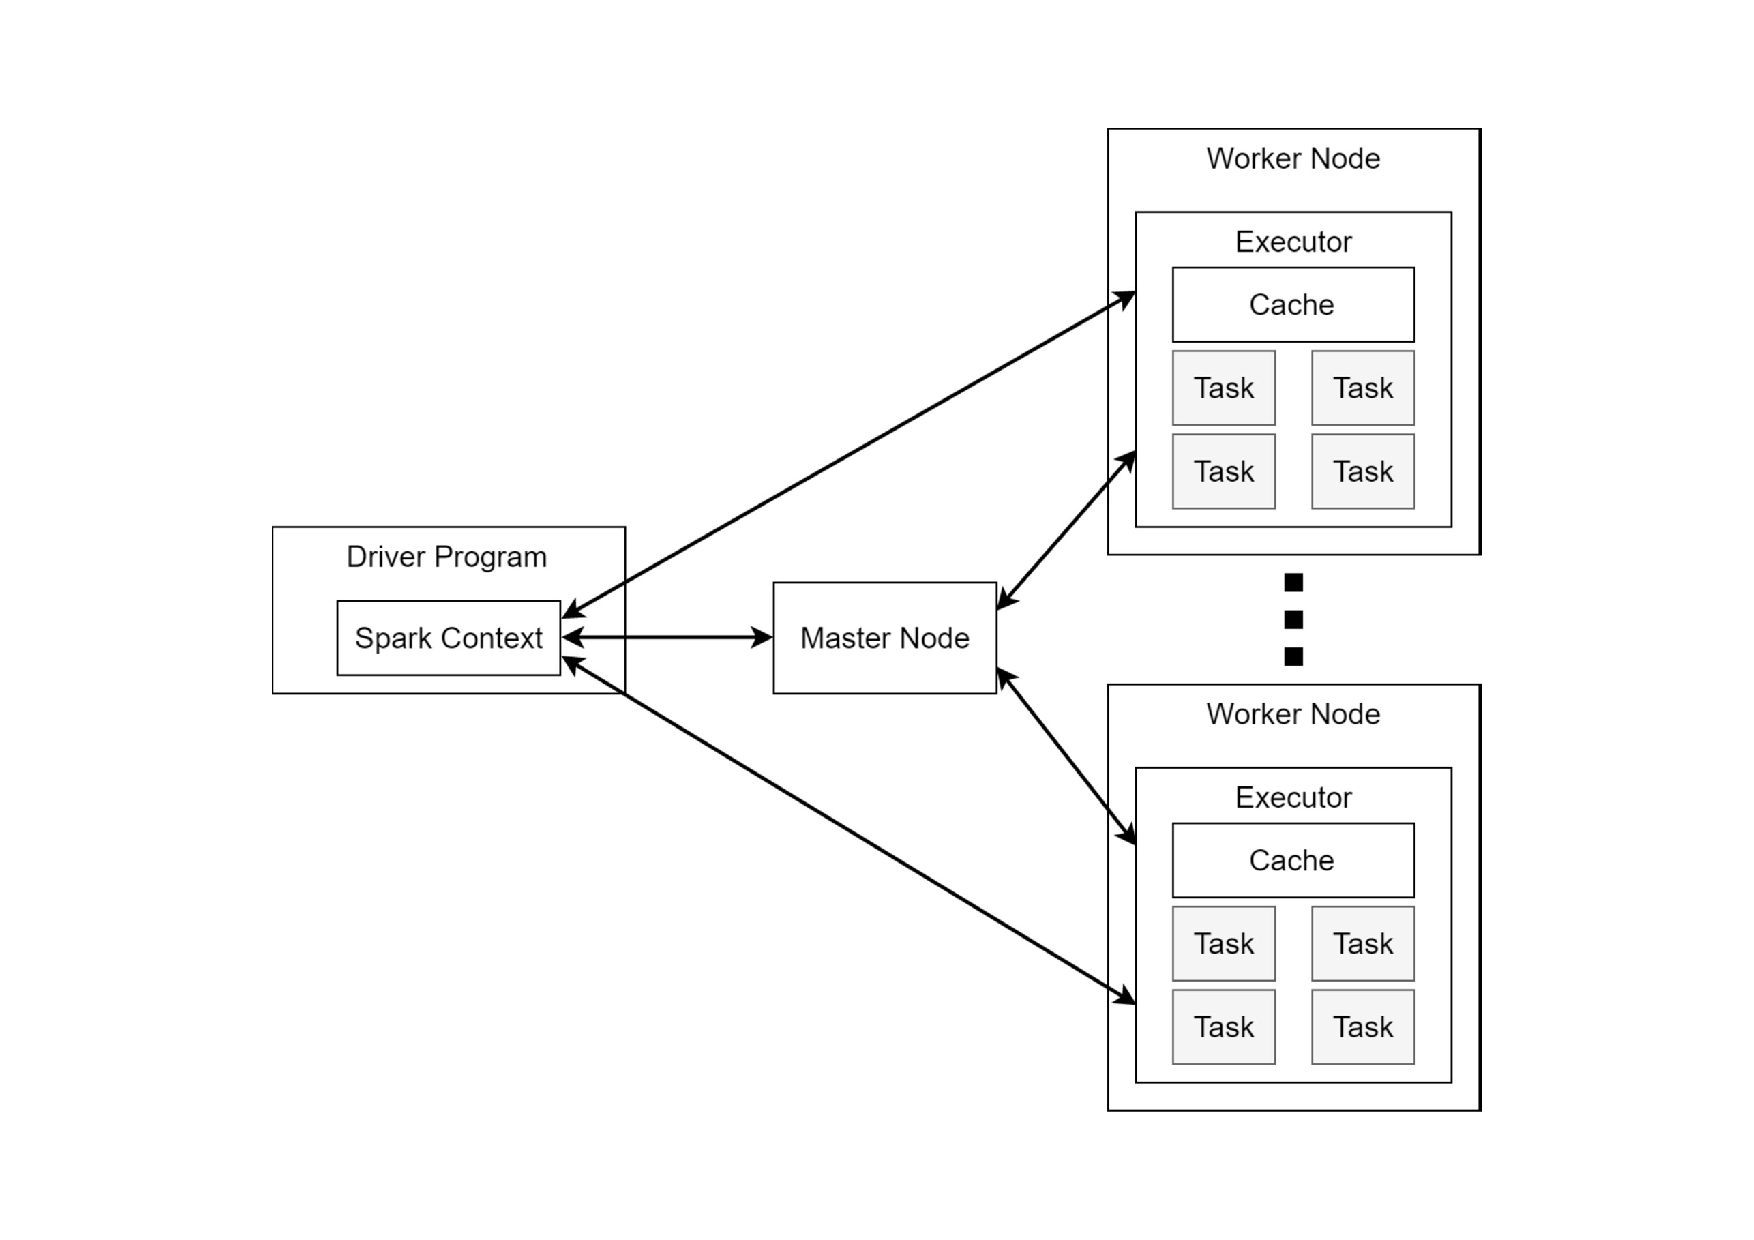
\includegraphics[width=\columnwidth]{Images/spark_standalone_architecture.pdf}  
	\caption[Spark Standalone Architecture]{Spark Standalone Architecture.}
	\label{fig:sparkStandaloneArchitecture}
\end{figure}

Different high-level libraries have been developed in order to simplify
the creation of programs that can run in Spark framework.
\begin{itemize}
	\item SQL and DataFrames: support for relational queries, that are the most common data processing paradigm
	\item Spark Streaming: implements incremental stream processing using a model called "discretized streams", input data is split into micro batches
	\item GraphX: graph computation interface
	\item MLlib: machine learning library, more than 50 common algorithms for distributed model training
\end{itemize}
Spark architecture follows the master/worker paradigm (\myFig{fig:sparkStandaloneArchitecture}). A master server accepts data and processing request, split them into smaller chunk of data and simpler actions that can be handled
in parallel by the multiple workers. A Spark application is executed inside a driver program, that makes the user code executable on the computing cluster using a SparkContext. The driver program is responsible for managing the job flow and scheduling tasks that will run on the executors. The SparkContext will split the requested operations in tasks the can be scheduled for distributed execution on
the workers. When a SparkContext is created, a new Executor process is created on each worker. An executor is a separate Java Virtual Machine (JVM) that runs for the entire lifetime of the Spark application, executes tasks using a thread pool and store data for its Spark application. Communication between the SparkContext and the other
components is performed using a shared bus.
\begin{figure}
	\centering
	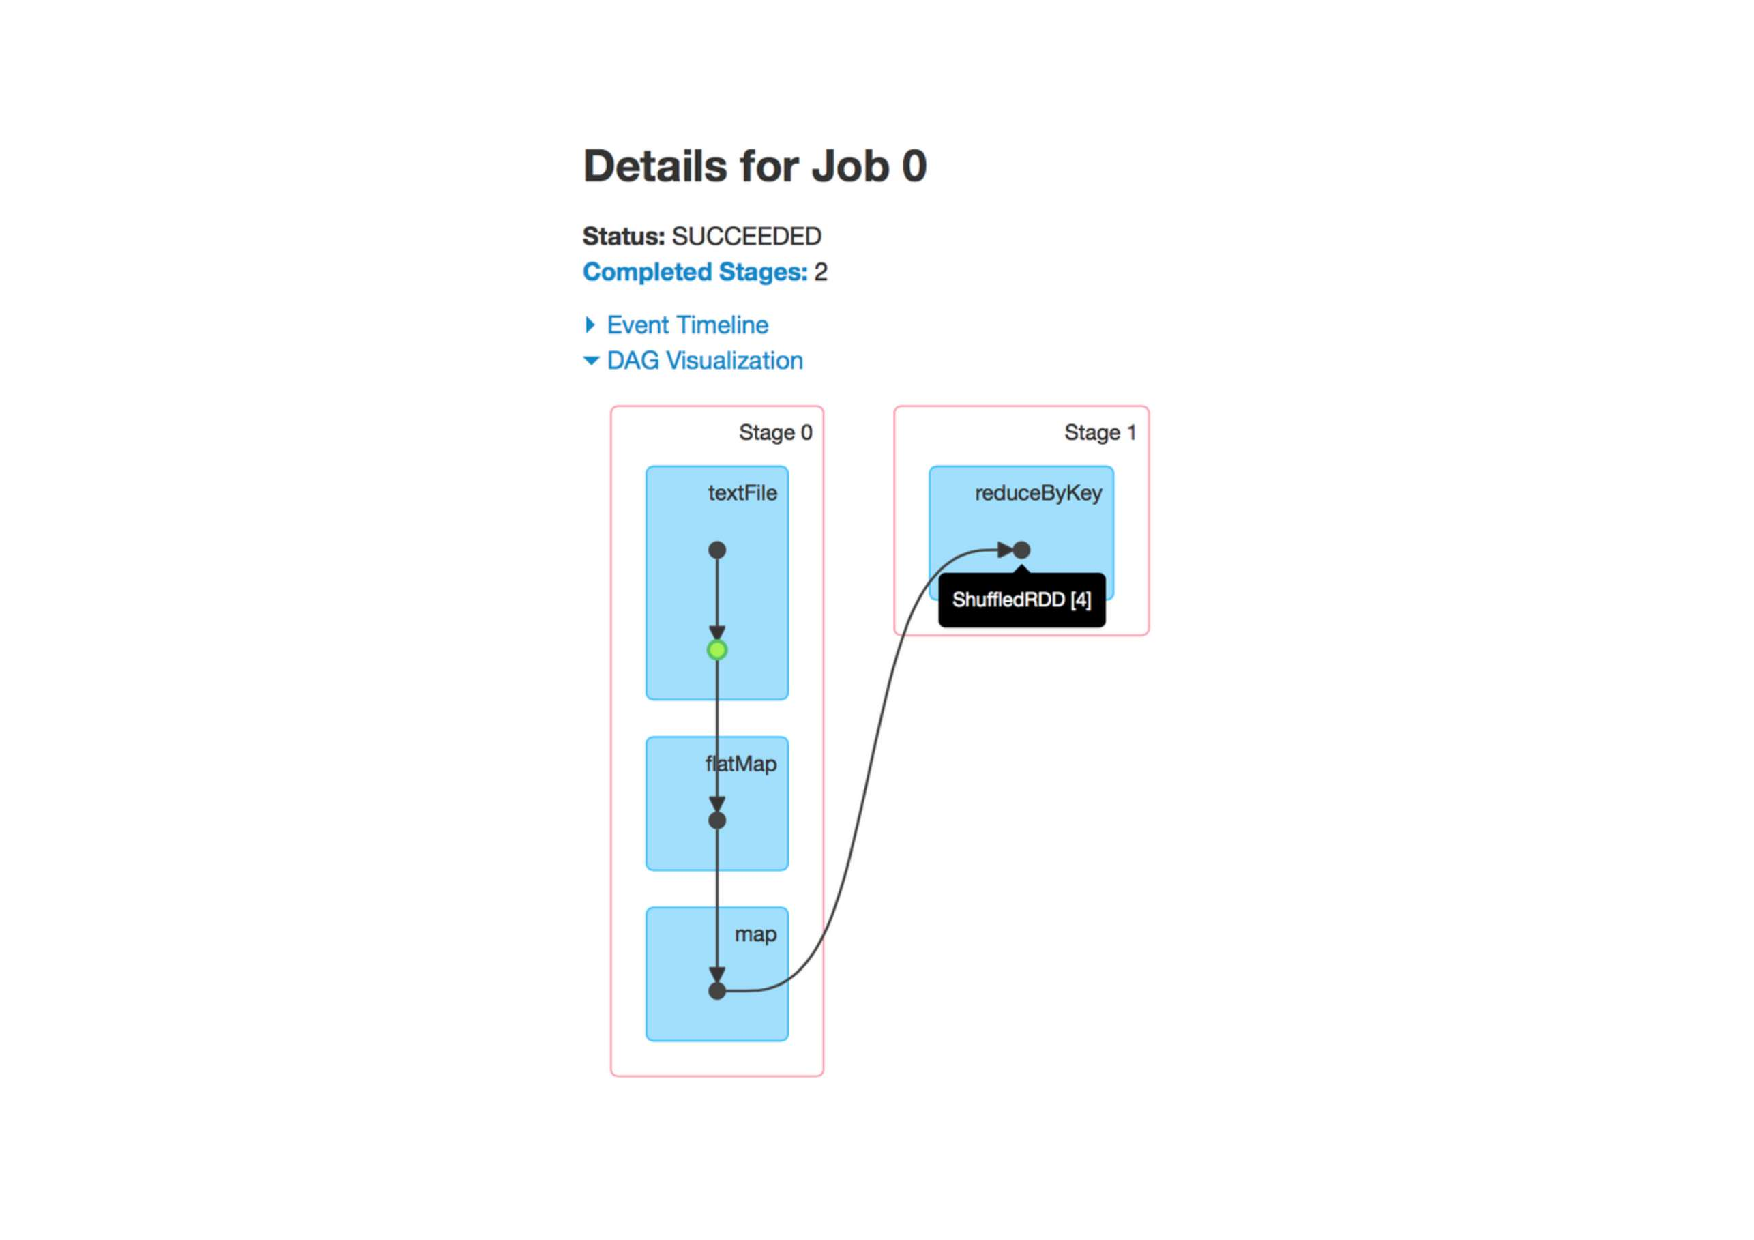
\includegraphics[width=\columnwidth]{Images/spark_dag_example.pdf}  
	\caption[Spark DAG Example]{Spark DAG Example.}
	\label{fig:sparkDAGExample}
\end{figure}
When an application is submitted to Spark, it is divided in multiple jobs. Jobs are delimited by Spark actions in the application code. Spark actions are those operations that return a value to the driver program after running a computation on the dataset.
For each job, a Directed Acyclic Graph (DAG) is created to keep track of the RDDs that are materialized inside the job. DAG nodes represent the RDDs, meanwhile arcs represent transformations, that are the operations that create new datasets from existing ones.
The application steps inside a single job are further organized into stages, that are delimited by operations require data reshuffling, that will inevitably break locality.  Spark distinguishes between narrow transformations, that do not reshuffle data (e.g., map, filter), and wide transformations, that require data reshuffling (e.g., reduceByKey). Stages are also used to produce intermediate result that can be persisted
to memory or mass storage to avoid re-computation. When all stages inside a job
have been identified, Spark can determine which parallel tasks need to be executed for each stage, and schedule them for operation on the executors. Spark creates one task for each partition of the RDD received in input by a stage.

\lstinputlisting[
firstline=1,
lastline=4,
float=tb,
language=Java,
tabsize=2,
numbers=left,
numberstyle=\tiny,
stepnumber=1,
numbersep=5pt,
caption={Spark word count application example.}, 
captionpos=t,
label=lst:wordCount
]{CodeFiles/wordCount.java}

In \MyFig{fig:sparkDAGExample}, we can see a simple DAG representing the single job
of the word count application presented in \MyListing{lst:wordCount} \cite{misc:SparkApplication}. The image was obtained from SparkWeb UI. Through a textFile operation, the input file is read from HDFS. Then a flatMap operation is applied to split each of the lines of the document into words. Following, another
map is used to create (’word’, 1) pairs. Finally, a reduceByKey operation is performed  to count the occurrences of each word. The blue boxes represent the Spark operations that the user calls in his code, while the dots represent the RDDs that are created as a result of these operations. Operations are grouped into stages, represented by the boxes with a red border. The job has been divided into two stages because the reduceByKey transformation requires the data to be shuffled. The green dot represents a cached RDD, in particular the data read from HDFS has been cached, in this way future computations on this RDD can be done faster since data will be read from memory instead of HDFS. The default deployment of Spark is in standalone mode, that is using its embedded cluster manager. 

\subsection{Streams Processing: Flink}\label{sec:flink}
\begin{figure}
	\centering
	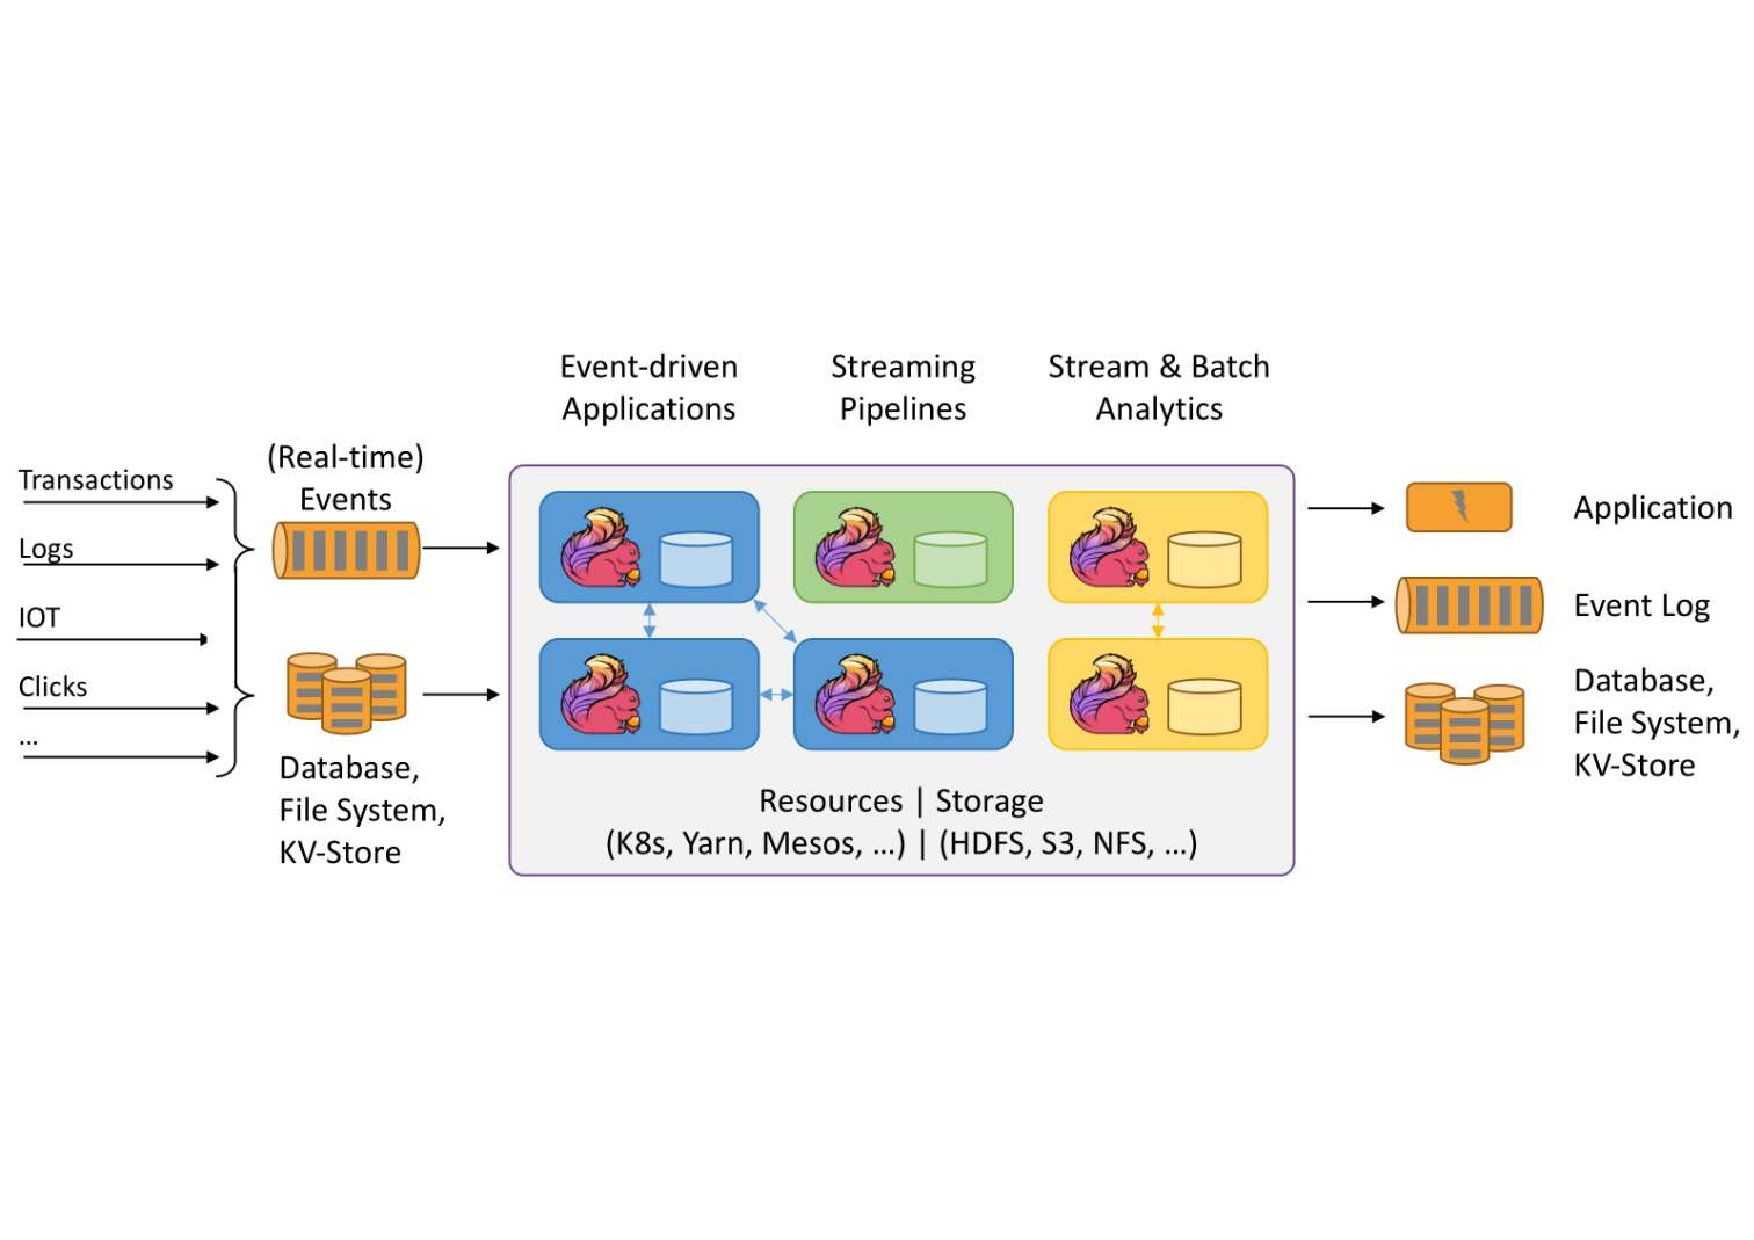
\includegraphics[width=\columnwidth]{Images/apache_flink.pdf}
	\caption[Apache Flink® - Stateful Computations over Data Streams.]{Apache Flink® - Stateful Computations over Data Streams.}
	\label{fig:apache_flink}
\end{figure}
\begin{figure}
	\centering
	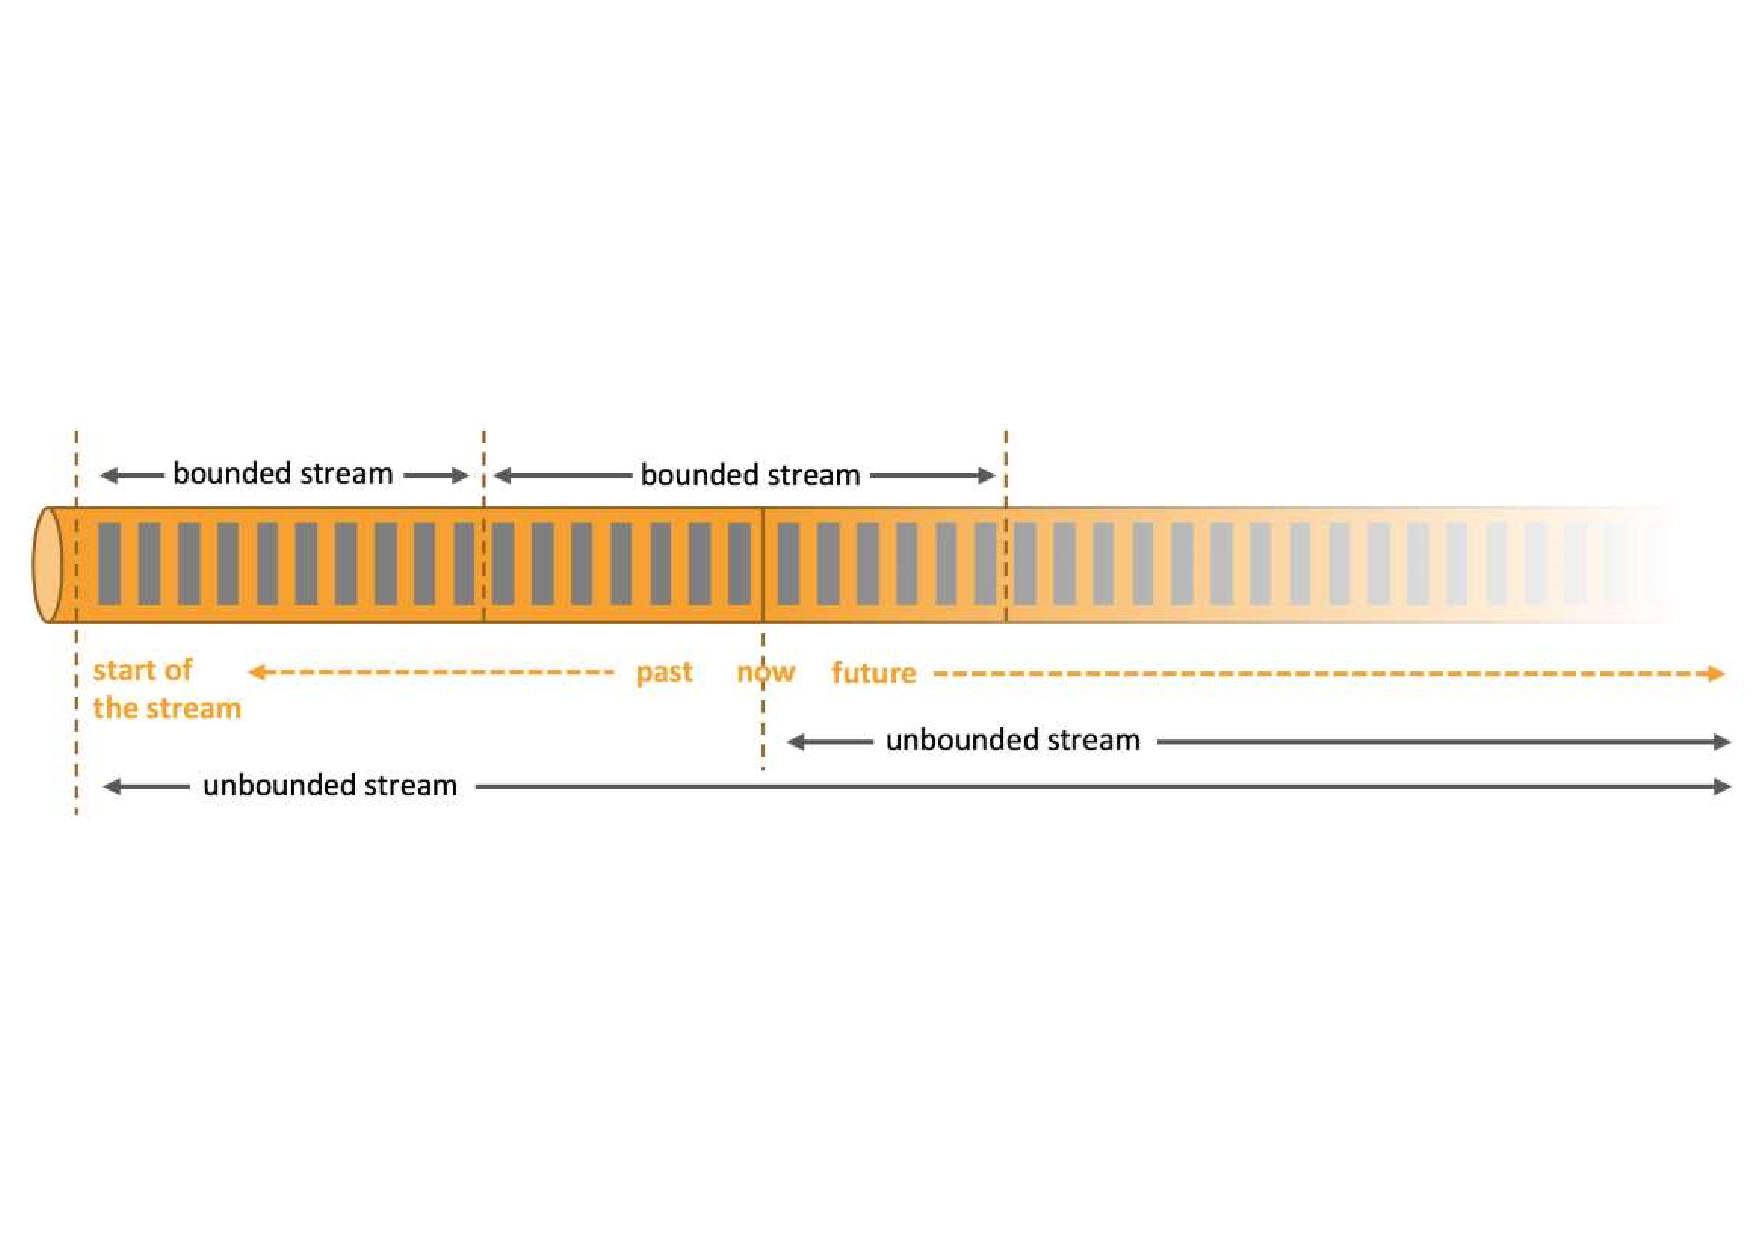
\includegraphics[width=\columnwidth]{Images/apache_flink_data_streams.pdf}
	\caption[Apache Flink® - Bounded \& Unbounded Data Streams.]{Apache Flink® - Bounded \& Unbounded Data Streams.}
	\label{fig:apache_flink_data_streams}
\end{figure}

Apache Flink~\cite{misc:ApacheFlink} is a framework and distributed processing engine for stateful computations over unbounded and bounded data streams. It can run in any commonly used cluster environments, computes at in-memory speed and manages data at any scale.

Flink’s architecture is suitable for processing unbounded and bounded data. Any type of data is generated as a stream of events. Sensors data, server logs or user interactions on a website or mobile application, credit card transactions, all of these data are generated as streams of data.

Data can be processed as unbounded or bounded streams~\cite{misc:ApacheFlinkArchitecture}. 

Unbounded streams have a start but no defined end. They do not terminate and provide data as it is generated. Unbounded streams must be continuously processed, i.e., events must be promptly handled after they have been ingested. It is not possible to wait for all input data to arrive because the input is unbounded and will not be complete at any point in time. Processing unbounded data often requires that events are ingested in a specific order, such as the order in which events occurred, to be able to reason about result completeness.

Bounded streams have a defined start and end. Bounded streams can be processed by ingesting all data before performing any computations. Ordered ingestion is not required to process bounded streams because a bounded data set can always be sorted. Processing of bounded streams is also known as batch processing.


Apache Flink excels at processing unbounded and bounded data sets. Precise control of time and state enable Flink’s runtime to run any kind of application on unbounded streams. Bounded streams are internally processed by algorithms and data structures that are specifically designed for fixed sized data sets, yielding excellent performance.

\subsection{Streams Processing: Storm}\label{sec:storm}

\begin{figure}
	\centering
	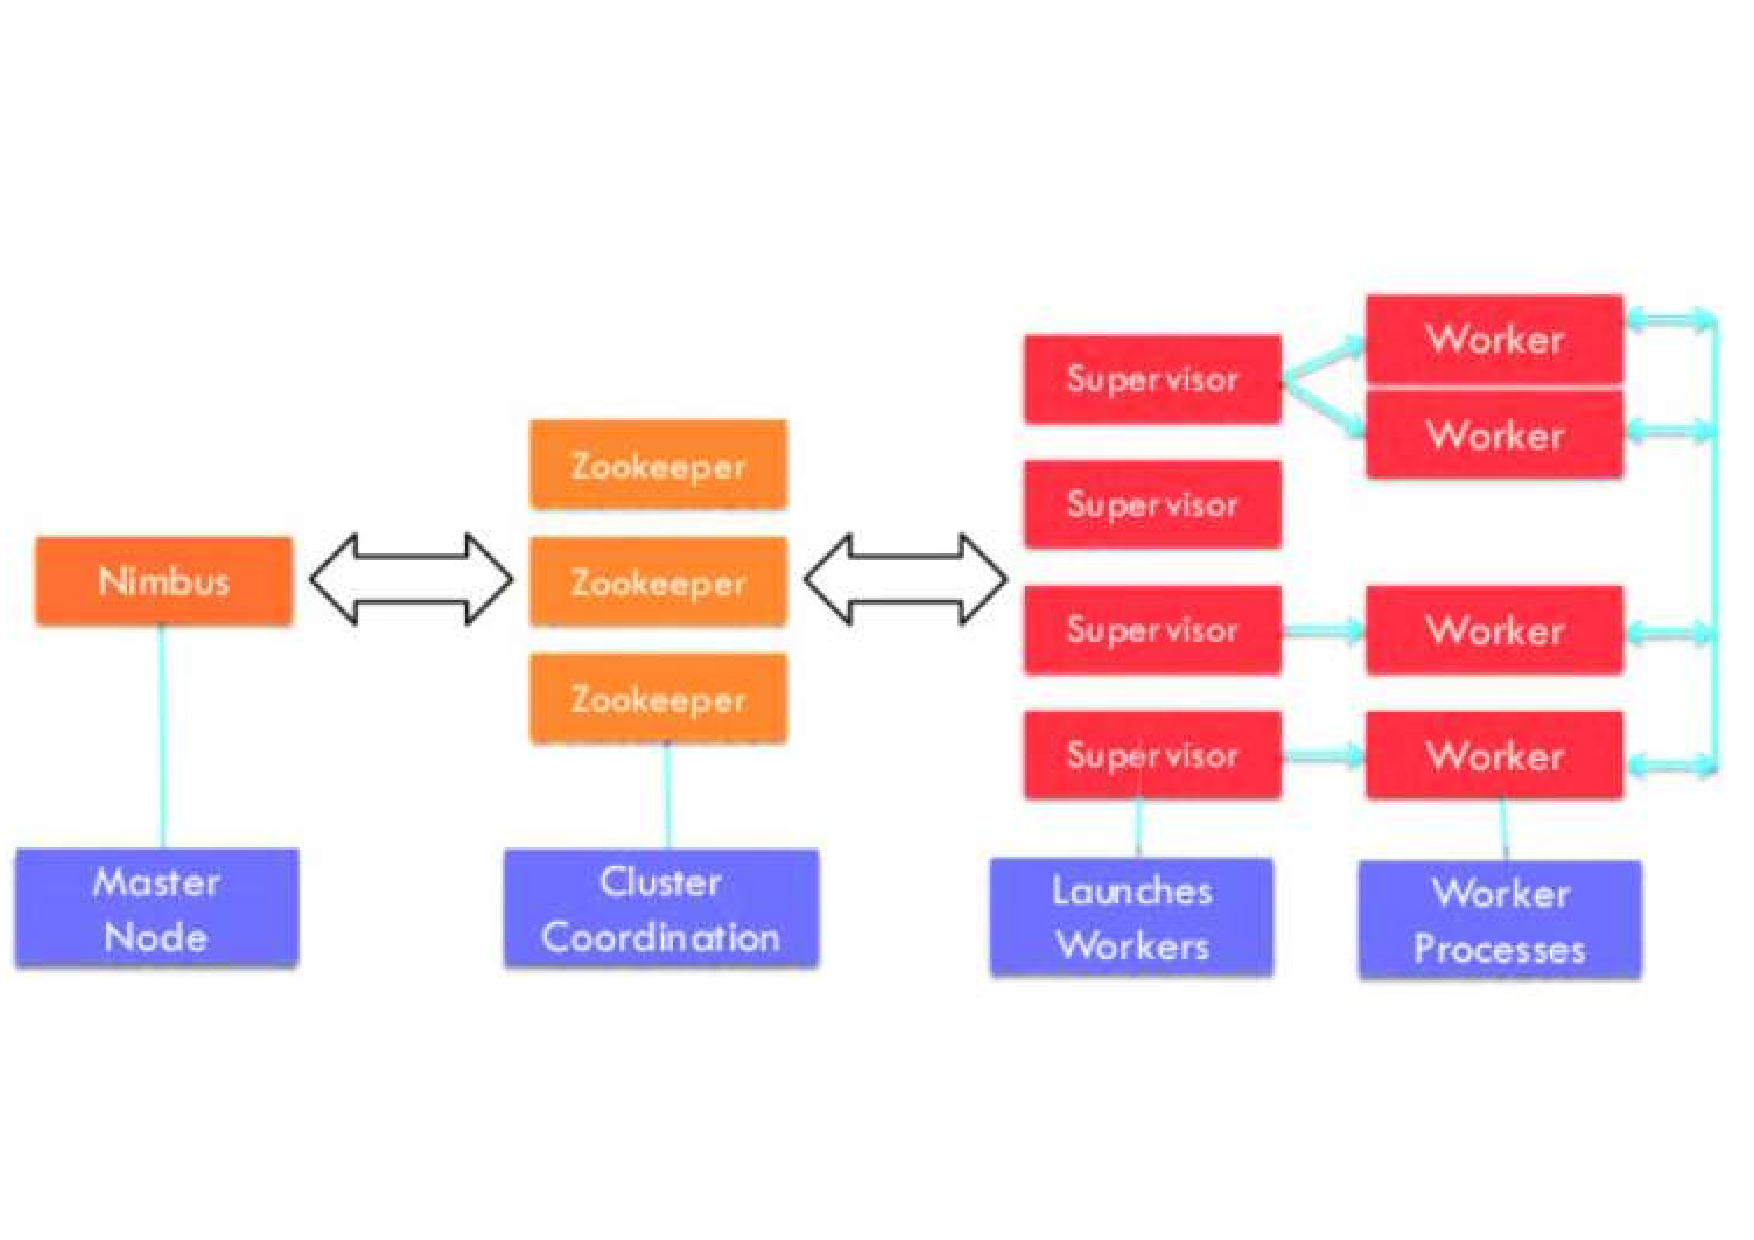
\includegraphics[width=\columnwidth]{Images/apache_storm.pdf}
	\caption[Apache Storm.]{Apache Storm.}
	\label{fig:apache_storm}
\end{figure}
\begin{figure}
	\centering
	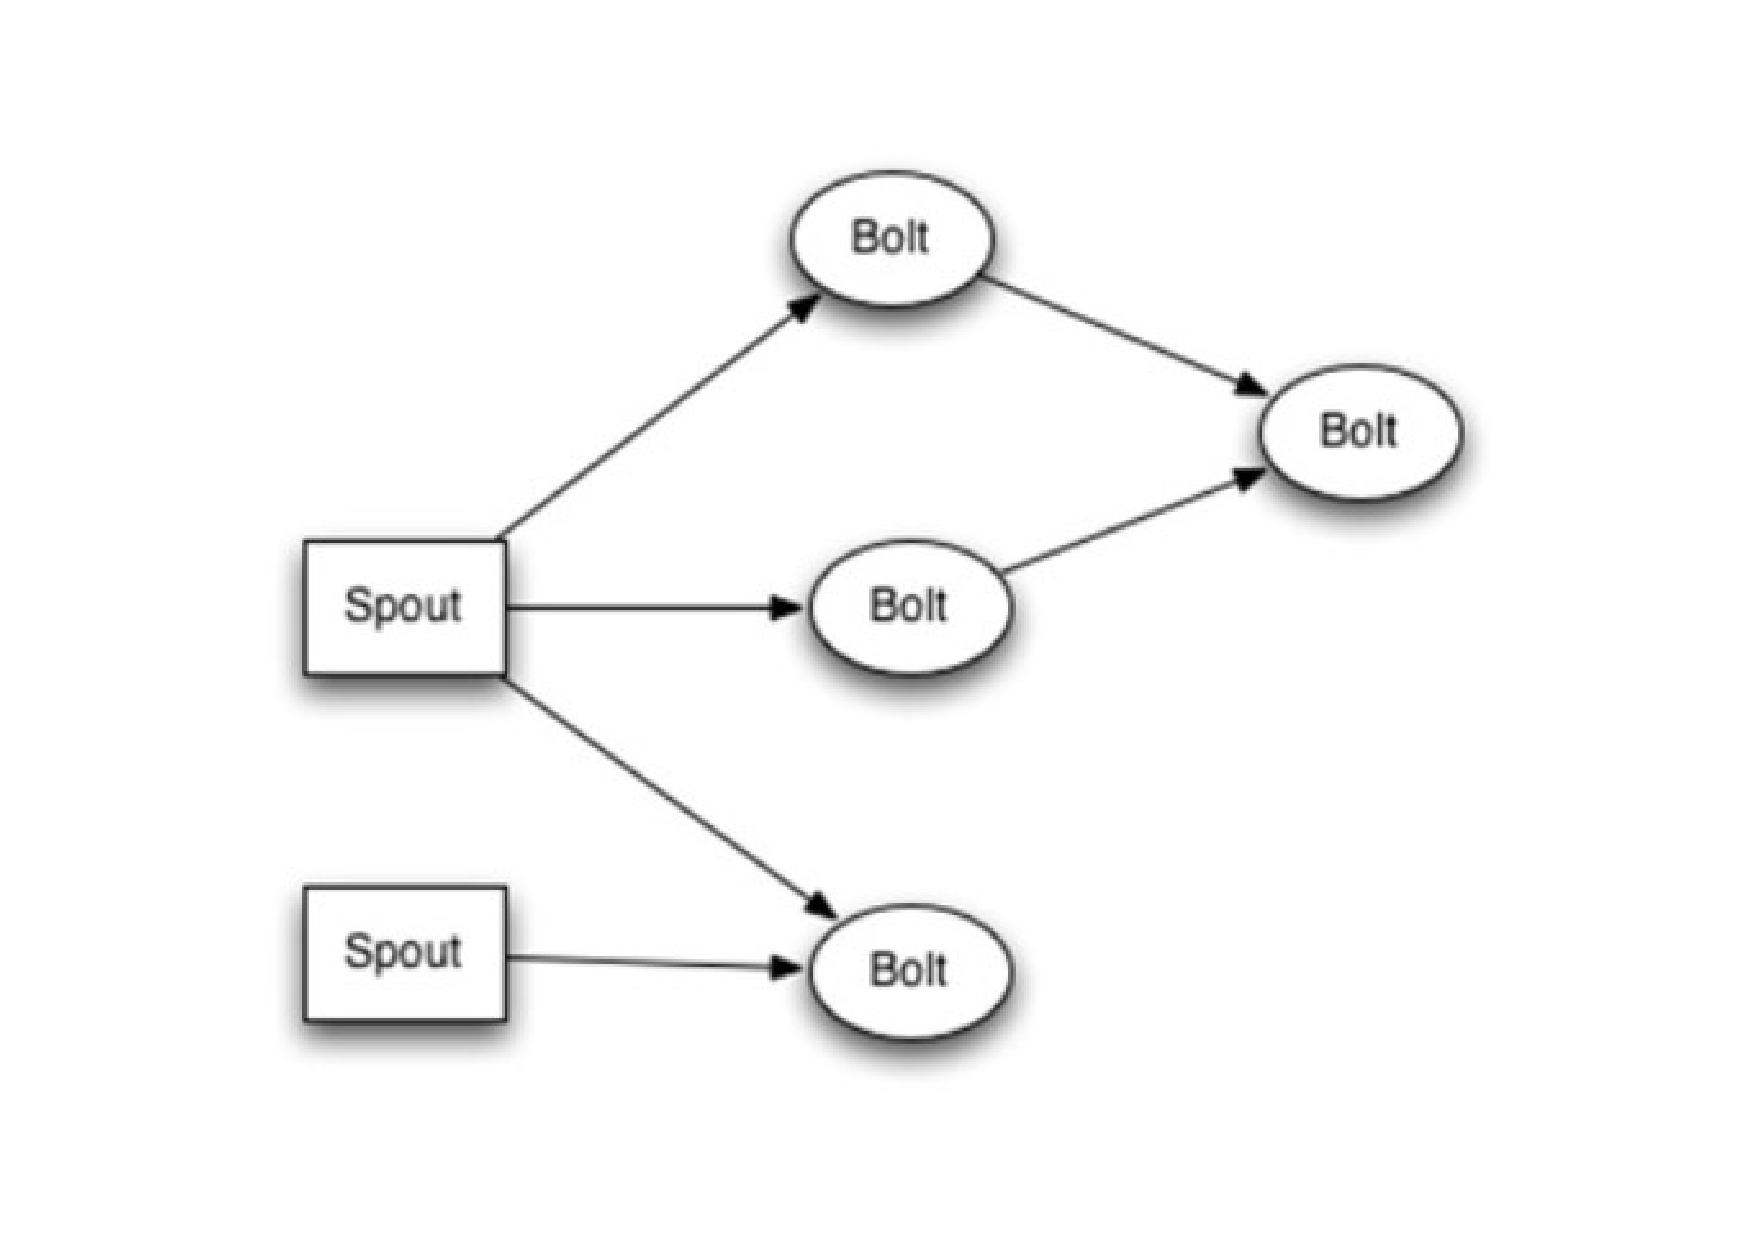
\includegraphics[width=\columnwidth]{Images/apache_storm_components_abstraction.pdf}
	\caption[Apache Storm Components Abstraction.]{Apache Storm Components Abstraction.}
	\label{fig:apache_storm_components_abstraction}
\end{figure}

Apache Storm~\cite{misc:ApacheStorm} is a free and open source distributed realtime computation system. Storm makes it easy to reliably process unbounded streams of data, doing for realtime processing what Hadoop did for batch processing. Storm is simple, can be used with any programming language, and is easy to use.

Storm has many use cases: realtime analytics, online machine learning, continuous computation, distributed RPC, ETL, and more. Storm is fast: a benchmark clocked it at over a million tuples processed per second per node. It is scalable, fault-tolerant, guarantees your data will be processed, and is easy to set up and operate.

Storm integrates with the queueing and database technologies you already use. A Storm topology consumes streams of data and processes those streams in arbitrarily complex ways, repartitioning the streams between each stage of the computation however needed. 

The Apache Storm architecture is quite similar to that of Hadoop. However there are certain differences which can be better understood by getting a closer look at its cluster in \MyFig{fig:apache_storm}: 
\textbf{Nodes} - There are two types of nodes in Storm cluster similar to Hadoop:
\begin{itemize}
	\item {Master node - }The master node of Storm runs a daemon called ‘Nimbus’, which is similar to the ‘Job Tracker’ of Hadoop cluster. Nimbus is responsible for distributing codes, assigning tasks to machines and monitoring their performance.
	\item {Worker node – }Similar to the master node, the worker node also runs a daemon called ‘Supervisor’ which is able to run one or more worker processes on its node. Each supervisor works assigned by Nimbus and starts and stops the worker processes when required. Every worker process runs a specific set of topology which consists of worker processes working around machines. Since Apache Storm does not have the abilities to manage its cluster state, it depends on \textbf{Apache Zookeeper} for this purpose. Zookeeper facilitates communication between Nimbus and Supervisors with the help of message acknowledgements, processing status, etc.
\end{itemize}
\textbf{Storm Components/Abstractions} (see  \MyFig{fig:apache_storm_components_abstraction}) – There are basically four components which are responsible for performing the tasks:

\begin{itemize}
	\item Topology – Storm Topology can be described as a network made of \textbf{spouts} and \textbf{bolts}. It can be compared to the Map and Reduce jobs of Hadoop. Spouts are the data stream source tasks and Bolts are the accrual processing tasks. Every node in the network consists of processing logic’s and links to demonstrate the ways in which data will pass and the processes will be executed. Each time a topology is submitted to the storm cluster, Nimbus consults the supervisor nodes about the worker nodes. 
	\item Stream – One of the basic abstractions of the storm architecture is stream which is an unbounded pipeline of tuples. A tuple can be defined as the fundamental component in the Storm cluster containing a named list of the values or elements.  \item Spout – It is the entry point or the source of streams in the topology. It is responsible for getting in touch with the actual data source, receiving data continuously, transforming those data into actual stream of tuples and finally sending them to the bolts to be processed. two types of nodes in Storm cluster.
	\item Bolt - Bolts keep the logic required for processing. These are responsible for emitting the streams for processing by other bolts and saving or sending the data for storage. These are capable of running functions, filtering tuples, aggregating and joining streams, linking with database, etc.
\end{itemize}

\section{Runtime Management of Big Data Applications}\label{sec:runtime_mgmt_big_data_apps}
Big data applications requires system scalability, fault tolerance and  availability~\cite{articleBigData:2017}. 

\textit{Scalability} means the ability to maintain an approximate linear relationship between the size of processed data and the amount of consumed resources. 

\textit{Fault tolerance} is a challenge, especially when systems are complex and involve many networked nodes. By means of hardware virtualization, cloud computing services satisfies all the requested requisites, and the \textit{elasticity} and redundancy it provides  also enable big data application high availability, scalability and fault tolerance.

Another very important feature of big data applications is the \textit{Quality of Service} or \qos.

\qos definition for IT applications differ by application type. Interactive applications are usually assessed according to response time or throughput, and their fulfillment depends on the intensity and variety of the incoming requests. 

Big data applications might require a single batch computation on a very large dataset, thus \qos must consider the execution of a single run. In this domain \qos is often called \textit{deadline}, or the desired duration of the computation. 

We have mentioned availability, fault tolerance and availability as fundamental requirements and \qos as a measure of the capability to meet a user-defined deadline when processing big data. Many factors influence the duration of an application execution, surely resource allocation greatly influences the duration. 

The challenges introduced by big data require resilient, flexible and self-adapting software systems~\cite{DeLemos2013}. Hence, \textit{autonomic system}s and \textit{self-adaptation} has increasingly captured the attention of researchers ~\cite{Weyns:2012:CSE:2666795.2666811}. These systems automatically react to changes in the environment, or in their own state, and change their behaviour to satisfy functional and non-functional requirements. Meeting requirements in complex and variable execution environments is a difficult task that can be tackled at design time or at runtime. At runtime the adaptation is very often obtained by using a well-known process called MAPE~\cite{MAPE}, a control loop composed of four phases: monitoring, analysis, planning and execution.

One of the challenges that modern software systems face is the provisioning and optimization of resources to meet a varying demand, generated by are increasingly common phenomena like fluctuating workloads, unpredictable peaks of traffic and unexpected changes. Service providers cannot disregards these factors if they want to cope with the challenge of satisfying functional and non-functional requirements, usually defined in SLAs (Service Level Agreements). Hence the need arises for an automatic adjustment of system resources allocation to avoid resource saturation and unresponsiveness, users dissatisfaction and unnecessary costs. This paradigm is called elastic resource provisioning~\cite{Dustdar2011, Zhang2010, Sehgal2012, Herbst2013}.

Many approaches about elastic systems and dynamic resource allocation were proposed both in the industry and in academia. In modern technology elasticity is often enabled by cloud computing that gives to an application a theoretical infinite degree of scalability. However considering only resources is rather restrictive because of the many factors that impact application during their runtime life-cycle. In fact Dustdar et al.~\cite{Dustdar2011} argue that elastic computing should be designed by considering three dimensions: quality, resources and cost.  Quality elasticity considers how quality is affected by a change in resource availability. Instead cost elasticity measures how resource provision is affected when a change in cost happens. 

Cloud computing services provide the needed level of fault tolerance and availability required by big data applications. In the remainder of this chapter we present an overview of popular big data frameworks that can leverage cloud computing solutions and how they address elastic resource allocation to satisfy functional and non-functional application requirements. The resulting scenario represent the base for our work, where we will consider quality elasticity and not cost elasticity aspects. 

This thesis shows how the application of lightweight symbolic execution tecniques to deadline-based \qos constrained multi-DAG big data applications helps reduce the number of deadline violations and allocate resources more efficiently.


\section{Elastic Resource Provisioning}
\label{Section:Introduction:ElasticProvisioning}

The word \textit{elasticity} comes from physics and is defined as the ability of an object or material to resume its normal shape after being stretched or compressed. In computing, elasticity has a similar meaning and is used to characterize \textit{autonomic systems}. Herbst et al.~\cite{Herbst2013} defines elastic provisioning as reported below.
\begin{quote}
	\textit{\textbf{Elasticity} is the capability of a system to adapt to workload changes by provisioning or de-provisioning resources automatically such that at each point in time the available resources match the current demand as closely as possible}.
\end{quote}

A system is in an \textit{under provisioned} state if it allocates less resources than required by the current demand; it is in an \textit{over provisioned} state if allocates more resources than required. Moreover, elasticity is determined by four attributes:

\begin{itemize}
	\item \textit{Autonomic Scaling}: the adaptation process used to control the system.
	\item \textit{Elasticity Dimensions}: the set of scaled resources in the adaptation process.
	\item \textit{Resource Scaling Units}: the minimum amount of allocable resources to each dimension.
	\item \textit{Scalability Bounds}: the lower and the upper bound on the amount of resources that can be allocated to each dimension.
\end{itemize}

Additionally, two aspects must be considered in evaluating the elasticity degree of a system: speed and precision. 

\textbf{Speed of scaling up/down:} the time it takes to switch from an underprovisioned/overprovisioned state to an optimal or overprovisioned/underprovisioned state respectively. 

\textbf{Precision of scaling}: the absolute deviation of the current amount of allocated resources from the actual resource demand.

Scalability and efficiency are terms related to elasticity, nevertheless they differ by the following aspects:
 
\textbf{Scalability}, although is a prerequisite for elasticity, it does not consider the temporal aspects (how fast and how often) and the granularity of the adaptation actions.

\textbf{Efficiency}, contrary to elasticity, it takes in account all the types of resources employed to accomplish a certain amount of work, not only the resources scaled by the adaptation actions. 

\begin{figure}
	\centering
	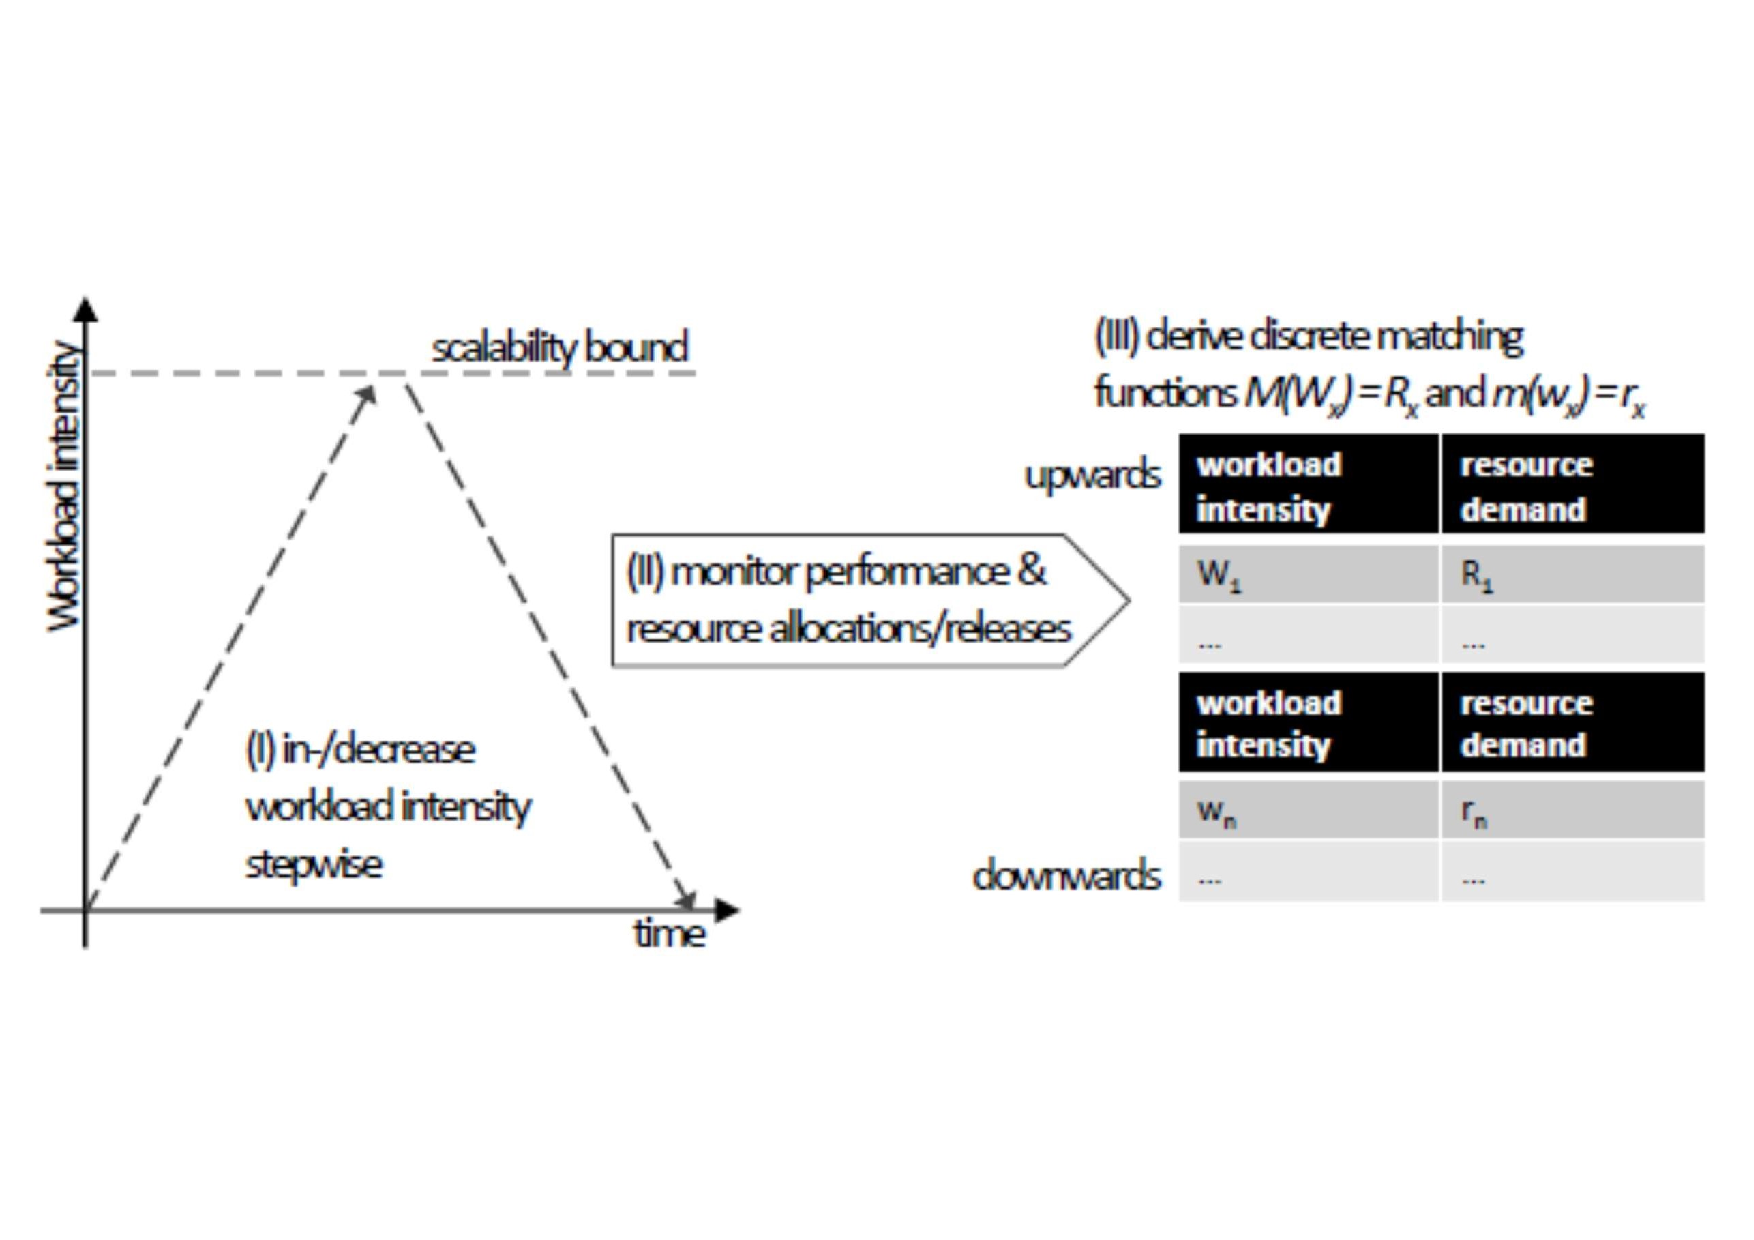
\includegraphics[width=\columnwidth]{Images/elasticity_matching_function.pdf}
	\caption[Elasticity Matching Function derivation.]{Elasticity Matching Function derivation.}
	\label{fig:elasticity_matching_function}
\end{figure}
\begin{figure}
	\centering
	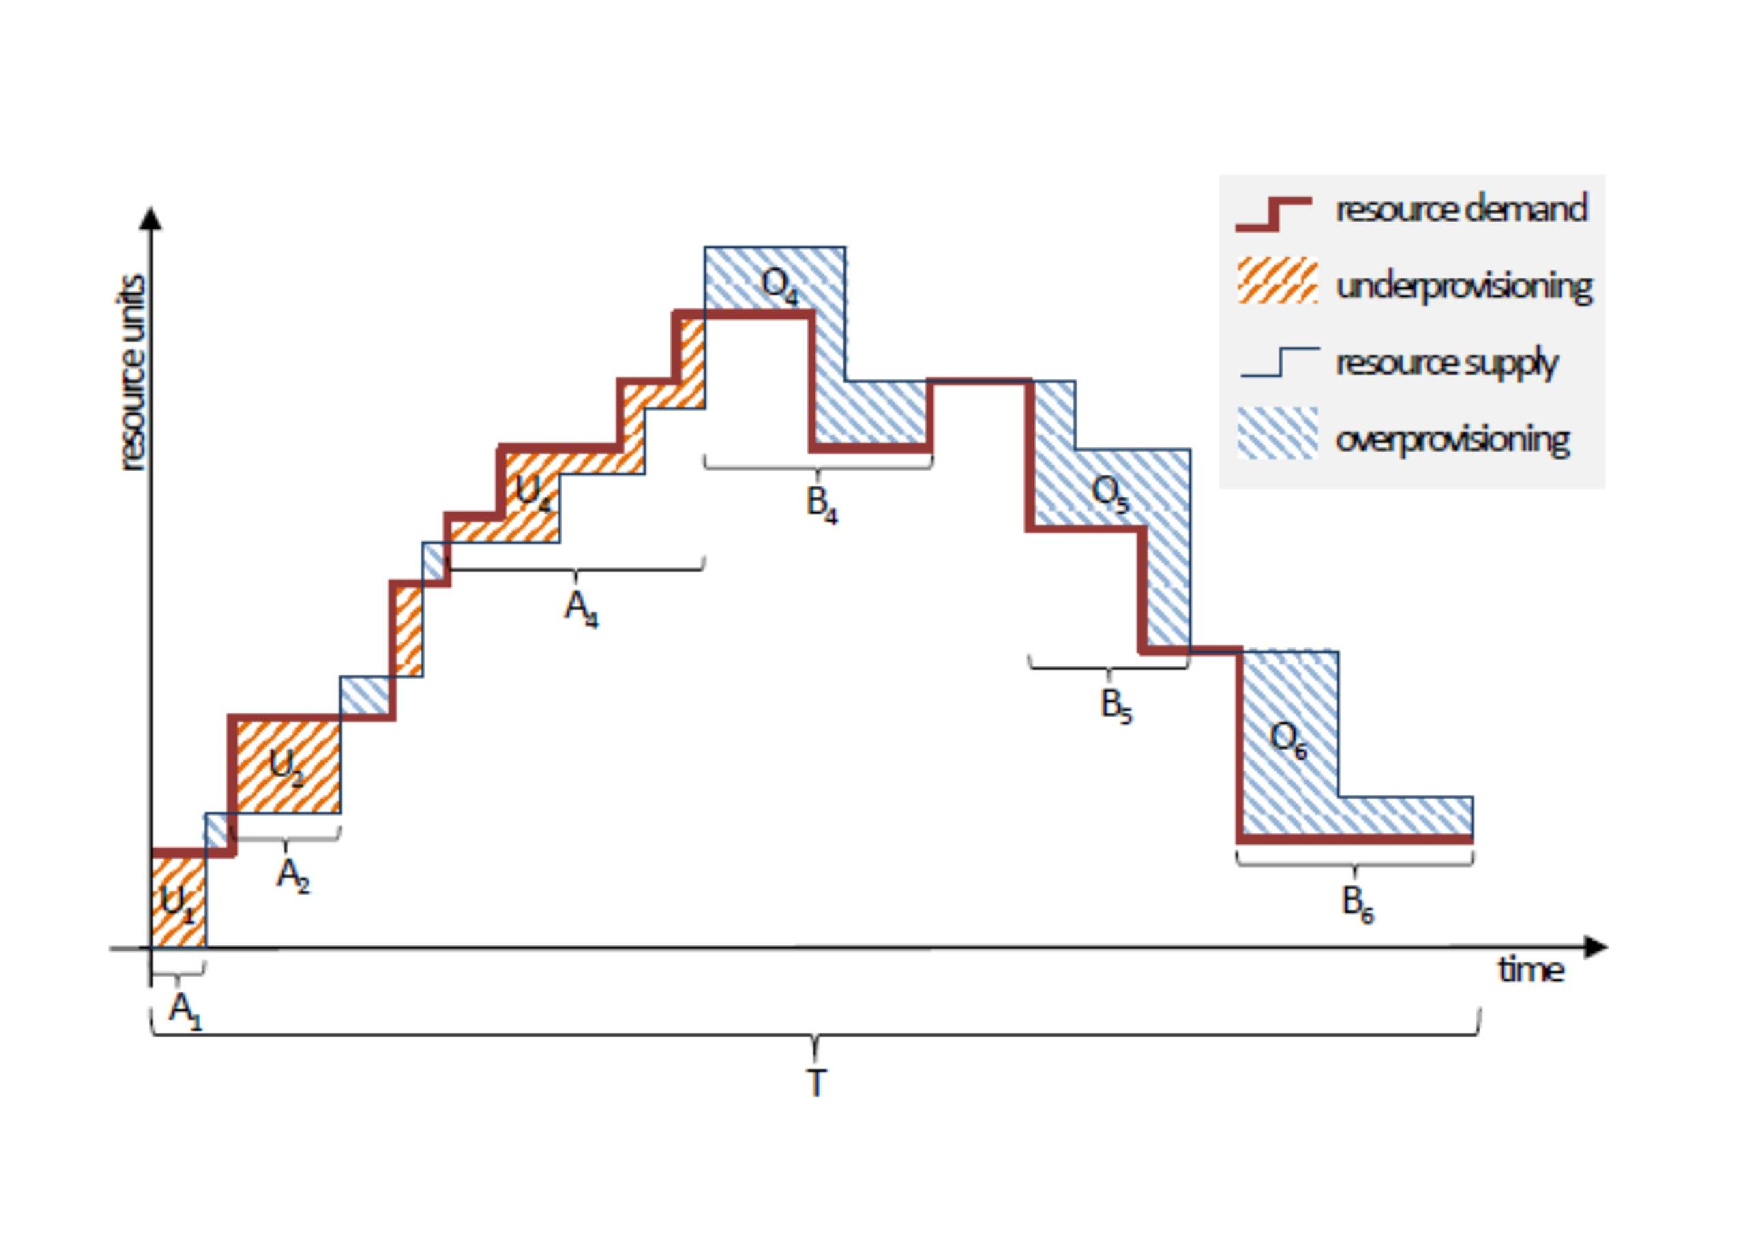
\includegraphics[width=\columnwidth]{Images/elasticity_resource_provisioning_chart.pdf}
	\caption[Resource Provisioning Chart.]{Resource Provisioning Chart.}
	\label{fig:elasticity_resource_provisioning_chart}
\end{figure}

Elasticity reflects the (theoretical) infinite upper bound on resource scalability in cloud computing and the frictionless resource renting model. Nevertheless elasticity is not just a synonym of resource management. Elasticity is also related to trade off between cost and quality~\cite{Dustdar2011}. Cost elasticity describes how resources are managed in response to cost changes, while quality elasticity measures how responsive is the quality to changes in resource utilization.

A \textit{matching function} $m(w) - r$ is a system specific function that gives the minimum quantity of resources r for any given resource type needed to meet the system’s performance requirements at a certain workload intensity. A matching function is required for both up and down scaling directions.

The matching functions can be determined based on measurements, as illustrated in \MyFig{fig:elasticity_matching_function}, by increasing the workload intensity w stepwise, and measuring the resource consumption r, while tracking resource allocation changes. The process is then repeated for decreasing w. After each change in the workload intensity, the system should be given enough time to adapt its resource allocations reaching a stable state for the respective workload intensity. As a rule of thumb, at least two times the technical resource provisioning time is recommended to use as a minimum. As a result of this step, a system specific table is derived that maps workload intensity levels to resource demands, and the other way round, for both scaling directions within the scaling bounds.

An example of how \textit{speed} and \textit{precision} affect resource provisioning is shown in \MyFig{fig:elasticity_resource_provisioning_chart}.


\section{Spark Resource Provisioning}\label{sec:spark_resource_provisioning}
It's important to remember that the cluster manager is responsible for starting executor processes and determine where and when they will run. Using Spark’s embedded cluster manager might be a problem in terms of resource utilization when we want to execute different distributed applications at the same time. Using a single cluster manager for different distributed applications has the advantage of providing a global view on which applications are running and which we want to execute inside the cluster.
Without a single cluster manager, we can have two main approaches
in order to perform resource sharing and allocation:
\begin{itemize}
	\item  allowing every application to allocate all the resources in the cluster at the same time, this leads to an unfair situation of resource contention
	\item splitting the resource pool into smaller pools, one per application.
\end{itemize}
In this way we will avoid resource contention but we will
have a less efficient utilization of the resources, because some of
the applications might request more resources than the ones in
the pool, meanwhile some others are using less resources than
the allocable ones in order to execute.
A more dynamic way of allocating resources will lead to a better resource
utilization. Spark natively support executing on top of Apache
Hadoop YARN and Apache Mesos cluster managers.
Spark supports the dynamic allocation of executors, also known as
elastic scaling, this feature allows to add and remove Spark executors
in a dynamic way in order to match the workload.
In traditional static allocation, a Spark application would allocate
CPU and memory upon starting the execution, disregarding how
much resources will effectively use later on. With dynamic allocation
instead it is possible to allocate as much resources as they are
necessary, in order to avoid wasting them. The number of running
executors is scaled up and down according to the workload, in particular
idling executors are removed and when there are tasks waiting
to be executed and new executors are launched. Dynamic allocation can 
be activate in Spark settings and should be used together with the
External Shuffle Service, in this way data that have been manipulated
from the executor is still available after the removal of the executor.
Dynamic allocation has two different policy for scaling the executors:
\begin{itemize}
	\item Scale Up Policy: new executor are requested when there are
	pending tasks, the number of executors is increased exponentially
	because they start slow and so the application might need
	a slightly higher number of them
	\item Scale Down Policy: idling executors are removed after a certain
	amount of time, this amount of time can be configured
\end{itemize}
In order for dynamic allocation to work, we must configure it, by setting
the initial number of executors that are created when application
starts and the minimum and maximum number of executors that can
be reached when scaling down and up respectively. Dynamic allocation
is available on all cluster managers currently supported by Spark,
even in Standalone mode.

\subsection{Apache Hadoop Yarn}\label{sec:hadoop_yarn}
Apache Hadoop YARN (Yet Another Resource Negotiator) is the next
generation of Hadoop’s compute platform\cite{Vavilapalli:2013:AHY:2523616.2523633}. 
\begin{figure}
	\centering
	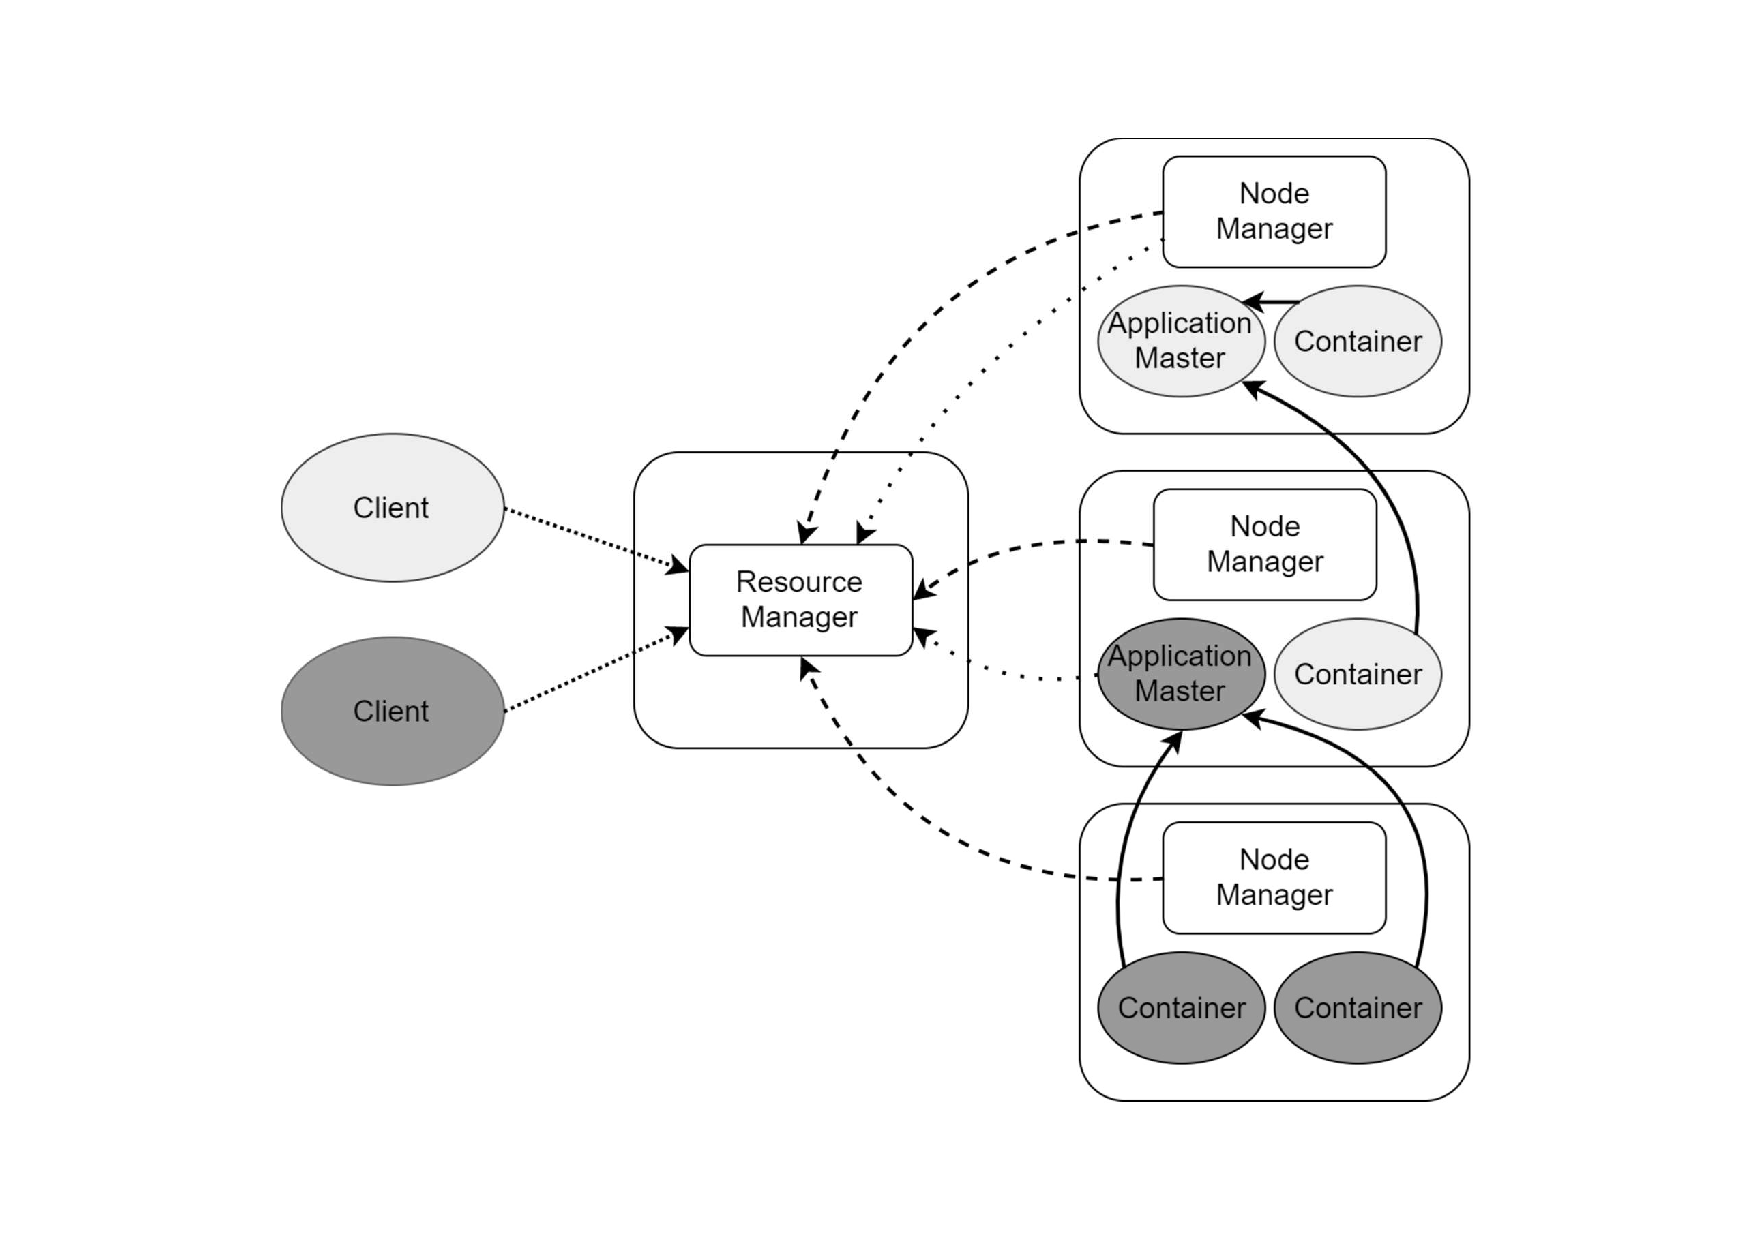
\includegraphics[width=\columnwidth]{Images/apache_hadoop_yarn_architecture.pdf}  
	\caption[Apache Hadoop YARN Architecture]{Apache Hadoop YARN Architecture.}
	\label{fig:apacheHadoopYarnArchitecture}
\end{figure}
The idea is to split
the functionality of resource management and job scheduling and
monitoring. This is achieved by having two different kind of daemons
running, one global Resource Manager (RM) and a per-application
Application Master (AM).
Resource Manager (RM) and Node Manager (NM) form the data
computation framework (Figure 1.4). RM is the authority that manages
resources among all the applications that are running in the
system, meanwhile NM is the per-machine daemon who is responsible
for managing containers, monitoring and reporting. The perapplication
AM has the goal of negotiating resources with RM and
working with NM in order to execute and monitor tasks.
Resource Manager (RM) is composed by two components: Scheduler
and Applications Manager.
The Scheduler is responsible for allocating resources to the various
applications that are running, by taking into account constraints
about capacity, queues, etc. It is a real scheduler in the sense that
it does not perform monitoring or tracking of the application state.
Moreover, it does not offer any guarantee that a failed application will be reexecuted
after an application or hardware failure. The Scheduler performs
the allocation according to the resources that are requested by
an application; this is based on the abstract notion of container which
has elements as memory, CPU cores, disk and network bandwidth.
There are pluggable policy that determine the repartition of resources
among the different applications, for example we have the Capacity
Scheduler, designed for multi-tenant clusters, and the Fair Scheduler,
that shares cluster resources fairly.
The Applications Manager is responsible of accepting the submission
of a job, it negotiates the first container that will execute the AM and
it offers a service that can be used to restart the AM in case of failure.
The per-application AM has the goal of negotiating the needed
containers from the Scheduler, track their status and monitor their
progress.
The RM keeps a global model of the cluster state and thanks to the
resource requirements reported by the running applications, it makes
possible to enforce a global scheduling, but it is required to have an
accurate understanding of the applications’ resource requirements. In
response to AM requests, the RM generates containers together with
tokens that grant access to resources. An extension of the protocol
allows the RM to ask back resources from applications, for example
when cluster resources become scarce.
Application Master (AM) is the process that coordinates the execution
of an application inside the cluster. It is important to remember
that AM itself is run in the cluster, just like any other container. Periodically,
an heartbeat is sent to the RM in order to confirm its liveliness
and to update the Scheduler about its resource requests. After having
modeled the application requirements, the AM encodes its preferences
and constraints inside the heartbeat message. This information
are stored in the form of Resource Request, containing the desired number of containers (e.g., 100 container), the resources of each container
(e.g., <2 CPU, 2 GB>), the locality preferences and the priority of this
resource request with respect to the other ones of this application.
When a container lease is received, the AM can choose to modify its
execution plan in order to take into account the abundance or scarcity
of resources.
Node Manager (NM) is the worker daemon in YARN, its purpose
is to authenticate container lease, manage dependencies, monitoring
the execution of containers and offer them a set of services. After
having registered with the RM, the NM sends heartbeats in order to
communicate its status and receives instructions from the RM. All
the containers are described by a container launch context (CLC), that
keeps track of all the environment variables, the dependencies, the security
tokens, but also of the payloads needed by NM services and the
commands that are needed to launch the process inside the container.
After having validated the authenticity of the container lease, the NM
configures the container with the specified resource constraints and
initializes a monitoring subsystem. In order to launch the container,
dependencies are copied into local storage. NM also has the duty of
killing container upon a request from RM or AM, for example when a
tenant is being evicted or when an application completes. Whenever
a container exits, NM needs to clean the working directory. When an
application ends, all the resources held by its container on all nodes
are released. NM periodically checks the state of the physical machine
and informs the RM of a possible unhealthy state.
\subsection{Apache Mesos}\label{sec:apache_mesos}
Apache Mesos is an open-source project used to manage computer
clusters. 
\begin{figure}
	\centering
	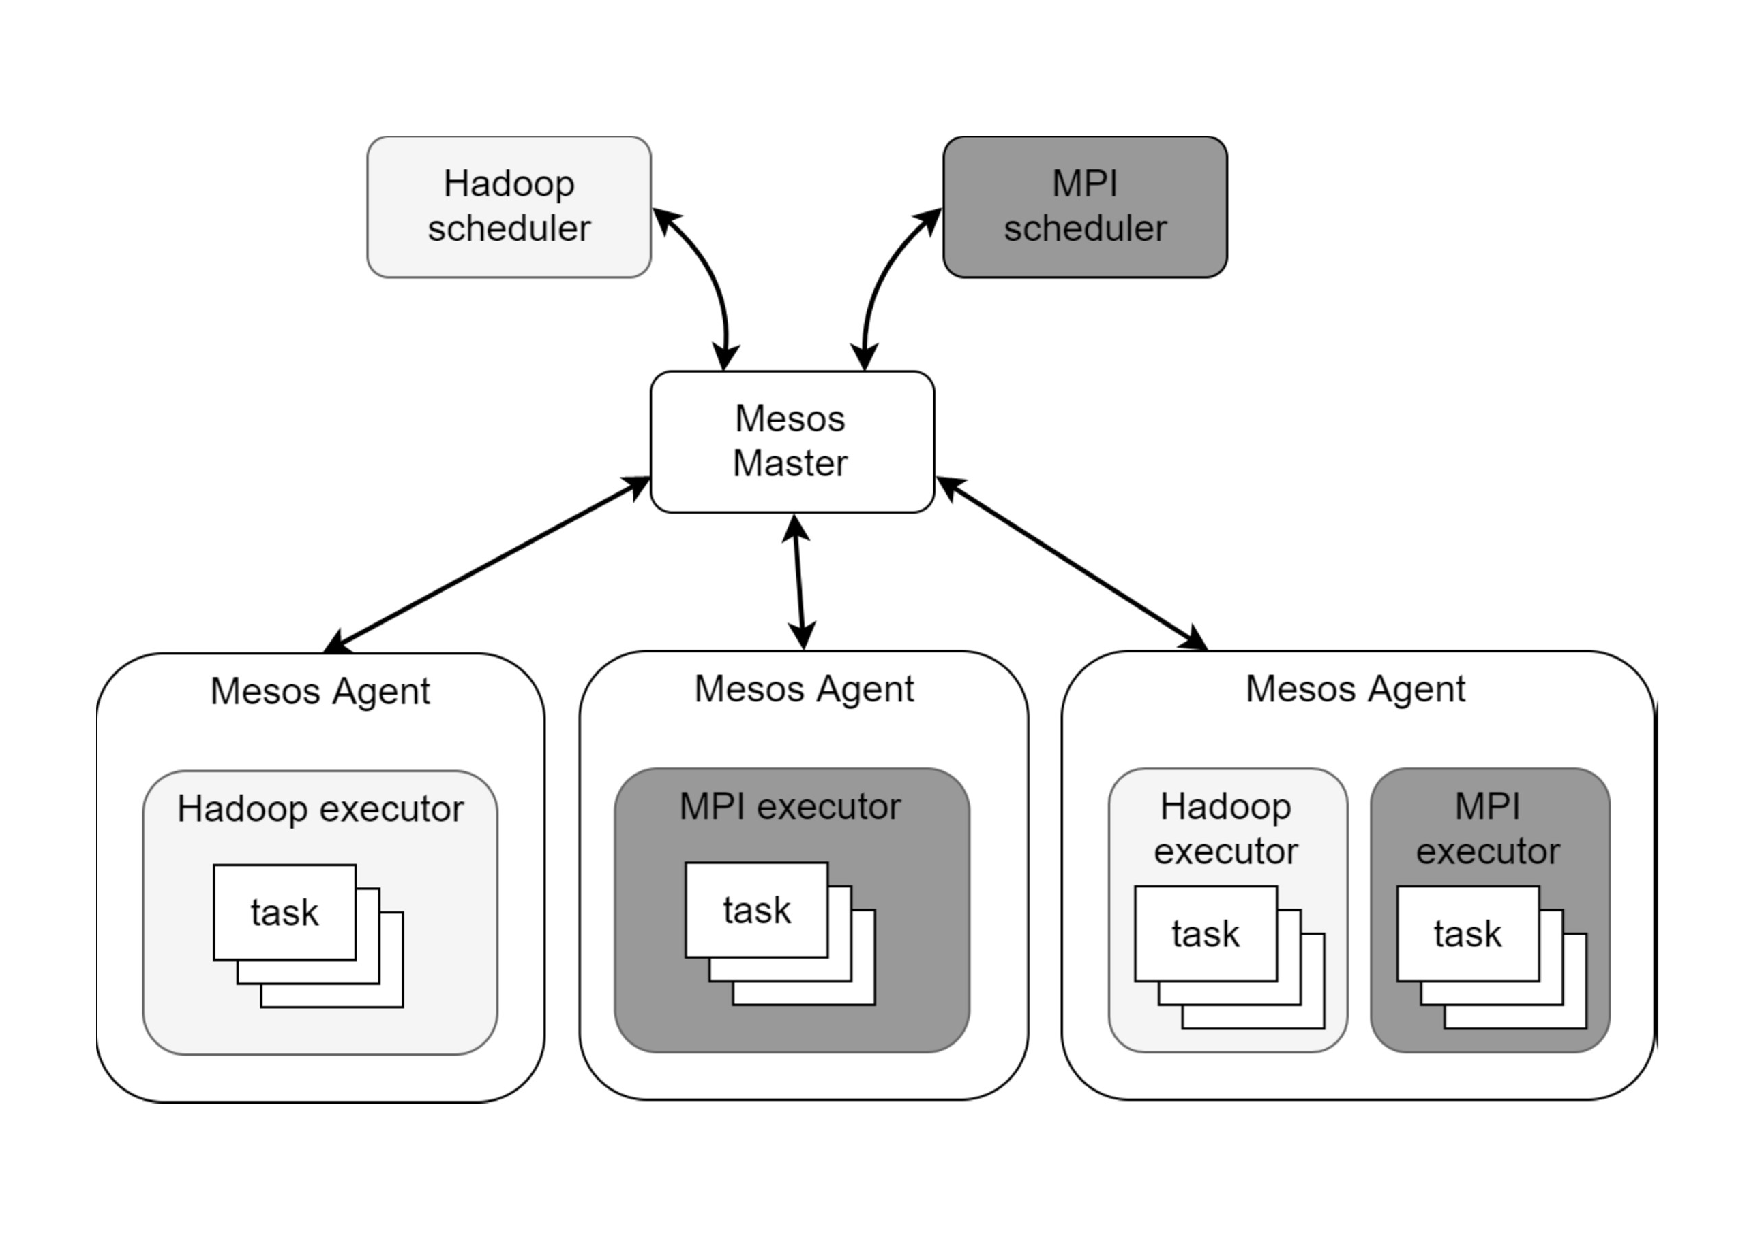
\includegraphics[width=\columnwidth]{Images/apache_mesos_architecture.pdf}  
	\caption[Apache Mesos Architecture]{Apache Mesos Architecture.}
	\label{fig:apacheMesosArchitecture}
\end{figure}
The purpose of Mesos is to share cluster between different
computing frameworks, such as Apache Hadoop or Message Passing
Interface (MPI). The sharing increments the utilization of the cluster
and prevents per-framework data replication. 
Mesos shares resources
in a fine-grained way, allowing to achieve data locality. It presents
a scheduling mechanism on two layer called resource offers. Mesos
decides how many resources to offer to each of the running frameworks,
meanwhile they decide how many resources to accept and
which computation to execute on the granted resources.
New cluster computing frameworks continue to emerge, it is clear
that finding a framework that is optimal for all type of application
is almost impossible. We expect that organization would like to use
different frameworks inside the same cluster, picking the best one according
to the kind of application that they are going to execute. Two
classic solution are: i) statically partitioning the cluster and executing
one framework per partition; ii) allocate a set of VMs to each of the
frameworks. Unluckily these solution do not achieve high utilization
and efficient data sharing. The main problem is the different allocation
granularity of these solutions and the one of the existing frameworks,
for example Hadoop employs a fine grained resource sharing
model, where nodes are divided into slots and each job is composed
by short tasks that match the slots.
\begin{figure}
	\centering
	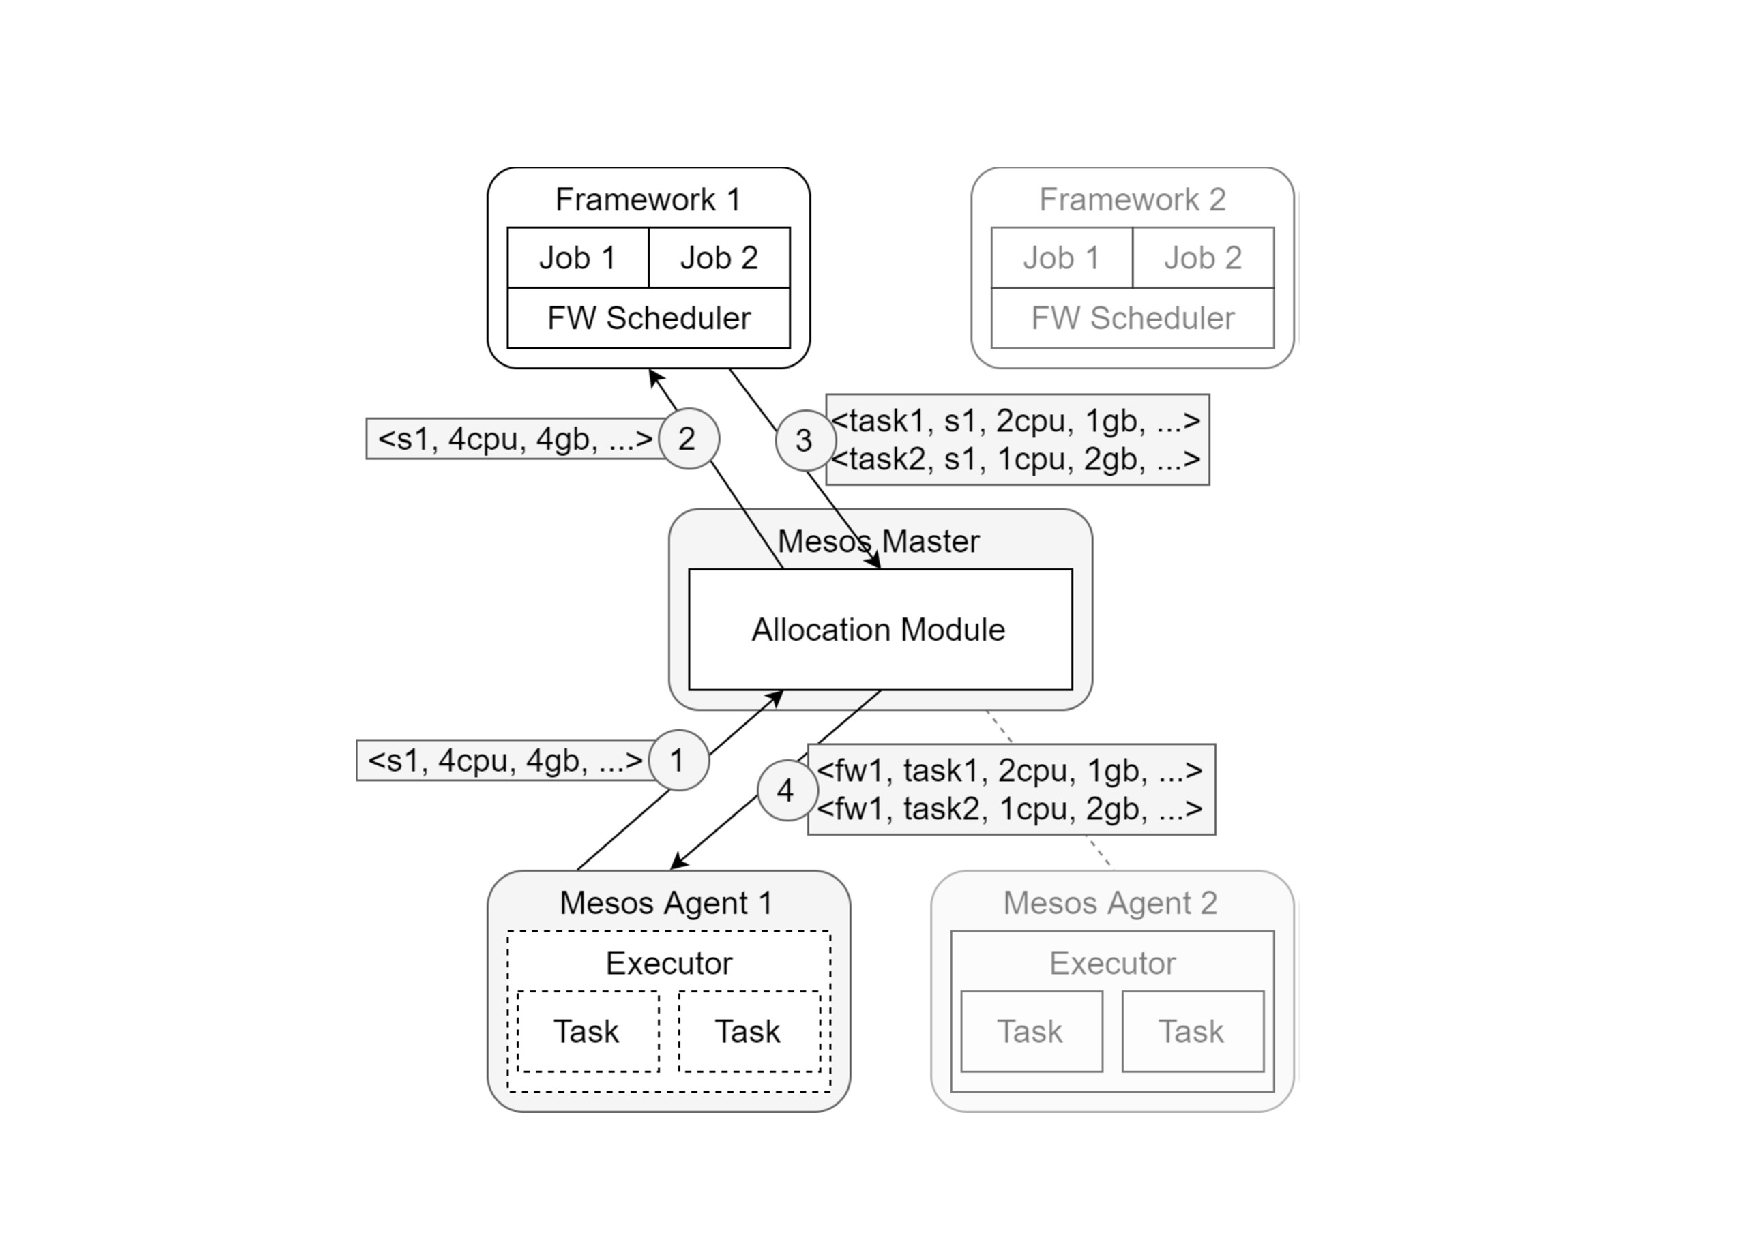
\includegraphics[width=\columnwidth]{Images/apache_mesos_resource_offer_example.pdf}  
	\caption[Apache Mesos Resource Offer Example]{Apache Mesos Resource Offer example. 1) Mesos Agent 1 reports
		free resources to the Allocation Module; 2) Allocation
		Module offers resources to Framework 1 scheduler; 3) Framework
		1 scheduler accepts resources and assign tasks; 4) Allocation
		Module launches tasks on the executor running in Mesos
		Agent 1.}
	\label{fig:apacheMesosResourceOfferExample}
\end{figure}
The presence of short tasks allows
us to achieve high utilization, as jobs can rapidly scale when
new nodes are available. But it is not possible to achieve fine grained
sharing across frameworks, because they have been developed in an
independent way, and thus it is difficult to efficiently share the cluster
among different frameworks.
Mesos delegates the control over the scheduling to the different
frameworks. In this way it is possible to have the abstraction of the
resource offers, that encapsulate a bundle of resources that the framework
can allocate on a node in order to execute a task. Mesos decides
how many resources to offer to each framework, this is based on
policies, and the framework decides which resources to accept and
which tasks to execute on them. Even though this approach does not
lead to a globally optimum scheduling, it has been proved that it performs
particularly well in practice, allowing the frameworks to obtain
near perfect data locality. Mesos provides other benefits to its users,
for example the possibility of running different instances of the same
framework or even different versions.
Mesos is composed by a master process that manages slave daemons
running on each cluster node and frameworks that run tasks
on these slaves, as we can see from \myFig{fig:apacheMesosArchitecture} . Master implements
fine-grained sharing across frameworks using resource offers. Every
resource offer is a list of free resources on the different slave nodes.
The master decides how many resources to offer to each framework,
according to some policy such as fairness or priority. 

Apache Mesos Resource Offer example. 1) Mesos Agent 1 reports
free resources to the Allocation Module; 2) Allocation
Module offers resources to Framework 1 scheduler; 3) Framework
1 scheduler accepts resources and assign tasks; 4) Allocation
Module launches tasks on the executor running in Mesos
Agent 1.

Every framework that is running on Mesos is composed by two components: a
scheduler, that registers with the master in order to obtain the resource
offers, and an executor process that is launched on the slave
node in order to execute framework’s tasks. While the master chooses
how many resources to offer, the scheduler chooses which resources
to use among those offered. When an offer is accepted, the scheduler
sends to the master the description of the tasks that should be
executed. The resource offer process is repeated every time tasks are
finished and when there are new free resources. In order to maintain
a light interface, Mesos does not ask the frameworks to specify
their resource requirements or constraint, instead it gives them the
possibility of refusing offered resources. Mesos allows frameworks to
set up a set of filters, in the form of boolean predicates, specifying
the conditions on which the framework will always refuse a proposal
(e.g., providing a whitelist of nodes it can run on).
In Figure 1.6 we have an example of resource offer process.
1. Agent 1 reports to master that it has 4 CPUs and 4 GB of memory
free. Master invokes its allocation module policy, which tells
that framework 1 should be offered all the resources.
2. Master sends a resource offer describing the resources available
on agent 1 to framework 1.


\subsection{Spark on Yarn}{subsec:sparkOnYarn}
Support for running Spark on YARN was added to Spark in version
0.6.0 and has been improved in subsequent releases~\cite{misc:SparkOnYarn}.
When running on YARN, each Spark executor is run inside a YARN
container. Spark supports two different modes to run on YARN, the
Yarn-cluster and Yarn-client mode.
In client mode, as shown in \myFig{fig:sparkOnYarnClientMode}, the driver program is run
inside the client process. In this way, the Application Master (AM) that
is run in a YARN container is used only to request resources to the Resource
Manager (RM). This mode is useful for interactive applications
and for debugging purposes, since you can see applications’ output
immediately on the client side process. If the client disconnects from
the cluster, the Spark application will terminate, this is due to the fact
that the driver process resides on the client.
In cluster mode instead, as shown in Figure 1.10, Spark driver program
is run inside the AM process managed by YARN. After initializing
the application, client can disconnect from the cluster and reconnect
later on. This mode makes sense when using Spark on YARN in
production jobs.
Running on top of YARN cluster manager has some benefits. First
of all YARN allows to dynamically share the cluster resources between
the different frameworks that are running together. For example
we can run MapReduce jobs after running Spark jobs without the
need of changing YARN configurations. Moreover, YARN supports
for categorizing, isolating and prioritizing workloads and employs
security policies, in this way Spark can use secure authentication between
its processes.
\begin{figure}
	\centering
	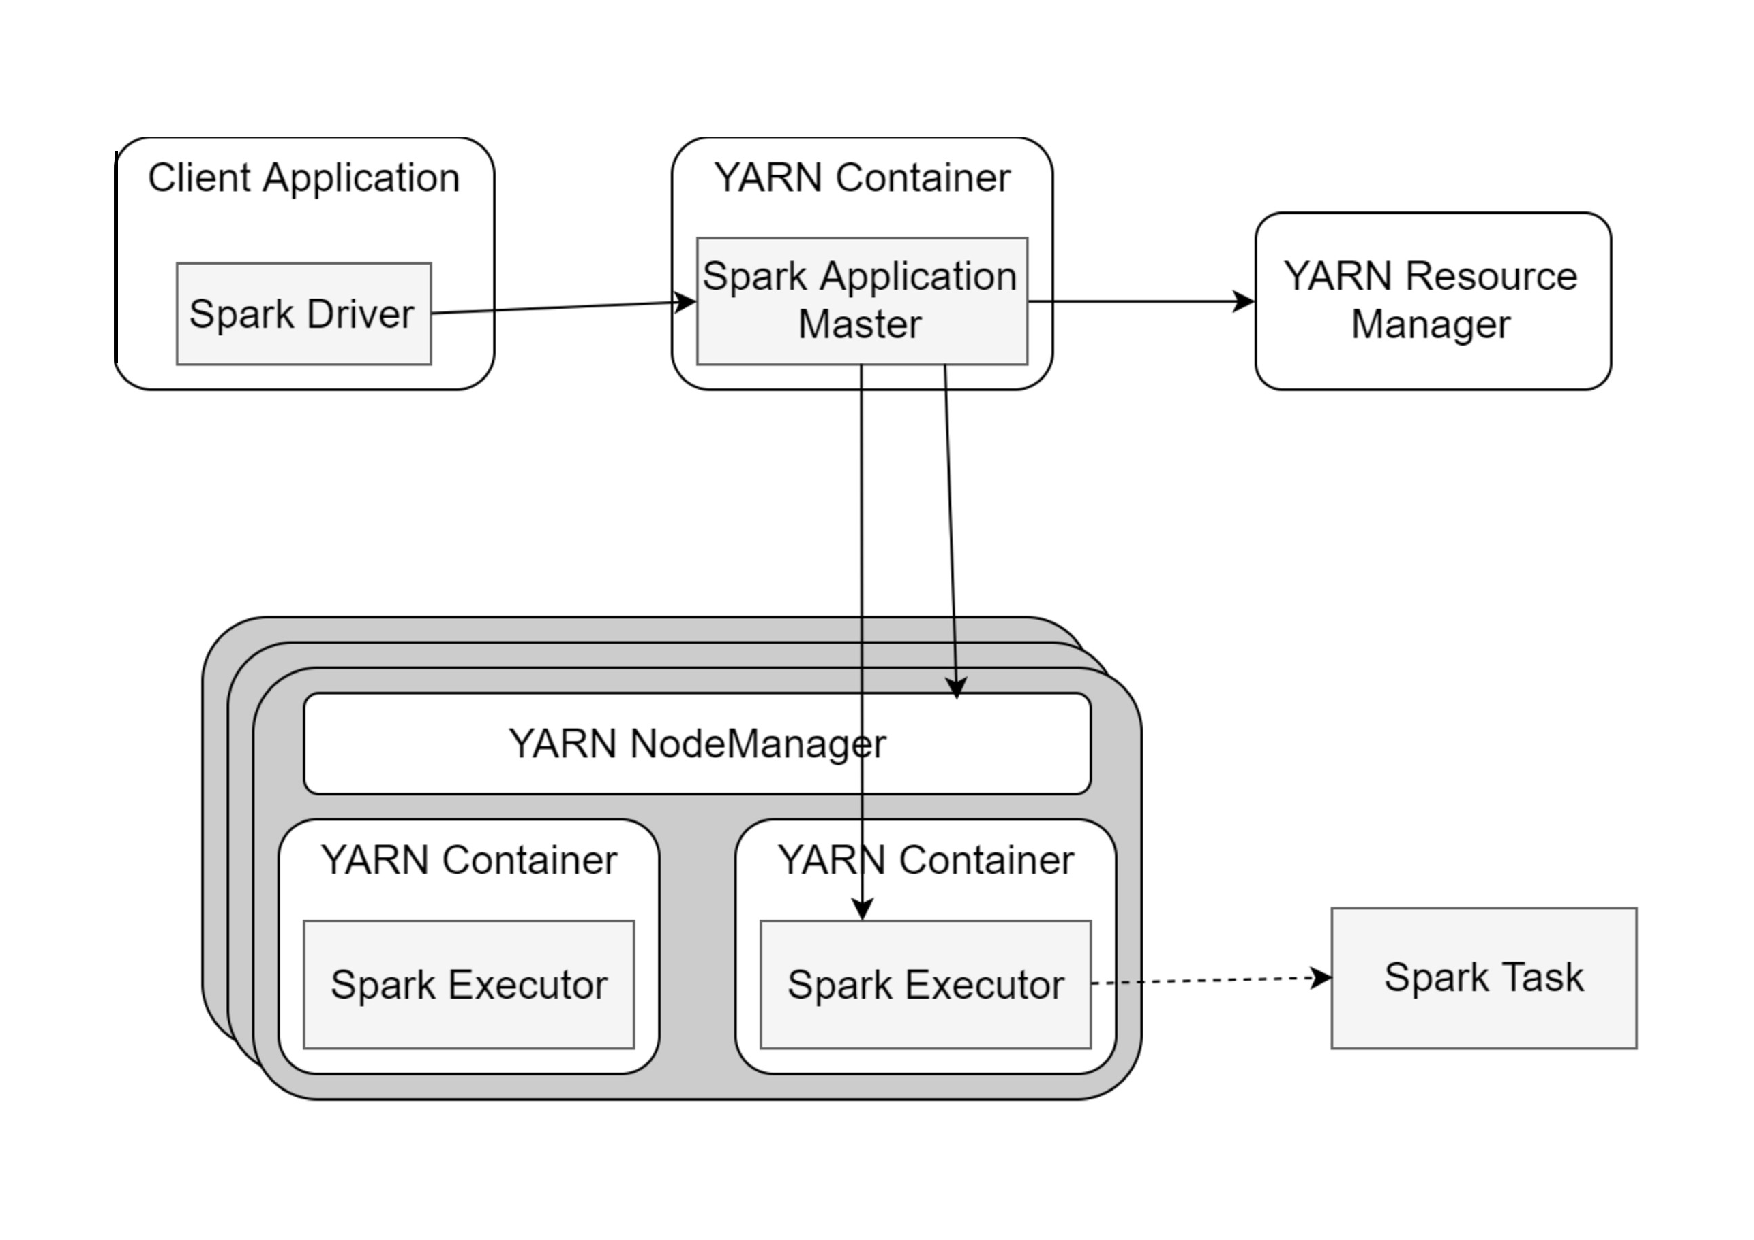
\includegraphics[width=\columnwidth]{Images/spark_yarn_client_mode.pdf}  
	\caption[Spark on YARN Client Mode]{Spark on YARN Client Mode.}
	\label{fig:sparkOnYarnClientMode}
\end{figure}
\begin{figure}
	\centering
	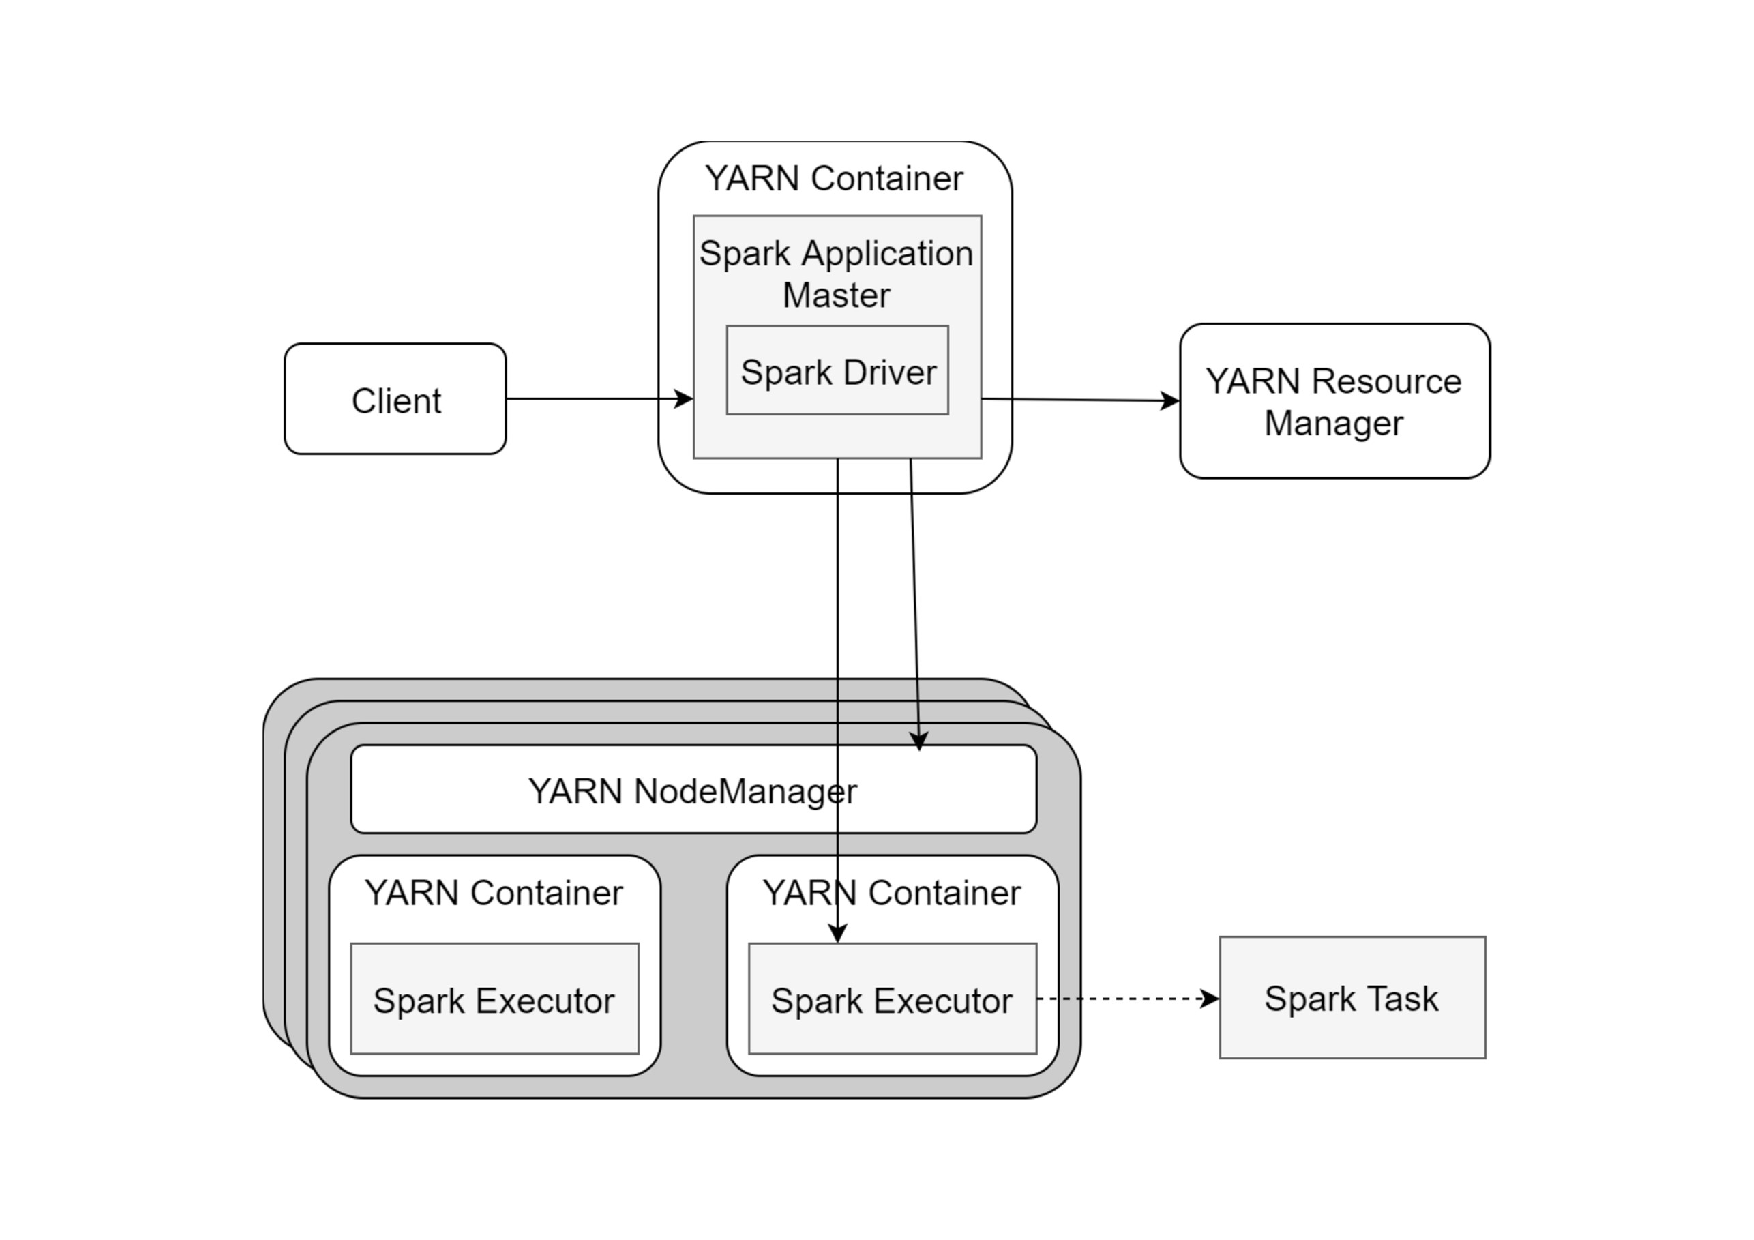
\includegraphics[width=\columnwidth]{Images/spark_yarn_cluster_mode.pdf}  
	\caption[Spark on YARN Cluster Mode]{Spark on YARN Cluster Mode.}
	\label{fig:sparkOnYarnClusterMode}
\end{figure}
\begin{figure}
	\centering
	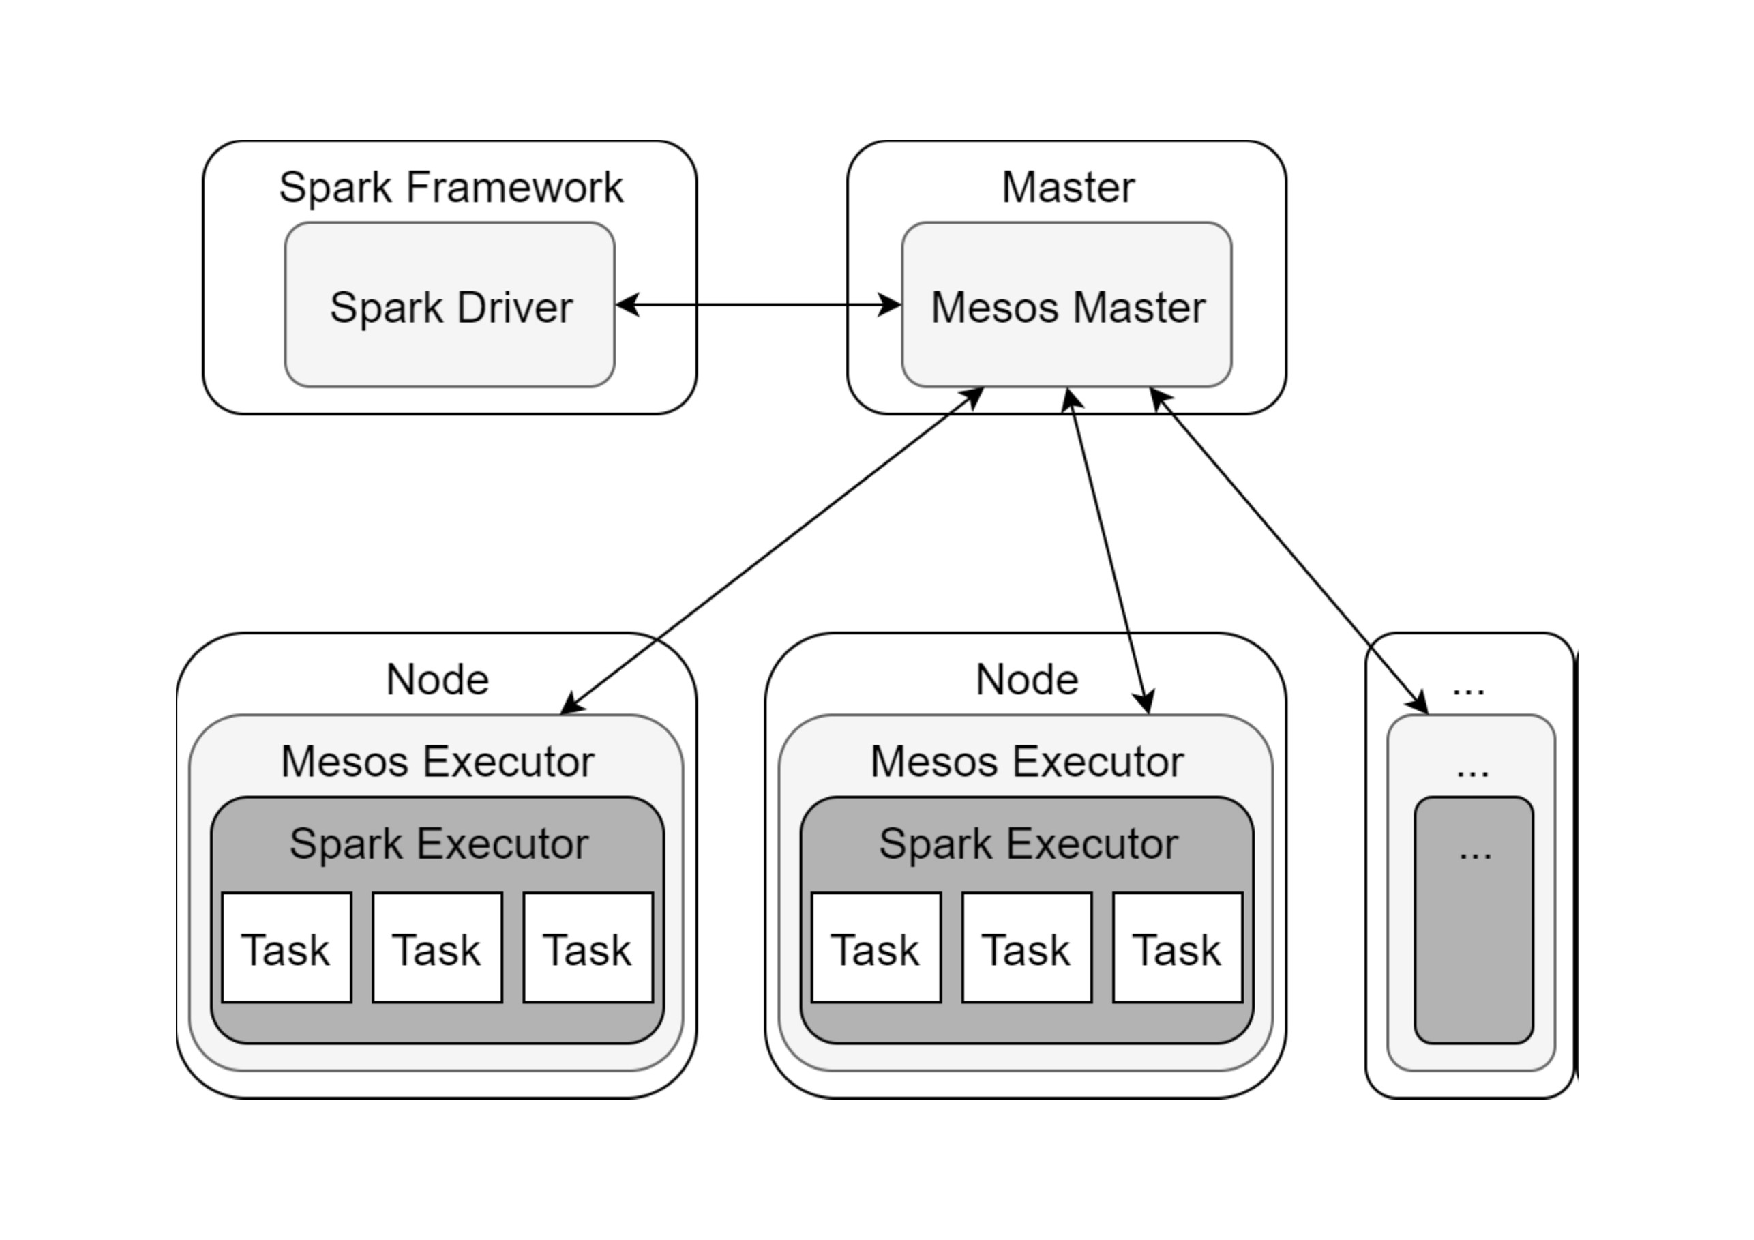
\includegraphics[width=\columnwidth]{Images/spark_mesos_coarse_grained_mode.pdf}  
	\caption[Spark on Mesos Coarse Grained Mode]{Spark on Mesos Coarse Grained Mode.}
	\label{fig:sparkOnMesosCoarseGrainedMode}
\end{figure}
\begin{figure}
	\centering
	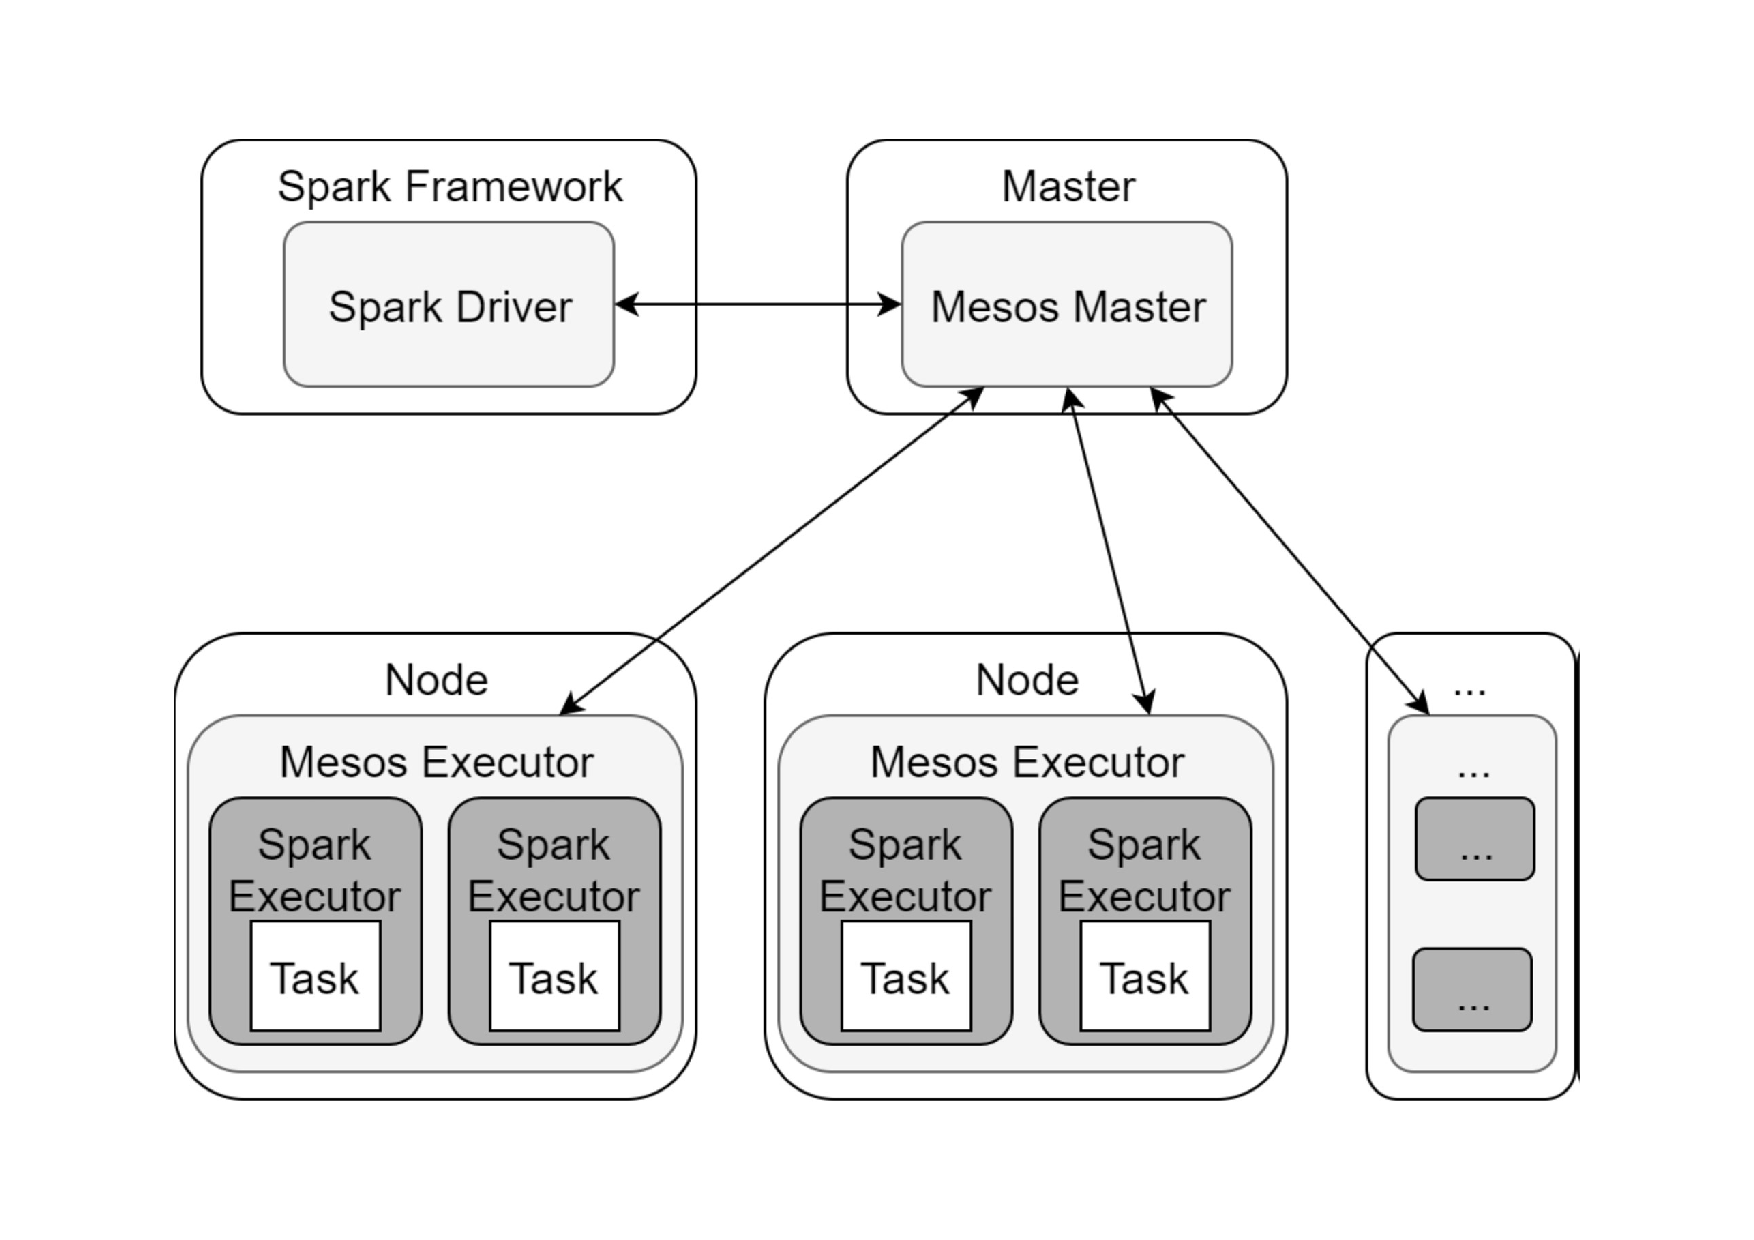
\includegraphics[width=\columnwidth]{Images/spark_mesos_fine_grained_mode.pdf}  
	\caption[Spark on Mesos Fine Grained Mode]{Spark on Mesos Fine Grained Mode.}
	\label{fig:sparkOnMesosFineGrainedMode}
\end{figure}

When running on YARN, Spark executors and driver program use
about 6-10\% more memory with respect to the standalone execution,
this is due to the fact that this extra amount of off-heap memory is
allocated in order to take into account YARN overheads.

\subsection{Spark on Mesos}{subsec:sparkOnMesos}
Support for running Spark on Mesos was added to Spark in version
1.5. Spark on Mesos can be executed in two different modes: coarse-grained
and fine-grained \cite{misc:SparkOnMesos}.
In coarse-grained mode, as shown in \myFig{fig:sparkOnMesosCoarseGrainedMode}, 
each Spark application is submitted to Mesos master as a framework and Mesos
slaves will run tasks for the Spark framework that are Spark executors.
Mesos tasks are launched for each Spark executor and those
Mesos tasks stay alive during the lifetime of the application unless
we are using dynamic allocation or the executor is killed for various
reasons. The advantage of coarse-grained mode is in a much lower task
startup overhead, with respect to the other mode, and so it is good
for interactive sessions.
The drawback is that we are reserving Mesos resources for the complete
duration of the application, unless dynamic allocation is active.
Dynamic allocation allows to add and remove executors based on
load: i) kill executor when they are idle, ii) add executors when tasks
queue up in the scheduler. To use dynamic allocation it is required
that the external shuffle service is running on each node.
In fine-grained mode, shown in \myFig{fig:sparkOnMesosFineGrainedMode}, 
Mesos tasks are launched for each Spark task, and those tasks die as soon as Spark tasks are done. This mode has too much overhead in case that Spark has too
many tasks, for example if Spark application has 10,000 tasks, then
Spark needs to be installed 10,000 times on Mesos agents. Because
of this huge overhead, fine-grained mode has been deprecated since
Spark version 2.0.0. This mode allows multiple instances of Spark to
share cores at a very fine granularity, but it comes with an additional
overhead in launching each task. Thus this mode is inappropriate
for low-latency requirements like interactive queries or serving web
requests, instead it is fine for batch and relatively static streaming.
Similarly to what happens on YARN, it is possible to run spark in
Mesos-client or Mesos-cluster mode. In client mode, the driver process
is executed in the client machine that submits the job, so it is required
that it stays connected to the cluster for the entire time of the application
execution. In cluster mode instead, the driver program is run on
a machine of the cluster.

\section{Virtualization and Containerization}
Virtualization refers to creating the virtual version of something, included
hardware components, storage devices and computer networks.
Virtualization is born in 1960's, as a way to logically partition the system
resources offered by a mainframe computer between many different
applications. From this point, the meaning of the word has been
widely extended.
Virtualization is a technology that allows creating multiple simulated
environments or dedicated resources from a single unique physical
hardware system. An hypervisor is a software that can directly
connect to the hardware, with the purpose of splitting the unique
physical system into separated environments, different from each other 
and secure, known as virtual machines (VM's). These VM's rely on
the hypervisor ability to separate the hardware resources and distribute
them in a proper way.
The original physical machine equipped with the hypervisor is
called host, meanwhile the VM's are called guests. These guests use the computation resources, such as CPU, memory and storage, as a set of resources that are easily re-allocatable. The operators can control the virtual instances of CPU, memory, storage
and other resources, so that the guests can receive all the resources they need
to execute their task. The words host and guest are used to distinguish the software that runs on the physical hardware from the software that is running on the virtual machines.
Hardware virtualization or platform virtualization refer to the creation
of a VM that acts like a real computer with an OS. The software
that is run in this VM is separated from the underlying hardware.
This allows us to run particular configurations, for example we run a
computer with a Windows OS that hosts a VM with Linux as guest OS.
There are at least two different hardware virtualization types:
\begin{itemize}
	\item full virtualization: it completely simulates the hardware in order
	to allow the software, typically a guest OS, to be run without the
	need of modifications
	\item paravirtualization: the hardware environment is not simulated,
	anyway guest programs are run in isolated domains, as if they
	were run in completely separated systems. Guest programs need
	to be modified in a specified way in order to run in this kind
	of environment.
\end{itemize}
\begin{figure}
	\centering
	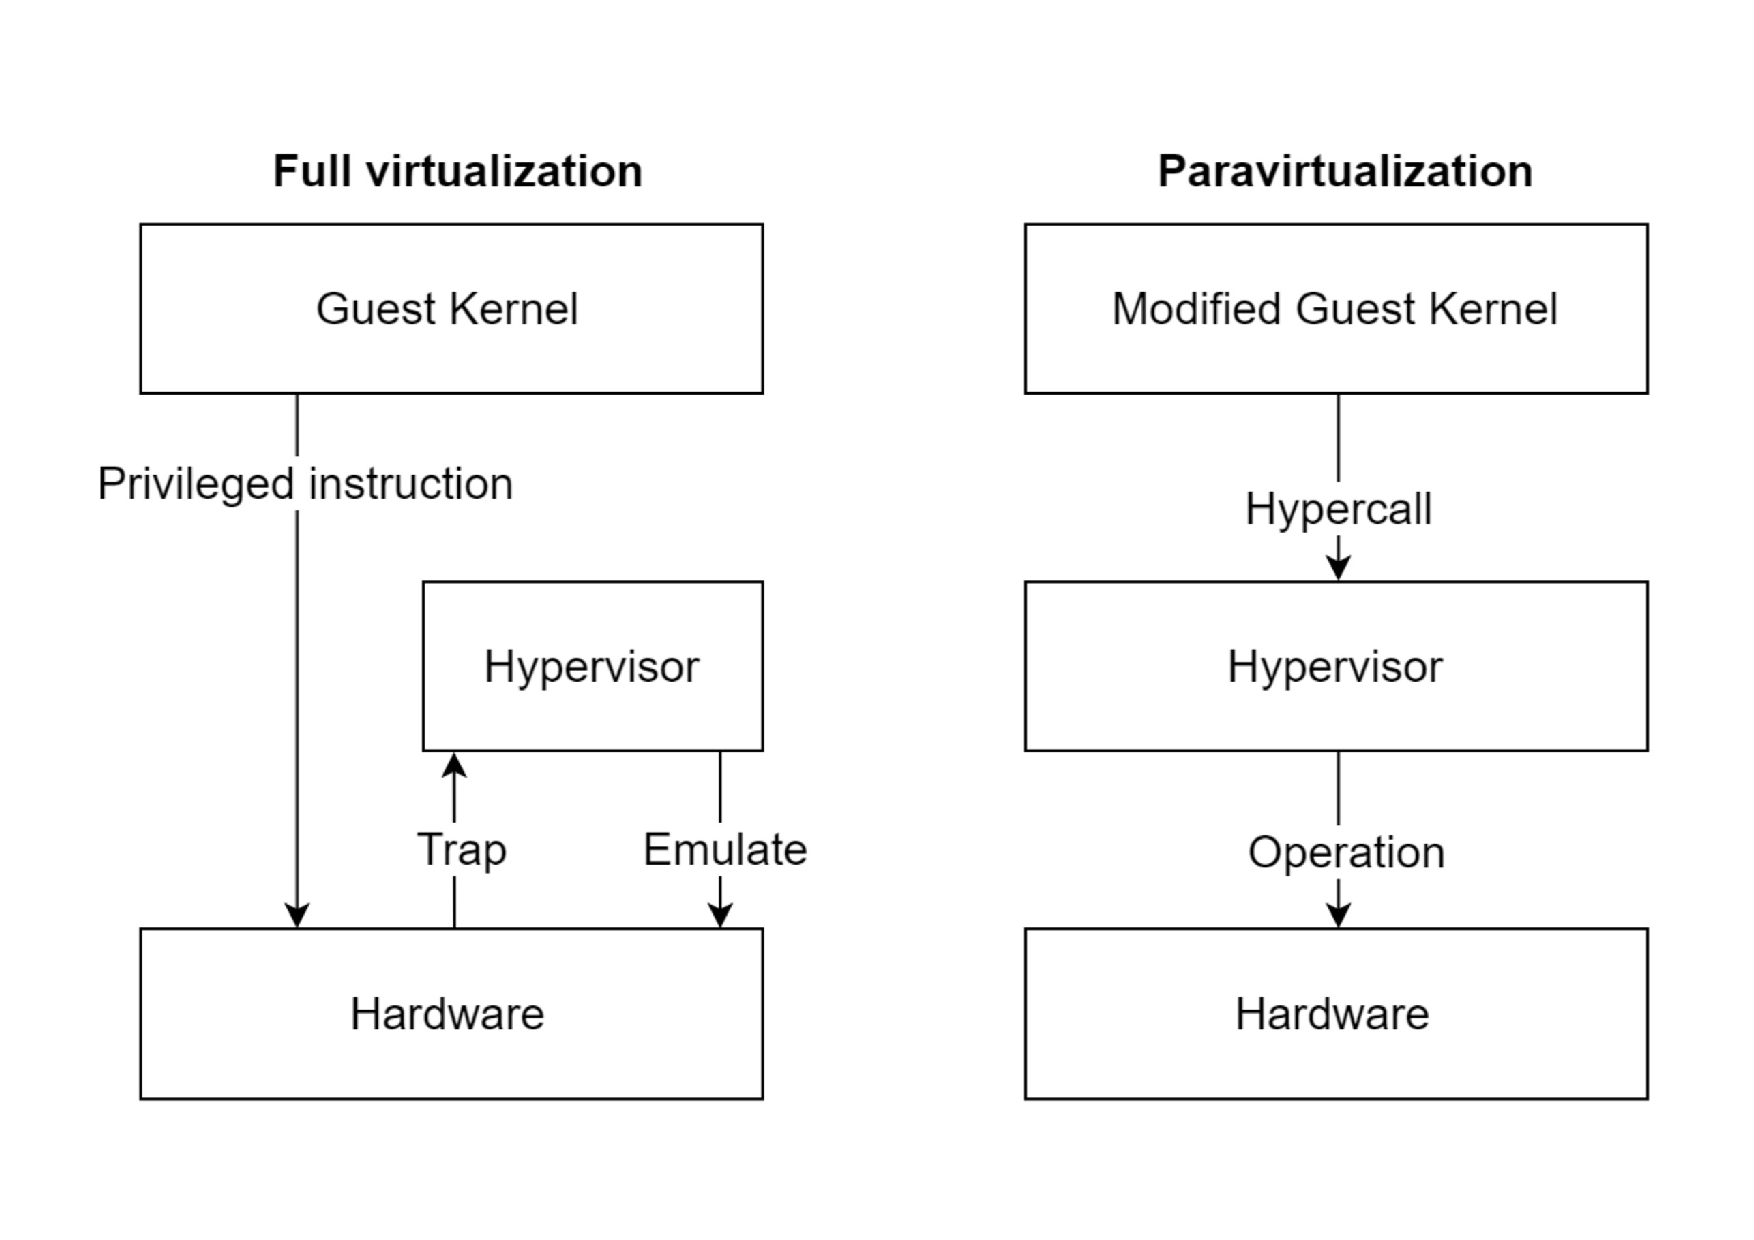
\includegraphics[width=\columnwidth]{Images/virtualization_paravirtualization.pdf}  
	\caption[Full virtualization and paravirtualization]{Full virtualization and paravirtualization.}
	\label{fig:virtualizationParavirtualization}
\end{figure}
In \myFig{fig:virtualizationParavirtualization}, we can see the differences between the two kind
of virtualization. In paravirtualization, the VM presents a different
interface compared to the one of a physical machine. This requires
modification in the guest OS in order to allow its execution inside
the VM. The hypervisor exposes a set of APIs that the guest OS must
use to execute privileged instructions. Calls to these particular functions are often defined as Hypercalls. In full virtualization instead, VM have the same interface as the physical ones. Ideally, the guest OS would not be able to determine if it is being
run on a physical or virtual machine. The great advantage of full
virtualization is that we do not need to modify the OS. In this way
the hypervisor can adopt a trap system to execute privileged
instructions. We can improve the efficiency of the virtualization by using hardware assisted virtualization, in particular we can decide to use CPU's that
provide efficient support for virtualizing on hardware, but also other
kind of hardware components that can improve the performance of
the guest environments.
Hardware virtualization can be seen as a trend of the enterprise IT
that includes autonomic computing, a scenario in which the different
environments are able to manage themselves based on the detected level of 
activity, and utility computing, where the processing power is seen
as a utility that users pay only when needed. The purpose of virtualization
is to centralize the administrative tasks, offering scalability and
good resource utilization. With virtualization, different OS can run
in parallel on a single CPU. This parallelism reduces overhead cost
in a way different from multitasking, where different
programs are executed in parallel on the same OS. 
Thanks to virtualization, an enterprise IT can better handle updates and rapid changes in OS and applications, with little impact on users. Virtualization allows organizations
to have better efficiency and availability of resources and
applications.
It is important to remember that hardware emulation is a complete
different thing from hardware virtualization, in particular with emulation
we have a piece of hardware that imitates another piece of
hardware. In virtualization instead a hypervisor, which is a piece
of software, mimics a piece of hardware or even an entire computer.
Moreover, a hypervisor is not an emulator, even though both are
software programs that mimic hardware, their domain of use is different.
\begin{figure}
	\centering
	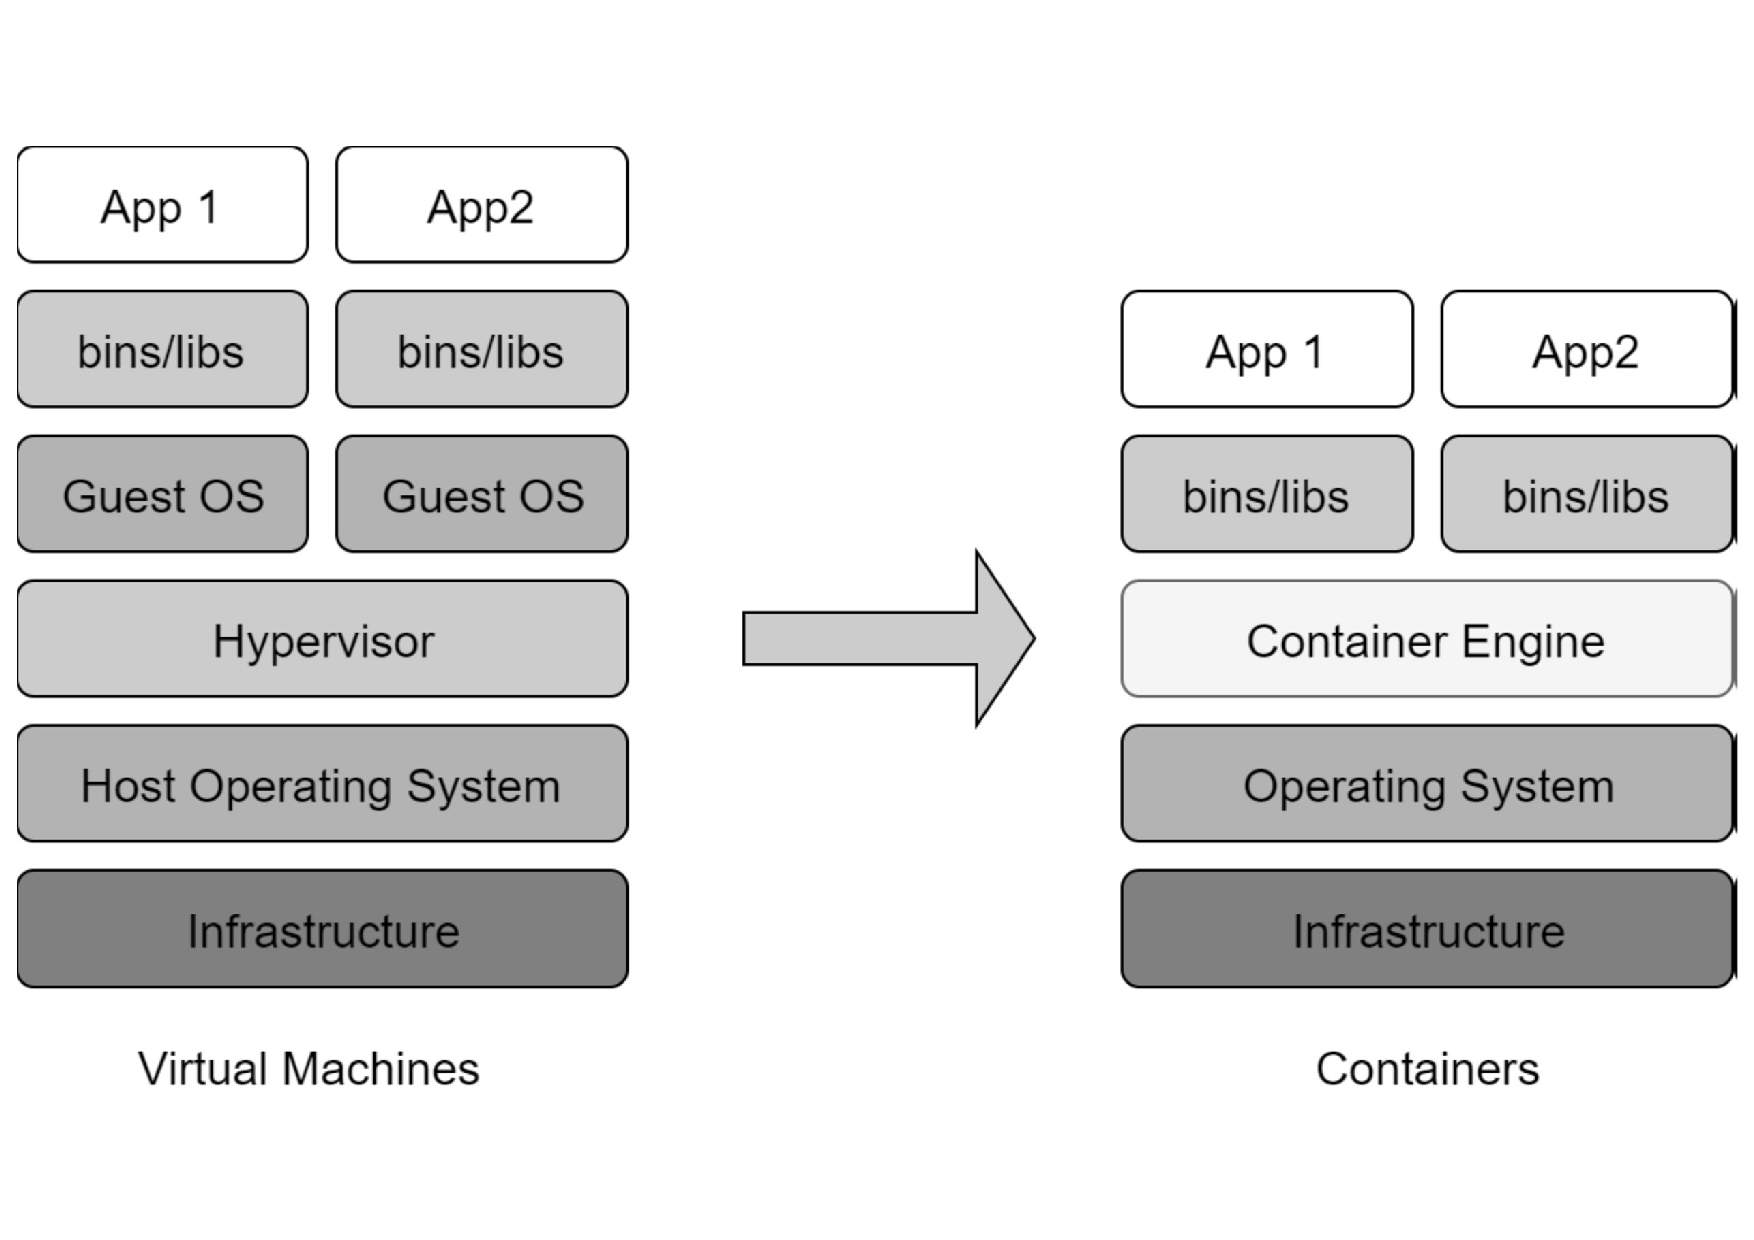
\includegraphics[width=\columnwidth]{Images/vm_vs_container.pdf}  
	\caption[Architecture of virtual machines and containers]{The difference in  architecture between virtual machines and containers.}
	\label{fig:vmVsContainer}
\end{figure}
Containerization is a OS-level virtualization technique that allows
deploying and executing distributed applications without the need
of launching an entire VM for each of the applications (\myFig{fig:vmVsContainer}).
These multiple isolated systems are called containers. They are executed
on top of a single host controller and access a single kernel.
Since containers share the same OS kernel of the host, they can be a lot
more efficient than a VM, that instead needs a separate instance of the
OS. Containers own all the different components that are needed in
order to execute the desired software, such as files, environment variables
and libraries. The host OS controls the access of the container to
the physical resources, such as CPU and memory, in order to prevent
a single container from occupying the entire resources offered by the
host.
The main advantages of containerization come from efficiency in
terms of memory, CPU and storage, when compared to traditional
hardware virtualization. Since containers do not have the same overhead
of VM, in particular we do not need different instances of the OS and 
is possible to support more containers on the same infrastructure.
Containerization offers better performances since there is a single OS
that takes care of all the hardware calls. A special advantage 
of the containers is the fact that they can be created much faster than
instances based on an hypervisor. This allows to have a more agile environment and allows the creation of new approaches to virtualization, such as microservices and continuous integration and delivery of services.
Potential disadvantages of containerization are the absence of
isolation from the host OS. Since containers share the same host OS, a
potential security threat might easily gain access to the entire system.
This does not happen when using virtualization based on a hypervisor,
since in this case the only compromised component would be the
VM. A way to circumvent this problem, is the creation of 
containers inside an OS run from a VM. This prevents the
security breach at container level from letting the attacker gain access
to the OS of the physical host. Another little disadvantage of containerization is that containers must execute the same OS as the base OS,
meanwhile instances based on an hypervisor are allowed to execute
different OSs. Because of this, a container that is running on a Linux
host, can neither execute an instance of Windows OS nor a Windows
designed application.
Containerization has gained more and more relevance thanks to
the wide spread of the open source software Docker, that has developed
aenhanced portability to the containers, allowing them to
be moved from different systems that share the same kind of host
OS without the need to change even a single line of code. In particular, with
Docker container there are no environment variables that must be set
on the guest OS or library dependencies that need to be managed.

%\subsection{Docker}{subsec:docker}
%Docker is an open source project that automatizes the deployment of applications inside software containers, giving a further abstraction thanks to OS level virtualization provided by Linux OS. Docker uses isolation functionalities provided by Linux kernel, such as cgroups and namespaces \cite{misc:Docker} in order to allow the coexistence of independent containers on the same Linux instance, avoiding the installation and maintenance of a VM. Linux kernel namespaces isolate what the application ca see of the operating environment, including process tree, network, user ids and mounted file system. Cgroups instead provide resource isolation, including CPU, memory, I/O devices and network.Docker implements a high level API in order to manage containers that execute in isolated environments. Since it uses Linux kernel functionalities, a Docker container, compared to a VM, does not includes a separated OS. Instead, it uses the kernel functionalities and exploits resource isolation and separated namespace in order to separate isolate what each application can see of the underlying OS. Docker can access Linux kernel virtualization functionalities using different ways, for example directly using libcontainer or indirectly using libvirt, Linux Containers (LXC) or systemd-nspawn (\myFig{fig:docker}). Using containers, resources can be isolated, services can be limited and processes can be started in a way that each of them has a private perspective of the OS, with their own identifier, file system and network interface. More container can share the same kernel, but each of them can be forced to use a different amount of resources such as CPU, memory and I/O. By using Docker we can create and manage container in a way that simplifies the creation of distributed systems, allowing different applications and processes to work in an autonomous way on the same physical machine or on different virtual machines. This allows us to deploy new nodes only when necessary, in order to follow an evolution style that is similar to the platform as a service one.
%\begin{figure}
%	\centering
%	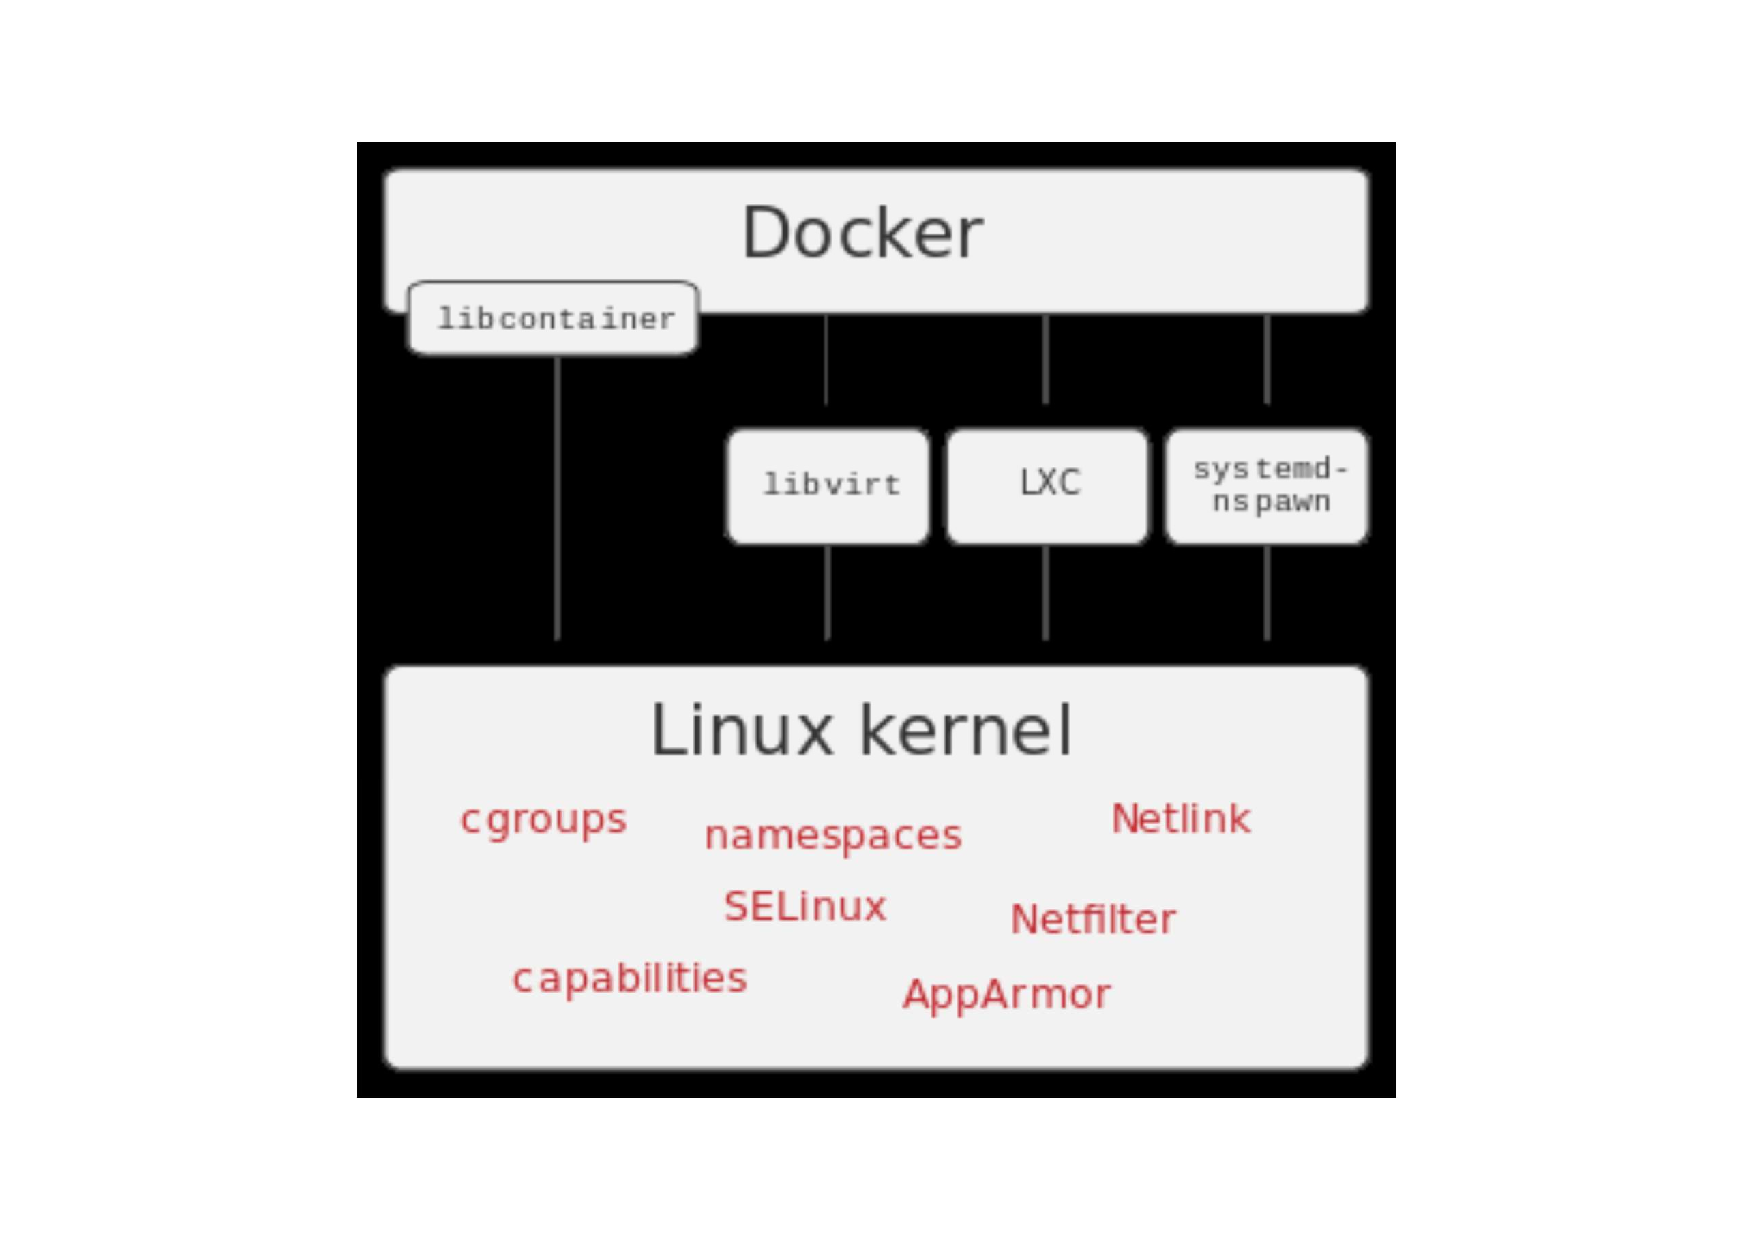
\includegraphics[width=\columnwidth]{Images/docker.pdf}  
%	\caption[Docker Interfaces]{Docker can use different interfaces in order to access Linux %kernel virtualization functionalities.}
%	\label{fig:docker}
%\end{figure}

\section{Symbolic Execution}
In computer science, the term symbolic execution refers to a software program analysis technique used to determine which data inputs cause These execution of each part of a program. It was introduced in the mid '70s~\cite{K-ICRS75,SELECT-ICRS75,K-CACM76,H-TSE77} mainly to test whether a software program could violate certain properties, e.g. that no divisions by zero are performed, no NULL pointers get dereferenced, no access to protected data can happen by unathorized users, etc. In general, it's not possible to decide every possible program property by means of automated checks, for example we cannot predict the target of an indirect jump. %, as it depends on values that are known at runtime. 
In practice, approximate and heuristic-based analyses are used in many cases, even in the field of mission-critical and security applications.

Software testing is performed to check that certain program properties hold for any possible usage scenario. A viable approach would be to test the program using a wide range of different, possibly random inputs. As the problem may occur only for very specific input values, we need to automate the exploration of the domain of the possible input data. 

With symbolic execution many possible execution paths are explored in parallel, without necessarily requiring concrete inputs. The idea is to replace the fully specified input data with symbols, that are their abstract representation, devolving to constraint solvers the construction of actual instances that would cause property violations. 

The symbolic execution intepreter walks through all the steps of the program, associating symbolic values to inputs rather than obtaining their actual values, building  expressions in terms of those symbols and program variables, and constraints in terms of the symbols corresponding to the possible outcomes of each conditional branch. 

When a program is run with a specific set of input data (a concrete execution), a single control flow path is explored. Hence, concrete executions can only under-approximate the analysis of the property of interest. With symbolic execution, multiple paths that a program could take under different inputs can be simultaneously explored. This means that a sound analyses can be done, giving stronger guarantees about the checked property~\cite{Baldoni:2018:SSE:3212709.3182657}. When a program runs with {\em symbolic} -- rather than concrete -- input values, the execution is performed by a {\em symbolic execution engine}, which builds and updates a structure to hold (i) a first-order Boolean {\em formula} describing the conditions satisfied by all the traversed branches along that path, and (ii) a {\em symbolic memory store} mapping variables to symbolic expressions or values, for each path traversed by the control flow. Execution of a branch updates the formula, while assignments update the symbolic store. Finally, a {\em model checker}, commonly based on a {\em satisfiability modulo theories} (SMT) solver~\cite{BKM14}, is  used to verify if the property is violated somewhere along each explored path and if the path itself is concretely feasible, i.e., if any assignment of concrete values to the program's symbolic arguments exists that satisfies its formula~\cite{Baldoni:2018:SSE:3212709.3182657}.

Symbolic execution techniques have been emphasized to a wide audience following the DARPA announcement in 2013 at the Cyber Grand Challenge, a two-year competition pursuing the creation of automatic systems for vulnerability detection, exploitation, and patching in near real-time~\cite{ANGR-SSP16}.
More important, symbolic execution based engines have been running 24/7 in the testing process of many Microsoft applications since 2008, discovering nearly 30\% of all the flaws discovered by file fuzz testing during the development of Windows 7, which other program analyses and blackbox testing techniques missed~\cite{SAGE-QUEUE12}.

\paragraph{An Introductory Example}


\label{symbolic-execution-example}
\begin{figure}[t]
	\begin{center}
		\begin{tabular}{c}
			\begin{lstlisting}[basicstyle=\ttfamily\scriptsize]
			1.  void foo(int a, int b) {
			2.     int x = 1, y = 0;
			3.     if (a != 0) {
			4.        y = 3+x;
			5.        if (b == 0)
			6.           x = 2*(a+b);
			7.     }
			8.     assert(x-y != 0);
			9.  }
			\end{lstlisting}
		\end{tabular}
	\end{center}
	\vspace{-2mm}
	\caption{Example: which values of \texttt{a} and \texttt{b} make the \texttt{assert} fail?}
	\label{fig:example-1}
	\vspace{-1.5mm}
\end{figure}

With reference to the C code in \MyFig{fig:example-1}, let's say we want to discover which of the $2^{32}$ possible \texttt{4-byte} inputs make the \texttt{assert} at line 8 of function \texttt{foo} fail. If we address the problem by running concretely the function \texttt{foo} on randomly generated inputs, we will unlikely pick up exactly the assert-failing inputs. Symbolic execution go beyond this limitation by reasoning on {\em classes of inputs}, rather than single input values, thanks to the evaluation of the code using symbols for its inputs, instead of concrete values,  

Going further into details, a symbol $\alpha_i$ is associated to each value that cannot be resolved by a static analysis of the code, e.g. an actual parameter of a function or data read from an input stream. At any time, the symbolic execution engine maintains a state $(stmt,~\sigma,~\pi)$ where:

\begin{itemize}
	\item $stmt$ is the next statement to evaluate. At this time being, we assume that $stmt$ can be an assignment, a conditional branch, or a jump.
	
	\item $\sigma$ is a {\em symbolic store} that associates program variables with either expressions over concrete values or symbolic values $\alpha_i$.
	
	\item $\pi$ denotes the {\em path constraints}, i.e., it is a formula expressing a set of assumptions on the symbols $\alpha_i$ as a result of branches taken in the execution to reach $stmt$. At the start of the analysis, $\pi=true$.
\end{itemize}

\noindent Depending on $stmt$, the symbolic engine changes the state as follows:

\begin{itemize}
	\item The evaluation of an assignment $x=e$ updates the symbolic store $\sigma$ by associating $x$ with a new symbolic expression $e_s$. We express this association with $x\mapsto e_s$, where $e_s$ is obtained by evaluating $e$ in the context of the current execution state and  can be any expression involving unary or binary operators over symbols and concrete values.
	\item The evaluation of a conditional branch ${\texttt if}~e~{\texttt then}~s_{true}~{\texttt else}~s_{false}$ affects the path constraints $\pi$. The symbolic execution is forked by creating two execution states with path constraints $\pi_{true}$ and $\pi_{false}$, respectively, which correspond to the two branches: $\pi_{true}=\pi \wedge e_s$ and $\pi_{false}=\pi \wedge \neg e_s$, where $e_s$ is a symbolic expression obtained by evaluating $e$. 
	Symbolic execution independently proceeds on both states.
	\item The evaluation of a jump {\texttt goto} $s$ updates the execution state by advancing the symbolic execution to statement $s$. 
\end{itemize}

\begin{figure}[t]
	\centering
	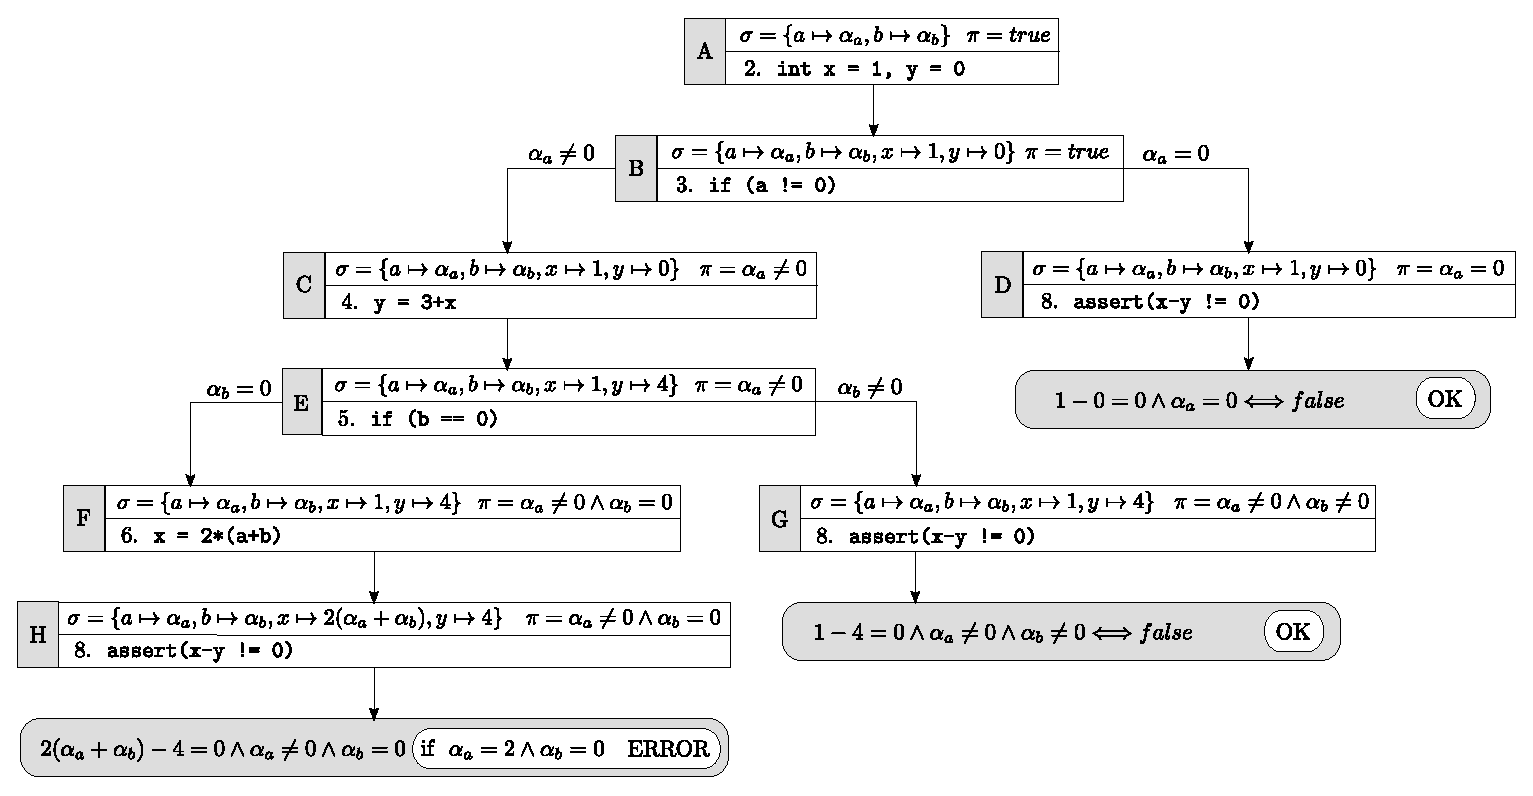
\includegraphics[width=0.975\columnwidth]{images/execution-tree.eps} 
	\caption{Symbolic execution tree of function {\texttt foo} given in \MyFig{fig:example-1}. Each execution state, labeled with an upper case letter, shows the statement to be executed, the symbolic store $\sigma$, and the path constraints $\pi$. Leaves are evaluated against the condition in the {\texttt assert} statement. }
	%For the sake of presentation the conjunction of constraints is shown as a list of constraints. }
	\label{fig:example-symbolic-execution}
	\vspace{-1mm}
\end{figure}

\noindent \MyFig{fig:example-symbolic-execution} shows a symbolic execution of function {\texttt foo}, that can be adequately represented as a tree. In the initial state (execution state $A$) the path constraints are {\texttt true} and input arguments {\texttt a} and {\texttt b} are associated with symbolic values. 
After local variables initialization {\texttt x} and {\texttt y} at line 2, the symbolic store is updated by associating {\texttt x} and {\texttt y} with concrete values 1 and 0, respectively (execution state $B$). A conditional branch is met in line 3 and the execution is forked:according to which branch is taken, a different statement is evaluated and different assumptions are made on symbol $\alpha_a$ (execution states $C$ and $D$). In the branch corresponding to $\alpha_a\neq 0$, variable {\texttt y} is assigned to  ${\texttt x}+3$, obtaining $y\mapsto 4$ in state $E$ because $x\mapsto 1$ in state $C$. Arithmetic expression evaluation, generally, change only the symbolic values.
When the {\texttt assert} at line 8 is reached by fully expanding every execution state  on all branches, we can check which input values for parameters {\texttt a} and {\texttt b} can make the {\texttt assert} fail. By analyzing execution states $\{D,G,H\}$, we can conclude that only $H$ can make {\texttt x-y = 0} true. The path constraints for $H$ at this point implicitly define the set of inputs that are unsafe for \texttt{foo}. 
In particular, any input values such that:
\[ 2(\alpha_a+\alpha_b)-4 = 0 \wedge \alpha_a \neq 0 \wedge \alpha_b = 0 \]
will make {\texttt assert} fail. An instance of unsafe input parameters can be eventually determined by invoking an {\em SMT solver}~\cite{BKM14} to solve the path constraints, which in this example would yield $a = 2$ and $b = 0$.

\subsubsection{Challenges of Symbolic Execution}
\label{example-discussion}

The example shown in Section~\ref{symbolic-execution-example} represents a case where symbolic execution can derive {\em all} the inputs that make the {\texttt assert} fail, by exploring all the possible execution states. With regards to the underpinning theory, exhaustive symbolic execution represents a {\em sound} and {\em complete} methodology for any decidable analysis. Soundness (no false negatives) means that all possible unsafe inputs are guaranteed to be found, while completeness (no false positives) means that  input values deemed unsafe are actually unsafe. Exhaustive symbolic execution cannot be easily scalable beyond small-sized applications. In many practical cases, a trade-off between soundness and performance approach is used.

Symbolic execution applied to real world applications faces many challenges, deriving from the increased complexity of those applications compared to the simplicity of our example. These challenges are pointed out by the following questions and observations:

\begin{itemize}
	\item \noindent {\em Pointers, arrays, or other complex objects}: how are they handled by the symbolic engine? Code manipulating pointers and data structures may identify memory addresses that are described by symbolic expressions, in addition to symbolic stored data.
	\item {\em Interactions across the software stack}: how are they handled by the engine? System code/library calls can have side effects, e.g. file creations, calls back to user code or callback functions that could affect the execution at a later stage of the computation and must be taken in account. 
	Evaluating all possible interaction outcomes may be unfeasible.
	\item {\em State space explosion}: how does symbolic execution deal with path explosion? The presence of iterative constructs in the language (iteration loops) can dramatically increase the number of execution states, up to the point where it becomes unfeasible for a symbolic execution engine to exhaustively explore all the possible states within a reasonable amount of time. 
	\item {\em Constraint solving}: what can a constraint solver do in practice?
	SMT solvers can scale to complex combinations of constraints over hundreds of variables. However, constructs such as non-linear arithmetic pose a major obstacle to efficiency.
	\item {\em Binary code}: what issues can arise when symbolically executing binary code?
	While our example of Section~\ref{symbolic-execution-example} is written in C, in many cases programs are only available as binary code. The availability of the source code of an application usually simplifies symbolic execution, as it can exploit high-level properties (e.g., object morphology) that can be inferred statically by analyzing the source code.
\end{itemize}
%Depending on the specific application context of symbolic execution

\noindent The above questions and assumptions are addressed in different ways and lead to different choices according to the specific contexts where symbolic execution is used. Typically these choices affect soundness or completeness, however this does not represent a serious limitation in many real cases where a partial exploration of the domain of possible execution states may provide enough information to reach the goal (e.g., determining which input values provokes an application failure) within specified time limits.

\subsection{Symbolic Execution Engines}
\label{se:executors}

In this section we describe some important ementation. Moving from the concepts of concrete and symbolic runs, we also introduce the idea ofprinciples for the design of symbolic executors and crucial tradeoffs that arise in their impl {\em concolic} execution.

\subsubsection{Mixing Symbolic and Concrete Execution}
\label{ss:concrete-concolic-symbolic}

\begin{figure}[t]
	\centering
	%\vspace{-0.75mm}
	
\includegraphics[width=0.32\columnwidth]{images/concrete-abstract.eps} 
	\caption{Concrete and abstract execution machine models.}
	\label{fig:concrete-symbolic}
	\vspace{-1.5mm}
\end{figure}

As shown in the previous example, modeling all runs of concrete executions of real-world software programs is desirable but very often impossible in practice.

Symbolic execution, as we have described it so far, cannot explore feasible executions that would result in path constraints that cannot be dealt with~\cite{CS-CACM13}. Loss of soundness originates from many sources, e.g. untraceable external code, complex constraints involving non-linear arithmetic or transcendental functions. As constraint solving is a major performance barrier for an engine, we can assess the solvability in an absolute sense but also in terms of efficiency. Considering that practical programs are typically not self-contained, it is very challenging to statically analyze the whole software stack, especially considering the evaluation of every possible side effects.

One way to overcome this issue in practice is to mix concrete and symbolic execution, aka {\em concolic execution}, where the term concolic is a portmanteau of the words ``concrete'' and ``symbolic'' (Figure~\ref{fig:concrete-symbolic}). Some applications of this general principle are briefly discussed in the remainder of this section.


\newcommand{\dse}{DSE}
\paragraph{Dynamic Symbolic Execution} A common approach to concolic execution, known as {\em dynamic symbolic execution} (\dse) or {\em dynamic test  generation}~\cite{DART-PLDI05}, is to have concrete execution drive the symbolic one. A concrete store $\sigma_c$ is maintained, in addition to the symbolic and the path constraints stores, by the execution engine. It chooses an initial arbitrary input and executes the program both concretely and symbolically, by simultaneously updating the two stores and the path constraints. The symbolic execution wlaks through the same branch taken by the concrete execution, and the constraints extracted from the branch condition are added to the current set of path constraints. The symbolic engine does not need to invoke the constraint solver to decide if a branch condition is satisfiable, as this is already tested by the concrete execution. Since not all the paths might be explored by concrete execution, the path conditions associated to a branch can be negated and passed to the SMT solver to determine a satisfying assignment for the new constraints, i.e., to generate a new input. This strategy can be repeated until the desired path coverage is reached.

\vspace{-2pt} 
%\boxedexample{
\fbox{
\begin{minipage}{4.3 in}
	Consider the C function in Figure~\ref{fig:example-1} and suppose to choose $a = 1$ and $b = 1$ as input parameters. Under these conditions, the concrete execution takes path $A\leadsto B\leadsto C\leadsto E\leadsto G$ in the symbolic tree of Figure~\ref{fig:example-symbolic-execution}. Besides the symbolic stores shown in Figure~\ref{fig:example-symbolic-execution}, the concrete stores maintained in the traversed states are the following:
	\begin{enumerate}
		
		\item[]$-$~~$\sigma_c=\{a\mapsto 1,~b\mapsto 1\}$ in state $A$;
		\item[]$-$~~$\sigma_c=\{a\mapsto 1,~b\mapsto 1,~x\mapsto 1,~y\mapsto 0\}$ in states $B$ and $C$;
		\item[]$-$~~$\sigma_c=\{a\mapsto 1,~b\mapsto 1,~x\mapsto 1,~y\mapsto 4\}$ in states $E$ and $G$.
		
	\end{enumerate}  
	%Stores and path constraints maintained by the concolic run are shown in Figure~\ref{fig:example-concolic-execution}. 
	After checking that the \texttt{assert} conditions at line 8 succeed, we can generate a new control flow path by negating the last path constraint, i.e., $\alpha_b\neq 0$. The solver at this point would generate a new input that satisfies the constraints $\alpha_a\neq 0\,\wedge\, \alpha_b=0$ (for instance $a = 1$ and $b = 0$) and the execution would continue in a similar way along the path $A\leadsto B\leadsto C\leadsto E\leadsto F$. %
\end{minipage}}

\vspace{+10pt}
Although \dse\ uses concrete inputs to drive the symbolic execution toward a specific path, it still needs to pick a branch to negate whenever a new path has to be explored. Notice also that each concrete execution may add new branches that will have to be visited. Since the set of non-taken branches across all performed concrete executions can be very large, adopting effective search heuristics (Section~\ref{ss:heuristics}) can play a crucial role. For instance, {\textsc DART}~\cite{DART-PLDI05} chooses the next branch to negate using a depth-first strategy. Additional strategies for picking the next branch to negate have been presented in literature. For instance, the {\em generational search} of {\textsc SAGE}~\cite{SAGE-NDSS08} systematically yet partially explores the state space, maximizing the number of new tests generated while also avoiding redundancies in the search. This is achieved by negating constraints following a specific order and by limiting the backtracking of the search algorithm. Since the state space is only partially explored, the initial input plays a crucial role in the effectiveness of the overall approach.  The importance of the first input is similar to what happens in traditional {\em black-box fuzzing}; hence, symbolic engines such as {\textsc SAGE} are often referred to as {\em white-box fuzzers}.

The symbolic information maintained during a concrete run can be exploited by the engine to obtain new inputs and explore new paths. The next example shows how DSE can handle invocations to external code that is not symbolically tracked by the concolic engine.



\vspace{10pt}
%\boxedexample{
\fbox{
	\begin{minipage}{4.3 in}
	Consider function {\texttt foo} in Figure~\ref{fig:example-concolic-problems}a and suppose that {\texttt bar} is not symbolically tracked by the concolic engine (e.g., it could be provided by a third-party component, written in a different language, or analyzed following a black-box approach). Assuming that $x = 1$ and $y = 2$ are randomly chosen as the initial input parameters, the concolic engine executes {\texttt bar} (which returns $a = 0$) and skips the branch that would trigger the error statement. At the same time, the symbolic execution tracks the path constraint $\alpha_y \geq 0$ inside function {\texttt foo}. Notice that branch conditions in function {\texttt bar} are not known to the engine. To explore the alternative path, the engine negates the path constraint of the branch in {\texttt foo}, generating inputs, such as $x = 1$ and $y = -4$, that actually drive the concrete execution to the alternative path. With this approach, the engine can explore both paths in {\texttt foo} even if {\texttt bar} is not symbolically tracked. 
	
	A variant of the previous code is shown in Figure~\ref{fig:example-concolic-problems}b, where function {\texttt qux} -- differently from {\texttt foo} -- takes a single input parameter but checks the result of {\texttt bar} in the branch condition. Although the engine can track the path constraint in the branch condition tested inside {\texttt qux}, there is no guarantee that an input able to drive the execution toward the alternative path is generated: the relationship between $a$ and $x$ is not known to the concolic engine, as {\texttt bar} is not symbolically tracked. In this case, the engine could re-run the code using a different random input, but in the end it could fail to explore one interesting path in {\texttt qux}. 
	
	A related issue is presented by Figure~\ref{fig:example-concolic-problems}c. We observe a {\em path divergence} when inputs generated for a predicted path lead execution to a different path. In general, this can be due to symbol propagation not being tracked, resulting in inaccurate path constraints, or to imprecision in modeling certain (e.g., bitwise, floating-point) operations in the engine. In the example, function {\texttt baz} invokes the external function {\texttt abs}, which performs a side effect on $x$ by assigning it with its absolute value. Choosing $x = 1$ as the initial concrete value, the concrete execution does not trigger the error statement, but the concolic engine tracks the path constraint $\alpha_x \geq 0$ due to the branch in {\texttt baz}, trying to generate a new input by negating it. However the new input, e.g., $x = -1$, does not trigger the error statement due to the (untracked) side effects of {\texttt abs}. Interestingly, the engine has no way of detecting that no input can actually trigger the error.
	% {\texttt abs}, which simply computes the absolute value of a number
	%In this case, after generating a new input the engine detects a {\em path divergence}: a concrete execution that does not follow the predicted path. Interestingly, in this example no input could actually trigger the error, but the engine is not able to detect this property.
\end{minipage}}

\begin{figure*}[t]
	\vspace{-2.5mm}
	%\centering
	\begin{minipage}{.30\textwidth}
		\begin{lstlisting}[basicstyle=\ttfamily\scriptsize]
void foo(int x, int y) {
int a = bar(x);
if (y < 0) ERROR;
} 
		\end{lstlisting}
		%int bar(int z) {
		%   if (z == 23) return 1;
		%   return 0;
		%}
		\vspace{-4mm}
		%\caption{}
	\end{minipage}%
	%
	\hspace{5mm}
	%
	\begin{minipage}{.30\textwidth}
		%\vspace{5mm}
		\begin{lstlisting}[basicstyle=\ttfamily\scriptsize]
void qux(int x) {
int a = bar(x);
if (a > 0) ERROR;
} 
		\end{lstlisting}
		%int bar(int z) {
		%   if (z == 23) return 1;
		%   return 0;
		%}
		\vspace{-4mm}
		%\caption{}
	\end{minipage}%
	%
	\hspace{5mm}
	%
	\begin{minipage}{.30\textwidth}
		%\vspace{5mm}
		\begin{lstlisting}[basicstyle=\ttfamily\scriptsize]
void baz(int x) {
abs(&x);
if (x < 0) ERROR;
}   
		\end{lstlisting}
		%void abs(int * z) {
		%   if (*z < 0) *z = -(*z);
		%}
		\vspace{-4mm}
		%\caption{}
	\end{minipage}%
\begin{Verbatim}[obeytabs]
	a)		     b)			c)
\end{Verbatim}
	\vspace{+2pt}
	\caption{Concolic execution: (a) testing of function {\texttt foo} even when {\texttt bar} cannot be symbolically tracked by an engine, (b) example of false negative, and (c) example of a path divergence, where \texttt{abs} drops the sign of the integer at \texttt{\&x}.
		%(b) Example of a missed path: assuming that function {\tt bar} is not symbolically tracked, then it is unlikely that the engine will be able to generate an input that trigger execution of function {\tt error} inside function {\tt qux}. (c) Example of a path divergence: assuming that function {\tt abs} is not tracked, then the concolic engine may try to generate fruitlessly an input able to trigger execution of function {\tt error} in function {\tt baz}.
	}
	\label{fig:example-concolic-problems}
	\vspace{-3mm}
\end{figure*}




As shown by the example, false negatives (i.e., missed paths) and path divergences are notable downsides of dynamic symbolic execution. \dse\ trades soundness for performance and implementation effort: false negatives are possible, because some program executions -- and therefore possible erroneous behaviors -- may be missed, leading to a {\em complete}, but {\em under-approximate} form of program analysis. Path divergences have been frequently observed in literature: for instance,~\cite{SAGE-NDSS08} reports rates over $60\%$. \cite{CLH-SCN15} presents an empirical study of path divergences, analyzing the main patterns that contribute to this phenomenon. External calls, exceptions, type casts, and symbolic pointers are pinpointed as critical aspects of concolic execution that must be carefully handled by an engine to reduce the number of path divergences.

\paragraph{Selective Symbolic Execution}
{\textsc \stwoe}~\cite{CKC-TOCS12} takes a different approach to mix symbolic and concrete execution based on the observation that one might want to explore only some components of a software stack in full, not caring about others. {\em Selective symbolic execution} carefully interleaves concrete and symbolic execution, while keeping the overall exploration meaningful.
%{\em Selective symbolic execution} carefully interleaves concrete executions of functions with fully symbolic phases, while keeping the exploration meaningful.

Suppose a function A calls a function B and the execution mode changes at the call site. Two scenarios arise:
(1) {\em From concrete to symbolic and back}: the arguments of B are made symbolic and B is explored symbolically in full. B is also executed concretely and its concrete result is returned to A. After that, A resumes concretely. 
(2) {\em From symbolic to concrete and back}: the arguments of B are concretized, B is executed concretely, and execution resumes symbolically in A. This may impact both soundness and completeness of the analysis: (i) {\em Completeness}: to make sure that symbolic execution skips any paths that would not be realizable due to the performed concretization (possibly leading to false positives), {\textsc \stwoe} collects path constraints that keep track of how arguments are concretized, what side effects are made by B, and what return value it produces. (ii) {\em Soundness}: concretization may cause missed branches after A is resumed (possibly leading to false negatives). To remedy this, the collected constraints are marked as {\em soft}: whenever a branch after returning to A is made inoperative by a soft constraint, the execution backtracks and a different choice of arguments for B is attempted. To guide re-concretization of B's arguments, {\textsc \stwoe} also collects the branch conditions during the concrete execution of B, and chooses the concrete values so that they enable a different concrete execution path in B.

%===================================================================================
\subsection{Path Selection}
\label{ss:heuristics}

Since enumerating all paths of a program can be prohibitively expensive, in many software engineering activities related to testing and debugging the search is prioritized by looking at the most promising paths first. Among several strategies for selecting the next path to be explored, we now briefly overview some of the most effective ones. %in prior works.
%
We remark that path selection heuristics are often tailored to help the symbolic engine achieve specific goals (e.g., overflow detection). Finding a universally optimal strategy remains an open problem.

{\em Depth-first search} (DFS), which expands a path as much as possible before backtracking to the deepest unexplored branch, and {\em breadth-first search} (BFS), which expands all paths in parallel, are the most common strategies. DFS is often adopted when memory usage is at a premium, but is hampered by paths containing loops and recursive calls. Hence,  in spite of the higher memory pressure and of the long time required to complete the exploration of specific paths, some tools resort to BFS, which allows the engine to quickly explore diverse paths  detecting interesting behaviors early.
%\iffullver{On the other hand, if the ultimate goal requires to fully terminate the exploration of one or more paths, BFS may take a very long time}{}
Another popular strategy is {\em random path selection}, that has been refined in several variants. For instance, {\textsc KLEE}~\cite{KLEE-OSDI08} assigns probabilities to paths based on their length and on the branch arity: it favors paths that have been explored fewer times, preventing starvation caused by loops and other path explosion factors.

% have instead presented
Several works, such as {\textsc EXE}~\cite{EXE-CCS06}, {\textsc KLEE}~\cite{KLEE-OSDI08}, {\textsc Mayhem}~\cite{MAYHEM-SP12}, and {\textsc \stwoe}~\cite{CKC-TOCS12}, have discussed heuristics aimed at maximizing code coverage. For instance, the {\em coverage optimize search} discussed in {\textsc KLEE}~\cite{KLEE-OSDI08} computes for each state a weight, which is later used to randomly select states. The weight is obtained by considering how far the nearest uncovered instruction is, whether new code was recently covered by the state, and the state's call stack. Of a similar flavor is the heuristic proposed in~\cite{LZL-OOPSLA13}, called {\em subpath-guided search}, which attempts to explore {\textit less traveled} parts of a program by selecting the subpath of the control flow graph that has been explored fewer times. This is achieved by maintaining a frequency distribution of explored subpaths, where a subpath is defined as a consecutive subsequence of length $n$ from a complete path. Interestingly, the value $n$ plays a crucial role with respect to the code coverage achieved by a symbolic engine using this heuristic and no specific value has been shown to be universally optimal. %
%Another interesting search strategy is the {\em shortest-distance symbolic execution} heuristic presented in~\cite{MPF-SAS11}. The work does not target coverage, but aims at identifying program inputs that trigger the execution of a specific point in a program. However, similarly to coverage-based strategies, it is based on a metric for evaluating the shortest distance to the target point. This is computed as the length of the shortest path in the inter-procedural control-flow graph, and paths with the shortest distance are prioritized by the engine. 
{\em Shortest-distance symbolic execution}~\cite{MPF-SAS11} does not target coverage, but aims at identifying program inputs that trigger the execution of a specific point in a program. The heuristic is based however, as in coverage-based strategies, on a metric for evaluating the shortest distance to the target point. This is computed as the length of the shortest path in the inter-procedural control flow graph, and paths with the shortest distance are prioritized by the engine. 

%Other search heuristics try to prioritize paths likely leading to states that are {\em interesting} according to some goal. For instance, the {\em buggy-path first} strategy in {\textsc AEG}~\cite{AEG-NDSS11} picks paths whose past states have contained small but unexploitable bugs. The intuition is that if a path contains some small errors, it is likely that it has not been properly tested. There is thus a good chance that future states may contain interesting, and hopefully exploitable, bugs. Similarly, the {\em loop exhaustion} strategy discussed in {\textsc AEG}~\cite{AEG-NDSS11} explores paths that visit loops. This approach is inspired by the practical observation that common programming mistakes in loops may lead to buffer overflows or other memory-related errors. In order to find exploitable bugs, {\textsc Mayhem}~\cite{MAYHEM-SP12} instead gives priority to paths where symbolic memory accesses are identified or symbolic instruction pointers are detected. 

Other search heuristics try to prioritize paths likely leading to states that are {\em interesting} according to some goal. For instance, {\textsc AEG}~\cite{AEG-NDSS11} introduces two such strategies. The {\em buggy-path first} strategy picks paths whose past states have contained small but unexploitable bugs. The intuition is that if a path contains some small errors, it is likely that it has not been properly tested. There is thus a good chance that future states may contain interesting, and hopefully exploitable, bugs. Similarly, the {\em loop exhaustion} strategy explores paths that visit loops. This approach is inspired by the practical observation that common programming mistakes in loops may lead to buffer overflows or other memory-related errors. In order to find exploitable bugs, {\textsc Mayhem}~\cite{MAYHEM-SP12} instead gives priority to paths where memory accesses to symbolic addresses are identified or symbolic instruction pointers are detected. 

\cite{ZCWDL15} proposes a novel method of dynamic symbolic execution to automatically find a program path satisfying a regular property, i.e., a property (such as file usage or memory safety) that can be represented by a Finite State Machine (FSM). Dynamic symbolic execution is guided by the FSM so that branches of an execution path that are most likely to satisfy the property are explored first. The approach exploits both static and dynamic analysis to compute the priority of a path to be selected for exploration: the states of the FSM that the current execution path has already reached are computed dynamically during the symbolic execution, while backward data-flow analysis is used to compute the future states statically. If the intersection of these two sets is non-empty, there is likely a path satisfying the property.

{\em Fitness functions} have been largely used in the context of search-based test generation~\cite{M-STVR04}. %\mynote{[D] Check and rephrase 2nd sentence}
A fitness function measures how close an explored path is to achieve the target test coverage. Several works, e.g.,~\cite{XTD-DSN09,CS-CACM13}, have applied this idea in the context of symbolic execution. As an example,~\cite{XTD-DSN09} introduces {\em fitnex}, a strategy for flipping branches in concolic execution that prioritizes paths likely {\em closer} to take a specific branch.
In more detail, given a target branch with an associated condition of the form $|a - c| == 0$, the closeness of a path is computed as $|a - c|$ by leveraging the concrete values of variables $a$ and $c$ in that path. Similar fitness values can be computed for other kinds of branch conditions. The path with the lowest fitness value for a branch is selected by the symbolic engine. Paths that have not reached the branch yet get the worst-case fitness value. 

%In more detail, given a branch condition of the form $|a - c| == 0$ and a \mynote{I: l'inglese (e il concetto) non e' molto chiaro, si puo' spiegare meglio?}  path that has reached the branch, {\em fitnex} computes a closeness equal to $|a - c|$ by leveraging the concrete values \iffullver{of the two}{of} variables $a$ and $c$ in that path. Similar fitness values can be computed for other kinds of branch conditions. The path with the lowest fitness value for a branch is selected by the symbolic engine. Paths that have not reached the branch yet get the worst-case fitness value. 

% \mytempedit{
% Different works~\cite{DA-ASE14,MPF-SAS11} aim at identifying program inputs that trigger the execution of a specific target point in a program.
% %: this goal is often referred as the {\em line reachability problem}. 
% For instance,~\cite{MPF-SAS11} presents different strategies to achieve this goal. Similarly to coverage-based heuristics, the {\em shortest-distance symbolic execution} strategy (SDSE) exploits a metric for evaluating the shortest distance to a target point (instead of any uncovered line in the code). This metric is defined as the length of the shortest path in the inter-procedural control-flow graph (ICFG). Paths with the shortest distance are prioritized by the engine. 
% %
% On the other hand, the {\em call-chain backward symbolic execution} strategy (CCBSE) works very differently. It starts by determining a valid path in the function where the target line is located. When a path is found, the strategy backwards to one of the possible callers of the function that contains the target point and tries to reconstruct a valid path from the entry point of the caller to the target point. This process is recursively repeated until a valid path from the main function of the program has been reconstructed. The main difference with respect to symbolic backward execution (see Section~\ref{se:executors}) is that, although CCBSE follows the call-chain backwards from the target point, inside each function the exploration is done as in traditional forward symbolic execution. Since both SDSE and CCBSE can behave poorly in some specific cases,~\cite{MPF-SAS11} has also proposed {\em Mix-CCBSE}, a combination of these two strategies that can perform very effectively in practice.
% }


%===================================================================================
%\subsubsection{Caching} 
%\label{ss:caching}

%Caching is a powerful technique to achieve time-space tradeoffs and is embodied in symbolic executors in different ways. Most prominently:

%\begin{itemize}[topsep=3pt] % TODO

%\item {\em Function caching.} A function $f$, and more in general any part of a program, may be called multiple times during an execution, either at the same calling context or at different ones. The traditional symbolic execution approach requires to symbolically execute $f$ at each call. \cite{G-POPL07} proposes a compositional approach that dynamically generates {\em function summaries}, allowing the symbolic executor to effectively reuse prior discovered analysis results. A similar idea has been also proposed in~\cite{BCE-TACAS08}. The main intuition is that, if two program states differ only for some program values that are not read later, the executions generated by the two program states will produce the same side effects. Side effects of a portion of code can be therefore cached and possibly reused later. 

%Since the two techniques are almost equivalent, our discussion will follow~\cite{G-POPL07}. 
%\paragraph{Definition of function summaries} A function summary $\phi_f$ for a function $f$ is defined as a propositional logic formula. It can be computed by successive iterations and defined as a disjunction of formulas $\phi_w$ of the form $\phi_w = {pre}_w \wedge post_w$, where $w$ is a possible execution path of function $f$, $pre_w$ is a conjunction of constraints over the inputs of $f$, and $post_w$ is a conjunction of constraints over the outputs of $f$. Formally, $\phi_f = \bigvee \phi_w$.  
%
%\paragraph{Using function summaries} Whenever a function $f$ is called, the symbolic execution engine checks whether a summary $\phi_w$ of $f$ with $pre_w$ compliant with the current path constraints is available. If so, the post conditions $post_w$ are added to the current symbolic state. Otherwise, if no matching summary is found, a new function summary is computed.
%
%\paragraph{Computing function summaries} Function summaries can be computed dynamically: whenever there is an invocation of a function $f$, $pre_w$ is obtained from the current set of constraints over the input of $f$, while $post_w$ is given by tracking constraints over the \mynote{[D] no symbolic?}concolic\footnote{{\em [D] If this technique applies to concolic executors only we should say it upfront!}} execution of function $f$ over some concrete inputs that are compliant with $pre_w$. Notice that $pre_w$ defines an equivalence class of concrete executions that result in executions characterized by $post_w$. 
%
%\paragraph{Issues} If the symbolic execution engine cannot reason on one or more statements contained in a function $f$, then the generated summary cannot be \mynote{[D] blindly}blindly reused. For instance, consider a function that contains a call to an external function (e.g., a system call) or to a {\em complex} one (e.g., a hash function). In this scenario, even if a matching function summary is found, the related post conditions $post_w$ may not be valid since they have been generated over a concrete execution and thus cannot be generalized. % robust hash function

%\item {\em Loop summarization.} In order to avoid redundant executions of the same loop under the same program state, loop summaries can be computed and cached for later reuse, similarly to function summaries. We refer to Section~\ref{se:loops} for details on a loop summarization strategy proposed in~\cite{GL-ISSTA11}.

%\item {\em Constraint reuse.} In order to speed up constraint solving, different works support the reuse of constraint solutions based on semantic or syntactic equivalence of the constraints. Examples are given in {\textsc EXE}~\cite{EXE-CCS06}, {\textsc KLEE}~\cite{KLEE-OSDI08}, and~\cite{MEMO-ISSTA12,GREEN-FSE12}. We will further discuss this optimization in Section~\ref{se:constraint-solving}.

%\end{itemize}

%\vspace{-1mm}

\subsection{Symbolic Backward Execution}
\label{ss:backward}
% Symbolic backward execution (SBE)~\cite{CFS-PLDI09,DA-ASE14} is a variant of symbolic execution that proceeds its exploration backward from a target point of a program to an entry point of a program. In other words, the analysis is performed in the reversed direction with respect to a traditional (forward) symbolic execution.
Symbolic backward execution (SBE)~\cite{CFS-PLDI09,DA-ASE14} is a variant of symbolic execution in which the exploration proceeds from a target point to an entry point of a program. The analysis is thus performed in the reverse direction than in canonical (forward) symbolic execution. The main purpose of this approach is typically to identify a test input instance that can trigger the execution of a specific line of code (e.g., an {\texttt assert} or {\texttt throw} statement). %  
This can be very useful for a developer when performing debugging or regression testing over a program.
As the exploration starts from the target, path constraints are collected along the branches met during the traversal. Multiple paths can be explored at a time by an SBE engine and, akin to forward symbolic execution, paths are periodically checked for feasibility. When a path condition is proved unsatisfiable, the engine discards the path and backtracks.
%SBE starts its exploration from a target point and steps backwards into the code, collecting the path constraints given by the branches that are met during the traversal. In general, multiple paths can be simultaneously explored by a SBE engine. Akin to forward symbolic execution, paths are periodically checked to verify their feasibility. Whenever a path condition is proven to be unsatisfiable, the engine discards the path and then backtracks. 


\cite{MPF-SAS11} discusses a variant of SBE dubbed {\em call-chain backward symbolic execution}~(CCBSE). The technique starts by determining a valid path in the function where the target line is located. When a path is found, the engine moves to one of the callers of the function that contains the target point and tries to reconstruct a valid path from the entry point of the caller to the target point. The process is recursively repeated until a valid path from the main function of the program has been reconstructed. The main difference with respect to the traditional SBE is that, although CCBSE follows the call-chain backwards from the target point, inside each function the exploration is done as in traditional symbolic execution.

%A variant of SBE has been discussed by~\cite{MPF-SAS11} with the {\em call-chain backward symbolic execution} strategy (CCBSE). This technique starts by determining a valid path in the function where the target line is located. When a path is found, the strategy backwards to one of the callers of the function that contains the target point and tries to reconstruct a valid path from the entry point of the caller to the target point. This process is recursively repeated until a valid path from the main function of the program has been reconstructed. The main difference with respect to the traditional SBE is that, although CCBSE follows the call-chain backwards from the target point, inside each function the exploration is done as in traditional symbolic execution.

% TODO
% \iffullver{ (see, e.g., the discussion about CFG reconstruction in Section~\ref{se:symbolic-binary}).}{\mynote{cite appendix or some paper?}.} 
A crucial requirement for the reversed exploration in SBE, as well as in CCBSE, is the availability of the inter-procedural control flow graph which provides a whole-program control flow and makes it possible to determine the call sites for the functions that are involved in the exploration. Unfortunately, constructing such a graph can be quite challenging in practice. Moreover, a function may have many possible call sites, making the exploration performed by a SBE still very expensive. On the other hand, some practical advantages can arise when the constraints are collected in the reverse direction.


%===================================================================================
\vspace{-2mm}
\subsection{Design Principles of Symbolic Executors}
\label{ss:principles}

A number %\mynote{[D] why MAYHEM?}  
of performance-related design principles that a symbolic execution engine should follow are  summarized in %{\textsc Mayhem}
\cite{MAYHEM-SP12}. Most notably:
\begin{enumerate}
	\item {\em Progress}: the executor should be able to proceed for an arbitrarily long time without exceeding the given resources. Memory consumption can be especially critical, due to the potentially gargantuan number of distinct control flow paths.
	\item {\em Work repetition}: no execution work should be repeated, avoiding to restart a program several times from its very beginning in order to analyze different paths that might have a  common prefix.
	\item {\em Analysis reuse}: analysis results from previous runs should be reused as much as possible. In particular, costly invocations to the SMT solver on  previously solved path constraints should be avoided.
\end{enumerate}

\noindent Due to the large size of the execution state space to be analyzed, different symbolic engines have explored different trade-offs between, e.g., running time and memory consumption, or performance and soundness/completeness of the analysis.

Symbolic executors that attempt to execute multiple paths simultaneously in a single run -- also called {\em online} -- clone the execution state at each input-dependent branch. Examples are given in {\textsc KLEE}~\cite{KLEE-OSDI08}, {\textsc AEG}~\cite{AEG-NDSS11}, {\textsc \stwoe}~\cite{CKC-TOCS12}. These engines never re-execute previous instructions, thus avoiding work repetition. However, many active states need to be kept in memory and memory consumption can be large, possibly hindering progress. Effective techniques for reducing the memory footprint include {\em copy-on-write}, which tries to share as much as possible between different states~\cite{KLEE-OSDI08}. As another issue, executing multiple paths in parallel requires to ensure isolation between execution states, e.g., keeping different states of the OS by emulating the effects of system calls.

Reasoning about a single path at a time, as in concolic execution, is the approach taken by so-called {\em offline executors}, such as {\textsc SAGE}~\cite{SAGE-NDSS08}. Running each path independently of the others results in low memory consumption with respect to online executors and in the capability of reusing immediately analysis results from previous runs. On the other side, work can be largely repeated, since each run usually restarts the execution of the program from the very beginning. In a typical implementation of offline executors, runs are concrete and require an input seed: the program is first executed concretely, a trace of instructions is recorded, and the recorded trace is then executed symbolically.
%
{\em Hybrid executors} such as {\textsc Mayhem}~\cite{MAYHEM-SP12} attempt at balancing between speed and memory requirements: they start in online mode and generate checkpoints, rather than forking new executors, when memory usage or the number of concurrently active states reaches a threshold. Checkpoints maintain the symbolic execution state and replay information. When a checkpoint is picked for restoration, online exploration is resumed from a restored concrete state.
%: mixed approach. Start with an online approach, if needed switch to offline mode by doing checkpoints. A checkpoint contains the symbolic execution state and replay information. Concrete execution state is discarded since it can be quickly recovered at runtime by using one input generated by the solver before checkpointing.